\PassOptionsToPackage{unicode=true}{hyperref} % options for packages loaded elsewhere
\PassOptionsToPackage{hyphens}{url}
%
\documentclass[]{article}
\usepackage{lmodern}
\usepackage{amssymb,amsmath}
\usepackage{ifxetex,ifluatex}
\usepackage{fixltx2e} % provides \textsubscript
\ifnum 0\ifxetex 1\fi\ifluatex 1\fi=0 % if pdftex
  \usepackage[T1]{fontenc}
  \usepackage[utf8]{inputenc}
  \usepackage{textcomp} % provides euro and other symbols
\else % if luatex or xelatex
  \usepackage{unicode-math}
  \defaultfontfeatures{Ligatures=TeX,Scale=MatchLowercase}
\fi
% use upquote if available, for straight quotes in verbatim environments
\IfFileExists{upquote.sty}{\usepackage{upquote}}{}
% use microtype if available
\IfFileExists{microtype.sty}{%
\usepackage[]{microtype}
\UseMicrotypeSet[protrusion]{basicmath} % disable protrusion for tt fonts
}{}
\IfFileExists{parskip.sty}{%
\usepackage{parskip}
}{% else
\setlength{\parindent}{0pt}
\setlength{\parskip}{6pt plus 2pt minus 1pt}
}
\usepackage{hyperref}
\hypersetup{
            pdftitle={Derecho Civil},
            pdfauthor={Lucas Fernandez},
            pdfborder={0 0 0},
            breaklinks=true}
\urlstyle{same}  % don't use monospace font for urls
\usepackage[margin=1in]{geometry}
\usepackage{graphicx,grffile}
\makeatletter
\def\maxwidth{\ifdim\Gin@nat@width>\linewidth\linewidth\else\Gin@nat@width\fi}
\def\maxheight{\ifdim\Gin@nat@height>\textheight\textheight\else\Gin@nat@height\fi}
\makeatother
% Scale images if necessary, so that they will not overflow the page
% margins by default, and it is still possible to overwrite the defaults
% using explicit options in \includegraphics[width, height, ...]{}
\setkeys{Gin}{width=\maxwidth,height=\maxheight,keepaspectratio}
\setlength{\emergencystretch}{3em}  % prevent overfull lines
\providecommand{\tightlist}{%
  \setlength{\itemsep}{0pt}\setlength{\parskip}{0pt}}
\setcounter{secnumdepth}{0}
% Redefines (sub)paragraphs to behave more like sections
\ifx\paragraph\undefined\else
\let\oldparagraph\paragraph
\renewcommand{\paragraph}[1]{\oldparagraph{#1}\mbox{}}
\fi
\ifx\subparagraph\undefined\else
\let\oldsubparagraph\subparagraph
\renewcommand{\subparagraph}[1]{\oldsubparagraph{#1}\mbox{}}
\fi

% set default figure placement to htbp
\makeatletter
\def\fps@figure{htbp}
\makeatother


\title{Derecho Civil}
\author{Lucas Fernandez}
\date{}

\begin{document}
\maketitle

\hypertarget{teoruxeda-de-la-norma}{%
\section{1. Teoría de la Norma}\label{teoruxeda-de-la-norma}}

\begin{figure}
\centering
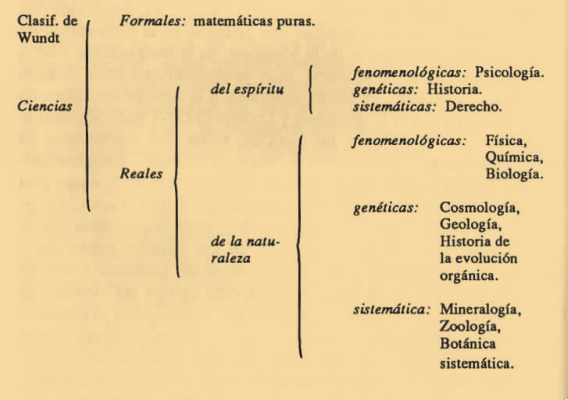
\includegraphics{wundt.png?raw=true}
\caption{Alt text}
\end{figure}

\hypertarget{el-derecho-y-la-sociedad}{%
\subsection{El Derecho y la Sociedad}\label{el-derecho-y-la-sociedad}}

La convivencia implica, inevitablemente, limitaciones a la esfera de la
libertad y del poder de cada cual, ajustes de los individuos entre sí y
de éstos con la sociedad, decía Máximo Pacheco en su libro Teoría del
Derecho. Santo Tomás de Aquino por otro lado señalaba que ``el objeto de
la justicia es el Derecho''. ghp\_8dkNarxV9FwLXxgBFBGWoGgmT2d08i35nUvQ
En términos generales podemos afirmar que el derecho consiste en aquella
regulación externa de la conducta de las personas, que busca establecer
un ordenamiento justo de la convivencia humana. Dado lo anterior, se
afirma que la existencia del Derecho en la sociedad es algo
consustancial, es decir, no puede existir sociedad sin derecho ni
derecho sin sociedad.

\hypertarget{clasificaciuxf3n-del-derecho}{%
\subsection{Clasificación del
Derecho}\label{clasificaciuxf3n-del-derecho}}

\begin{itemize}
\tightlist
\item
  \textbf{Derecho Natural}: es la expresión de los primeros principios
  de justicia que rigen las relaciones de los hombres en sociedad,
  determinan las facultades que a cada uno pertenecen de conformidad con
  el orden natural, y sirven de fundamento a toda regulación positiva de
  la convivencia humana.
\item
  \textbf{Derecho Positivo}: es el conjunto de normas de conducta
  bilaterales, imperativas y coactivas que regulan efectivamente la
  conducta de las personas en una sociedad con el objetivo de establecer
  un ordenamiento justo de la convivencia.
\end{itemize}

\hypertarget{fuentes-del-derecho}{%
\subsection{Fuentes del Derecho}\label{fuentes-del-derecho}}

Derecho, para estos efectos, debe ser entendido como \emph{derecho
objetivo y positivo}, en sentido de sistema de normas y decisiones
impuestas y tuteladas por el poder social. Por otro lado, la fuente del
derecho subjetivo es en último término el \textbf{derecho objetivo}, el
orden natural o positivo.

\begin{itemize}
\item
  \textbf{fuentes materiales} = son todos los factores que de forma
  directa o indirecta concurren en el nacimiento del derecho. Por fuente
  material \emph{directa} se entiende la sociedad por cuanto en ella se
  tiene origen la costumbre jurídica, los órganos legislativos, que dan
  nacimiento a la ley, y los tribunales de justicia, que generan
  sentencias. Por fuente material \emph{indirecta} se entiende todos
  aquellos elementos que de forma más o menos remota influye en el
  nacimiento o en la transformación del Derecho como los principios
  generales del derecho, las doctrinas religiosas, filosóficas y
  morales, los factores económicos-sociales, la labor de los juristas,
  las guerras, las revoluciones, el progreso técnico.
\item
  \textbf{fuentes formales} = son las formas en que el Derecho Positivo
  está contenido y se manifiesta en la vida social, se trata de la forma
  de expresión del derecho: la ley, la costumbre, las sentencias, la
  opinión de algunos tratadistas (doctrina) y los tratados
  internacionales.
\end{itemize}

\begin{figure}
\centering
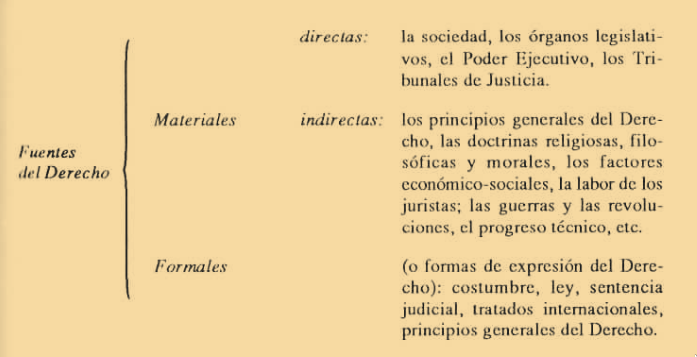
\includegraphics{fuentes.png?raw=true}
\caption{Alt text}
\end{figure}

\hypertarget{la-norma}{%
\subsection{La Norma}\label{la-norma}}

Las normas que tienen por finalidad regular la conducta de la persona
tienen por fin realizar valores. Pueden ser clasificadas de diversas
maneras, siendo la clasificación más común: - Normas de \textbf{trato
social}, las cuales tienen como fundamento la buena educación, decoro,
protocolo o cortesía. - Normas \textbf{morales}, las cuales regulan la
conducta libre de la persona que tienen por finalidad la trascendencia
del ser conforme a su cosmovisión. - Normas \textbf{jurídicas}, las
cuales pasaremos a estudiar en seguida.

\hypertarget{la-norma-juruxeddica}{%
\subsubsection{La norma jurídica}\label{la-norma-juruxeddica}}

Mandato dirigido a toda persona que viva en sociedad y mediante el cual,
bajo amenaza de sanción, se le conmina a observar una determinada
conducta positiva o negativa. Además, tiene por finalidad: a) asegurar
la \textbf{convivencia pacífica}; y b) \textbf{proteger sus intereses}
materiales y espirituales. Pacheco. ``Es una norma de conducta exterior,
bilateral, imperativa y coercitiva que regula la conducta de las
personas con el fin de establecer un ordenamiento justo de convivencia
humana''.

\hypertarget{quuxe9-diferencia-existe-entre-una-ley-y-una-norma}{%
\subsubsection{¿Qué diferencia existe entre una ley y una
norma?}\label{quuxe9-diferencia-existe-entre-una-ley-y-una-norma}}

Según Pacheco, el concepto de normas es más \textbf{amplio}, dado que la
norma puede expresarse también a través de la costumbre y de las
sentencias de los tribunales de justicia. En segundo lugar, la ley
requiere, necesariamente de un \textbf{legislador, promulgación y
vigencia}.

\hypertarget{clasificaciuxf3n-de-las-normas-juruxeddicas}{%
\subsubsection{Clasificación de las normas
jurídicas}\label{clasificaciuxf3n-de-las-normas-juruxeddicas}}

\begin{itemize}
\tightlist
\item
  Normas de Derecho Público y de Derecho Privado: Son de derecho público
  aquellas en que existe una relación de subordinación entre las partes,
  Estado y personas. En las de derecho privado existe una relación de
  igualdad entre las partes, que puede ser incluso el Estado una de
  ellas pero actuando como un privado.
\item
  Normas de Orden público y de Orden privado: Las normas de orden
  público existe un interés superior que se resguarda por lo que no
  pueden ser disponibles por las partes, es decir, no son derogables ni
  renunciables por ellas. Las normas de orden privado están puestas en
  beneficio de las personas y ellas pueden renunciar y disponer cuando
  así lo quieran. art. 12 CC
\end{itemize}

\hypertarget{caracteruxedsticas-de-las-normas-juruxeddicas}{%
\subsubsection{Características de las normas
jurídicas}\label{caracteruxedsticas-de-las-normas-juruxeddicas}}

\begin{itemize}
\tightlist
\item
  \emph{Exterioridad}: A la norma jurídica le preocupa la acción humana
  sólo desde el momento en que ella se ha \textbf{exteriorizado}.
\item
  \emph{Bilateralidad}: las normas jurídicas imponen deberes y
  correlativamente conceden facultades.
\item
  \emph{Determinación}: la norma jurídica generalmente se presenta con
  un contenido fijo cierto y reconocible. En su defecto, su sentido debe
  determinar su verdadero alcance.
\item
  \emph{Imperatividad}: Es de la esencia de toda norma jurídica el
  \textbf{ordenar} la realización o la abstención de una determinada
  conducta. Las primeras se denominan: normas jurídicas imperativas y
  las segundas, prohibitivas. 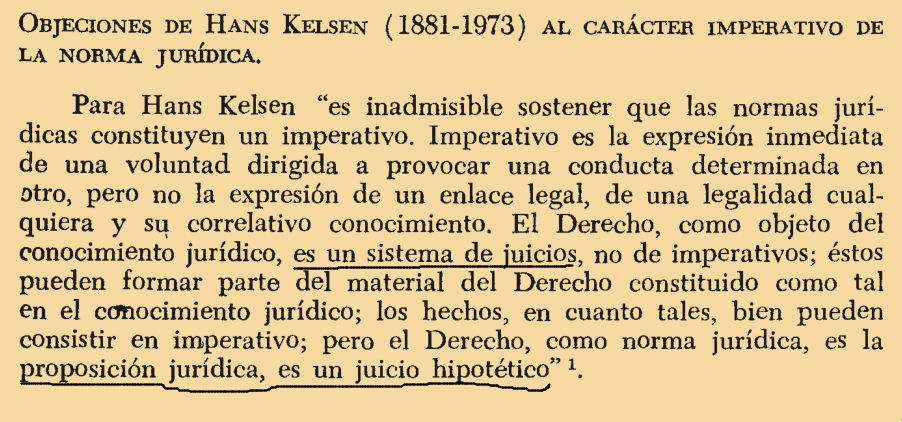
\includegraphics{objkelsen.png?raw=true}
\item
  \emph{Coactividad}: La norma jurídica constituye un imperativo que es
  susceptible de ser impuesto coactivamente.
\item
  \emph{Finalidad}: Que busca establecer un ordenamiento justo por el
  cual se pueda lograr el bien común.
\end{itemize}

\hypertarget{teoruxeda-de-la-ley}{%
\subsection{1.1. Teoría de la Ley}\label{teoruxeda-de-la-ley}}

\hypertarget{concepto}{%
\subsubsection{Concepto}\label{concepto}}

Planiol. ``Es una regla social obligatoria, establecida con carácter de
permanente por la autoridad pública, y sancionada por la fuerza''.

\begin{itemize}
\item
  Conceptos legales

  art. 1 CC La ley es una declaración de la voluntad soberana que
  manifestada en la forma prescrita por la CPR, manda prohíbe o permite.

  art. 63 Sólo son materias de ley: Nº 20, toda otra norma de carácter
  general y obligatoria que estatuya las bases esenciales de un
  ordenamiento jurídico.
\end{itemize}

\hypertarget{clasificaciuxf3n}{%
\subsubsection{Clasificación}\label{clasificaciuxf3n}}

\begin{enumerate}
\def\labelenumi{\arabic{enumi}.}
\item
  Normativas, Modificatorias, Interpretativas - prohibitivas

  Contiene un mandato de no hacer algo y no lo permite bajo ninguna
  circunstancia

  art. 10 los actos que prohíbe la ley son nulos y de ningún valor
  (absoluta), excepto que el legislador haya asignado otra sanción
\end{enumerate}

\begin{itemize}
\item
  imperativas

  Son las que imponen la obligación de hacer algo o el cumplimiento de
  un requisito.

  \begin{itemize}
  \tightlist
  \item
    sanción

    \begin{itemize}
    \item
      orden público

      Nulidad absoluta o relativa
    \item
      interés privado

      Sera generalmente la responsabilidad
    \end{itemize}
  \end{itemize}
\item
  permisivas

  Son aquellas que confieren un derecho que queda entregado al arbitrio
  del titular, y otorgan a el, los medios para obtener el reconocimiento
  de su derecho o la indemnización de los perjuicios que le acarrea su
  desconocimiento.
\end{itemize}

\hypertarget{efectos-en-el-tiempo}{%
\subsubsection{Efectos en el tiempo}\label{efectos-en-el-tiempo}}

art. 6 La ley no obliga sino una vez promulgada en conformidad a la CPR
y publicada conforme a las normas establecidas en los art. 7 y 8 CC.

art. 9 Sólo puede disponer para lo futuro y no tendrá jamás efecto
retroactivo

\begin{itemize}
\item
  La retroactividad en materia penal

  art. 19 Nª 3.8 CPR Ningún delito se castigará con otra pena que la que
  señale una ley promulgada con anterioridad a su perpetración, a menos
  que una nueva ley favorezca al afectado

  art. 18.2 CP Si la ley que exima el hecho de toda pena o le aplique
  una menos rigurosa se promulgare después de ejecutoriada la sentencia
  sea que se haya o no cumplido el TRB que hubiere pronunciado dicha
  sentencia, en 1ª o única deberá modificarla de oficio o a petición de
  parte
\item
  La retroactividad en materia civil

  Se encuentra principalmente limitada por el art. 19 Nª 24. Nadie
  pueden en caso alguno, \textbf{ser privado de su propiedad},
  \textbf{del bien sobre que recae} o de \textbf{alguno de los atributos
  o facultades} esenciales del dominio, sino en virtud de una
  \textbf{ley} general o especial que \textbf{autorice la expropiación}
  por causa de \textbf{utilidad pública o de interés nacional},
  calificada por el juez.
\item
  Ley de Efecto Retroactivo de las Leyes

  Tiene como objetivo decidir los conflictos que resultaren de la
  aplicación de leyes dictadas en diversas épocas y se inspira en la
  teoría de los derechos adquiridos y meras expectativas.

  \begin{itemize}
  \item
    Derechos adquiridos

    Derecho que por un hecho o acto del hombre o solo ministerio de la
    ley se ha incorporado al patrimonio, también se entiende por la
    facultad legalmente ejercida.
  \item
    Meras expectativas

    Derecho no incorporado al patrimonio o, facultad no ejercida
    legalmente
  \end{itemize}
\item
  Ultractividad de la ley

  art. 22 LERL ``en todo contrato se entenderán incorporadas las leyes
  vigentes al tiempo de su celebración''. Es decir, que pese a la
  modificación de las leyes, aquellas que se entendían incorporadas al
  contrato permanecerán vigentes.
\end{itemize}

\hypertarget{efectos-en-el-territorio}{%
\subsubsection{Efectos en el
territorio}\label{efectos-en-el-territorio}}

\begin{itemize}
\item
  Territorialidad

  art. 14 CC ``la ley es obligatoria para todos los habitantes de la
  república, incluso los extranjeros''.
\item
  Qué se entiende por territorio?

  \begin{itemize}
  \tightlist
  \item
    Es un concepto geográfico por el cual el Estado ejerce su
    jurisdicción, el cual se encuentra delimitado por sus fronteras, las
    posesiones chilenas en la Antártica (Territorio Chileno Antártico) y
    en Oceanía (Isla de Pascua)

    \begin{itemize}
    \item
      Territorio terrestre

      El cual comprende el suelo y subsuelo
    \item
      Espacio aéreo

      Consiste en la porción atmosférica terrestre
    \item
      Espacio marítimo

      Consiste en la prolongación del espacio terrestre haca el mar y
      comprende:

      \begin{enumerate}
      \def\labelenumi{\arabic{enumi}.}
      \tightlist
      \item
        el mar territorial, como extensión de soberanía que va desde la
        costa hasta las 12 millas marinas
      \item
        zona contigua, en que el Estado ejerce jurisdicción y se
        extiende hasta las 24 millas marinas
      \item
        mar patrimonial, que es una zona económica exclusiva de 200
        millas
      \end{enumerate}
    \item
      Espacio jurídico

      Consisten en lugares que por los tratados internacionales y la
      costumbre internacional reconocen como parte de la jurisdicción
      estatal.
    \end{itemize}
  \end{itemize}
\item
  Extraterritorialidad

  \begin{itemize}
  \item
    aplicación de la ley chile fuera del territorio de Chile

    Sólo produce efecto respecto de los chilenos sólo respecto a las
    siguientes materias:

    \begin{enumerate}
    \def\labelenumi{\arabic{enumi}.}
    \tightlist
    \item
      art. 15 ``a las leyes patrias que reglan las obligaciones y
      derechos civiles, permanecerán los chilenos, no obstante su
      residencia o domicilio en país extranjero''
    \item
      En lo relativo al estado de las personas y su capacidad para
      ejecutar ciertos actos, que hayan de tener efecto en Chile.
    \item
      En las obligaciones y derechos que nacen de las relaciones de
      familia, pero sólo respecto de sus cónyuges y parientes chilenos
    \end{enumerate}
  \item
    aplicación de ley extranjera en Chile
  \end{itemize}

  \begin{enumerate}
  \def\labelenumi{\arabic{enumi}.}
  \tightlist
  \item
    art. 16 CC da valor a las estipulaciones contenidas en los contratos
    otorgados válidamente en país extranjero (ley del contrato = se
    entienden incorporadas a él todas la leyes vigentes en ese momento,
    en territorio extranjero).

    \begin{itemize}
    \item
      Excepción o salvedad

      Sin perjuicio que sus efectos se arreglan a las leyes chilenas.
    \end{itemize}
  \item
    art. 955 inc. 2 establece que la sucesión se rige por la ley del
    domicilio en que se abre, por lo que la sucesión de una persona que
    muere en el extranjero se rige por las leyes de ese país.
  \end{enumerate}

  \begin{itemize}
  \tightlist
  \item
    Excepción o salvedad

    \begin{enumerate}
    \def\labelenumi{\arabic{enumi}.}
    \tightlist
    \item
      respecto a los bienes situados en Chile que forman parte del haber
      de la sucesión
    \item
      art. 998 tendrán los chilenos a título de herencia, la porción
      conyugal o de alimentos los mismos derechos que según las leyes
      chilenas les correspondería.
    \end{enumerate}
  \end{itemize}
\end{itemize}

\hypertarget{interpretaciuxf3n-de-la-ley}{%
\subsubsection{Interpretación de la
Ley}\label{interpretaciuxf3n-de-la-ley}}

Consiste en fijar su verdadero sentido y alcance, para lo cual se ha
establecido un conjunto de actividades indispensables para aplicar el
derecho a través de un sistema de interpretación reglada en los art. 19
a 24 CC Elementos de interpretación:

\begin{itemize}
\item
  Elemento gramatical

  Implica el análisis de la semántica y de la sintaxis del precepto.
  Señala el art. 19: "cuando el sentido de la ley es claro no se
  desatenderá su tenor literal, a pretexto de consultar su espíritu.
  Pero bien se puede, para interpretar una expresión obscura de la ley,
  recurrir a su intención o espíritu.

  El art. 20 "las palabras de la ley se entenderán en su sentido natural
  y obvio, según el uso general de las mismas palabras, pero cuando el
  legislador las haya definido expresamente para ciertas materias, se
  les dará en éstas su significado legal.
\item
  Elemento histórico

  Se refiere a la historia fidedigna del establecimiento de la ley
\item
  Elemento lógico

  Consiste en la \textbf{concordancia} que debe existir entre las
  diversas partes de la ley, que exista una unidad conceptual y de
  criterio
\item
  Elemento sistemático

  Debe existir una \textbf{correspondencia} más allá de la propia ley
  interpretada a otras leyes sobretodo si versan sobre la misma materia
\item
  Espíritu general del legislador y equidad natural

  La equidad es la justicia del caso concreto
\end{itemize}

\hypertarget{acto-juruxeddico}{%
\section{2. Acto Jurídico}\label{acto-juruxeddico}}

\hypertarget{hecho-juruxeddico}{%
\subsubsection{Hecho jurídico}\label{hecho-juruxeddico}}

Es todo suceso del hombre o de la naturaleza que produce efectos
jurídicos

\begin{itemize}
\tightlist
\item
  clasificación

  \begin{enumerate}
  \def\labelenumi{\arabic{enumi}.}
  \tightlist
  \item
    \textbf{con} intención de producir efectos jurídicos =
    \textbf{contratos}
  \item
    \textbf{sin} intención de producir efectos jurídicos
  \end{enumerate}

  \begin{itemize}
  \tightlist
  \item
    lícitos = \textbf{cuasicontratos}
  \item
    ilícitos = \textbf{delitos, cuasidelitos}
  \end{itemize}
\end{itemize}

\hypertarget{la-relaciuxf3n-juruxeddica}{%
\subsubsection{La relación jurídica}\label{la-relaciuxf3n-juruxeddica}}

Es aquella que existe entre dos o más personas, la cual está regulada
por el derecho objetivo. Este derecho objetivo le atribuye a uno de
ellos un poder y al otro un deber de encontrarse en la necesidad
jurídica de cumplir una determinada prestación para satisfacer el
interés que el sujeto titular del derecho está llamado a realizar con el
ejercicio de una acción que garantiza dicho derecho.

\hypertarget{acto-juruxeddico-1}{%
\subsubsection{Acto jurídico}\label{acto-juruxeddico-1}}

Es la manifestación o declaración de voluntad con la intención de
producir efectos jurídicos, los que pueden crear, modificar, transferir,
transmitir o extinguir derechos y obligaciones recíprocas. Hay autores
que agregan al final que dichos efectos son deseados por el autor o las
partes y sancionados por el derecho.

\begin{itemize}
\tightlist
\item
  requisitos

  \begin{itemize}
  \tightlist
  \item
    de \textbf{existencia}

    \begin{enumerate}
    \def\labelenumi{\arabic{enumi}.}
    \tightlist
    \item
      la voluntad
    \item
      el objeto
    \item
      la causa
    \item
      solemnidades cuando lo exige la ley
    \end{enumerate}
  \item
    de \textbf{validez}

    \begin{enumerate}
    \def\labelenumi{\arabic{enumi}.}
    \tightlist
    \item
      voluntad exenta de vicios
    \item
      objeto lícito
    \item
      causa lícita
    \item
      capacidad de las partes
    \end{enumerate}
  \end{itemize}
\item
  elementos

  \begin{itemize}
  \item
    de la esencia

    Son aquellos que sin los cuales el acto no produce efecto alguno o
    se degenera en otro diferente

    \begin{itemize}
    \item
      generales

      La doctrina tradicional entiende que son la voluntad, el objeto y
      la causa. J.A. Orrego señala por otro lado, que de la
      interpretación extensiva del art. 1444 se debe entender por ``no
      produce efecto alguno'', tantos los requisitos de existencia
      (excluyendo a la solemnidad) como los de validez.

      \begin{enumerate}
      \def\labelenumi{\arabic{enumi}.}
      \tightlist
      \item
        voluntad
      \item
        capacidad
      \item
        objeto
      \item
        causa
      \end{enumerate}
    \item
      especiales

      El que requiere cada acto o contrato para que produzca sus efectos
      propios y no se desvirtúe en otro, como el precio en la CV o la
      gratuidad en el comodato
    \end{itemize}
  \item
    de la naturaleza

    Son aquellos que se entienden incorporadas al acto sin necesidad de
    una cláusula especial
  \item
    accidentales

    son aquellos que sin ser de la esencia o de la naturaleza se pueden
    incorporar a los actos a través de cláusulas especiales, como ocurre
    en el caso de que las partes deseen establecer un plazo, condición o
    modo. Está fundado en el ppio. de autonomía de la voluntad
  \end{itemize}
\item
  Clasificación

  \begin{itemize}
  \item
    unilaterales o bilaterales

    Conforme al número de voluntades que requiere el acto, entendiendo
    que cada parte puede contar con una o varias personas. Son
    bilaterales los que requieren la manifestación de voluntad de dos o
    más partes que representen intereses contrapuestos o
    complementarios.
  \item
    entre vivos y por mortis causa

    Conforme a si requiere o no de la muerte de quien lo otorga, como
    sería el caso del testador.
  \item
    patrimoniales y de familia

    Conforme a si existe un interés preponderantemente pecuniario u otro
    de orden familiar con un interés general y común de fondo
  \item
    gratuitos y onerosos

    Conforme a si tiene por objeto la utilidad de una de las partes
    sufriendo la otra el gravamen, o si ambas partes se gravan a favor
    de la utilidad de ambas.

    \begin{itemize}
    \item
      onerosos conmutativos

      Son conmutativos aquellos en que el gravamen soportado se mira
      como equivalente a la utilidad percibida
    \item
      onerosos aleatorios

      Se denominan así aquellos actos bilaterales onerosos en que existe
      una contingencia incierta de ganancia o perdida
    \end{itemize}
  \item
    principales y accesorios

    Conforme a si subsisten por sí mismos o si requieren de otro para
    subsistir. Pueden ser de garantía asegurando el cumplimiento de una
    obligación principal, como en el caso de las cauciones tanto
    personales como reales. Como también pueden dependientes como en el
    caso de las capitulaciones matrimoniales
  \item
    solemnes y no solemnes

    Conforme a si requieren formalidades para su perfeccionamiento, los
    no formales son la r.g.
  \item
    puros y simples y sujetos a modalidad

    Conforme a si están sujetos a modalidad, la r. general es que sean
    puros y simples
  \item
    nominados e innominados

    Conforme a si se encuentran o no regulados por la ley
  \item
    actos de conservación, de administración y de disposición

    Administración = aquellos que tienden a la conservación y eventual
    incremento del patrimonio ajeno

    Disposición = aquellos que permiten al titular disminuir el
    patrimonio o el conjunto de bienes o una cosa determinada que una
    persona tiene a su cargo, mediante renuncia, abandono o enajenación
  \item
    actos simulados o verdaderos

    Conforme a la sinceridad de los contratantes

    Son simulados aquellos en los que la voluntad expresada o declarada
    no es coincidente con la verdadera voluntad del autor o de las
    partes

    Son verdaderos aquellos que reflejan la verdadera voluntad de las
    partes.
  \end{itemize}
\item
  Teorías y relación de ellas frente a las nuevas formas de contratación

  \begin{itemize}
  \item
    contratos celebrados mediante intermediarios

    Si son representantes, y actúan dentro de los límites de su
    representación, es cómo si los representados hubiesen celebrado el
    contrato directamente. Si no lo son, se tendrá por perfecto desde el
    momento en que los interesados aceptaren pura y simplemente la
    propuesta.
  \item
    contratos de adhesión

    Una de las partes, el oferente, fija de antemano todas las
    condiciones del contrato y la otra parte sólo puede adherir a ellas
    o rechazarlas en bloque. El adherente nada puede cambiar. Son
    dirigidos al público en general, la oferta se formula por un tiempo
    prolongado. El CC no los regula. Para impedir o morigerar la
    iniquidad se promulgó la ley del consumidor.
  \end{itemize}
\end{itemize}

\hypertarget{requisitos-del-acto-juruxeddico}{%
\subsubsection{Requisitos del Acto
Jurídico}\label{requisitos-del-acto-juruxeddico}}

\begin{itemize}
\item
  Son Requisitos de Existencia del Acto Jurídico:

  \begin{itemize}
  \tightlist
  \item
    Voluntad
  \item
    Objeto
  \item
    Causa
  \item
    Solemnidades en los casos que la ley lo exige
  \end{itemize}
\item
  Son Requisitos de Validez del Acto jurídico:

  \begin{itemize}
  \tightlist
  \item
    Voluntad exenta de vicios
  \item
    Objeto lícito
  \item
    Causa lícita
  \item
    Capacidad de las partes
  \end{itemize}
\item
  La Voluntad

  \begin{itemize}
  \item
    requisitos:

    \begin{itemize}
    \item
      \begin{enumerate}
      \def\labelenumi{\alph{enumi})}
      \tightlist
      \item
        exteriorizarse
      \end{enumerate}

      La voluntad debe manifestarse ya sea de manera expresa o tácita.
      El silencio no se considera expresión de voluntad. Se entiende que
      es en términos expresos aquella que se manifiesta en términos
      claros, directos. Se entiende que es tácita aquella que se deduce
      inequívocamente del comportamiento de la persona.

      \begin{itemize}
      \tightlist
      \item
        casos excepcionales en que el silencio se considera como
        manifestación de voluntad.

        \begin{enumerate}
        \def\labelenumi{\arabic{enumi}.}
        \tightlist
        \item
          Cuando las partes lo hayan acordado, como en el caso de la
          cláusula de renovación automática en la sociedad
        \item
          Cuando la ley le reconoce eficacia como en el caso del art.
          2125 (caso del mandado respecto a aquellas personas que por su
          profesión u oficio se encargan de negocios ajenos, de aceptar
          o no el encargo, su silencio se mirará como aceptación), o
          art. 1956 inc. 3 en el caso de la tácita reconducción.
        \item
          Silencio circunstanciado, el que va acompañado de otras
          circunstancias que permiten considerarlo como manifestación
        \end{enumerate}
      \end{itemize}
    \item
      \begin{enumerate}
      \def\labelenumi{\alph{enumi})}
      \setcounter{enumi}{1}
      \tightlist
      \item
        debe ser seria
      \end{enumerate}

      Es decir, con la intención de obligarse y formulada por persona
      capaz
    \end{itemize}
  \item
    consentimiento

    En los actos jurídicos bilaterales el análisis de la voluntad es
    doble. Es decir, se estudia el acuerdo de dos o más voluntades sobre
    un mismo acto jurídicos que se complementan. La voluntad aquí se
    denomina consentimiento. Se rigen por las normas establecidas en el
    C. de Com. art. 97 y ss. y solamente se aplica a los actos
    consensuales y no a los formales ni a los reales.

    \begin{itemize}
    \item
      formación del consentimiento

      \begin{itemize}
      \item
        \begin{enumerate}
        \def\labelenumi{\alph{enumi})}
        \tightlist
        \item
          oferta
        \end{enumerate}

        Acto jurídico unilateral en que una persona le \textbf{propone}
        la celebración de un acto o contrato a otra.

        \begin{enumerate}
        \def\labelenumi{\arabic{enumi}.}
        \tightlist
        \item
          Seria
        \item
          Completa
        \item
          Destinada a celebrar un acto j.
        \end{enumerate}
      \item
        \begin{enumerate}
        \def\labelenumi{\alph{enumi})}
        \setcounter{enumi}{1}
        \tightlist
        \item
          aceptación
        \end{enumerate}

        Acto j. unilateral por el cual la persona a quien va dirigida la
        oferta se adhiere o manifiesta su conformidad.

        \begin{enumerate}
        \def\labelenumi{\arabic{enumi}.}
        \tightlist
        \item
          pura y simple
        \item
          en tiempo oportuno (dentro del plazo)
        \item
          tempestiva (mientras se encuentra vigente la oferta)
        \end{enumerate}
      \end{itemize}
    \item
      momento en que se perfecciona

      \begin{itemize}
      \item
        aceptación

        Desde el momento en que el destinatario de la oferta da su
        aceptación. R.G. en Chile.
      \item
        expedición

        Desde el momento en que se envía la aceptación
      \item
        información

        desde que se ha recibido la aceptación y ha tomado conocimiento
        real y efectivo de ella
      \item
        recepción

        desde que ha llegado la aceptación a su destino
      \end{itemize}
    \item
      lugar en que se perfecciona

      en la residencia del que hubiere aceptado la propuesta
    \end{itemize}
  \end{itemize}
\item
  Los Vicios del Consentimiento

  \begin{itemize}
  \item
    \begin{enumerate}
    \def\labelenumi{\alph{enumi})}
    \item
      error

      consiste en la falta de conocimiento o la errónea representación
      de la realidad que puede recaer sobre una persona, un hecho o la
      ley

      \begin{itemize}
      \item
        esencial

        impide la formación del consentimiento y puede recaer sobre

        \begin{enumerate}
        \def\labelenumii{\arabic{enumii}.}
        \tightlist
        \item
          la naturaleza o especie del acto o contrato
        \item
          la identidad específica de la cosa de que se trata
        \end{enumerate}

        sanción = n.~absoluta, n.~relativa, inexistencia

        \begin{itemize}
        \item
          sustancial

          recae sobre la sustancia o calidad esencial del objeto.

          sanción = n.~relativa
        \item
          accidental

          no vicia el consentimiento, salvo que

          \begin{enumerate}
          \def\labelenumii{\arabic{enumii}.}
          \tightlist
          \item
            sea el motivo principal o determinante
          \item
            sea conocido por la otra parte
          \end{enumerate}

          sanción = n.~relativa
        \item
          persona

          no vicia el consentimiento, salvo que se trata de un contrato
          que se celebre en consideración a la persona, \emph{intuito
          personae}.

          sanción = n.~relativa e indemnización de perjuicios
        \item
          común

          se considera válido el acto a pesar de no estar ajustado a
          derecho

          \begin{enumerate}
          \def\labelenumii{\arabic{enumii}.}
          \tightlist
          \item
            debe ser compartido por todos o mayoría
          \item
            debe ser excusable, tener justo motivo
          \item
            buena fe
          \end{enumerate}
        \end{itemize}
      \end{itemize}
    \end{enumerate}

    \begin{itemize}
    \item
      \begin{enumerate}
      \def\labelenumi{\alph{enumi})}
      \setcounter{enumi}{1}
      \tightlist
      \item
        fuerza
      \end{enumerate}

      consiste en la coacción física o moral, actual o inminente,
      dirigida sobre la voluntad de una persona, con actos materiales o
      por medio de amenazas, para determinarla a consentir en un acto
      jurídico. Cuando es moral vicia el consentimiento, cuando es
      física no vicia el consentimiento, simplemente no hay voluntad.

      \begin{itemize}
      \tightlist
      \item
        requisitos:

        \begin{itemize}
        \item
          grave

          \begin{enumerate}
          \def\labelenumi{\arabic{enumi}.}
          \tightlist
          \item
            debe ser capaz de producir una impresión fuerte en una
            persona de sano juicio, tomando en cuenta su edad, sexo, y
            condición
          \item
            presunción en justo temor de verse ella, su consorte,
            ascendientes o descendientes a un mal irreparable o grave
          \item
            el temor reverencial no vicia el consentimiento
          \end{enumerate}
        \item
          ilegítima

          debe no estar autorizada por ley
        \item
          determinante

          sin ella no se hubiere prestado su consentimiento
        \item
          actual o inminente

          al momento de prestarse el consentimiento
        \end{itemize}
      \end{itemize}
    \item
      \begin{enumerate}
      \def\labelenumi{\alph{enumi})}
      \setcounter{enumi}{2}
      \tightlist
      \item
        dolo
      \end{enumerate}

      \begin{enumerate}
      \def\labelenumi{\arabic{enumi}.}
      \tightlist
      \item
        es la intención positiva de inferir injuria a la persona o
        propiedad de otro
      \item
        es un vicio del consentimiento constituido por la maquinación
        fraudulenta destinada a que una persona preste su consentimiento
        para la celebración de un acto o contrato.
      \end{enumerate}

      \begin{itemize}
      \tightlist
      \item
        clasificación

        \begin{enumerate}
        \def\labelenumi{\arabic{enumi}.}
        \tightlist
        \item
          dolo positivo y negativo
        \item
          dolo determinante e incidental
        \item
          dolo bueno y malo
        \end{enumerate}
      \item
        requisitos

        \begin{enumerate}
        \def\labelenumi{\arabic{enumi}.}
        \tightlist
        \item
          ser obra de una de las partes
        \item
          determinante
        \end{enumerate}
      \end{itemize}

      sanción = n.~relativa

      \begin{itemize}
      \tightlist
      \item
        características

        \begin{enumerate}
        \def\labelenumi{\arabic{enumi}.}
        \tightlist
        \item
          no se presume (salvo los casos de error de derecho en la
          posesión, indignidades para suceder, mera tenencia en la
          prescripción)
        \item
          no puede condonarse con anticipación
        \end{enumerate}
      \end{itemize}
    \end{itemize}
  \end{itemize}
\item
  la capacidad

  Se refiere a la capacidad de ejercicio, la aptitud de obligarse por sí
  mismo sin la autorización o ministerio de otra persona.

  \begin{itemize}
  \item
    clasificación

    se refiere a las clases de incapacidades de ejercicio que pueden
    existir

    \begin{itemize}
    \item
      incapacidad absoluta

      \begin{enumerate}
      \def\labelenumi{\arabic{enumi}.}
      \tightlist
      \item
        dementes
      \item
        impúberes
      \item
        sordos o sordomudos que no puedan darse a entender claramente
      \end{enumerate}

      \begin{itemize}
      \item
        cómo deben actuar?

        sólo actúan a través de sus representantes legales
      \item
        sanción

        \begin{enumerate}
        \def\labelenumi{\alph{enumi}.}
        \setcounter{enumi}{13}
        \tightlist
        \item
          absoluta
        \end{enumerate}
      \end{itemize}
    \item
      incapacidad relativa

      \begin{enumerate}
      \def\labelenumi{\arabic{enumi}.}
      \tightlist
      \item
        menores adultos
      \item
        los disipadores que se hallen bajo interdicción de administrar
        lo suyo
      \end{enumerate}

      \begin{itemize}
      \item
        cómo deben actuar? Deben cumplir con las llamadas ``formalidades
        habilitantes''.

        \begin{enumerate}
        \def\labelenumi{\arabic{enumi}.}
        \tightlist
        \item
          \textbf{autorizados} por su representante legal
        \item
          \textbf{a través} de sus representantes legales
        \end{enumerate}
      \item
        sanción

        \begin{enumerate}
        \def\labelenumi{\alph{enumi}.}
        \setcounter{enumi}{13}
        \tightlist
        \item
          relativa
        \end{enumerate}
      \end{itemize}
    \item
      incapacidades especiales o particulares

      es la prohibición que la ley ha impuesto a ciertas personas para
      ejecutar ciertos actos

      \begin{itemize}
      \tightlist
      \item
        casos
      \end{itemize}

      \begin{enumerate}
      \def\labelenumi{\arabic{enumi}.}
      \tightlist
      \item
        art. 412 respecto del curador y su pupilo. Sanción = n.~relativa
      \item
        art. 1796 CV entre cónyuges = n.~absoluta
      \item
        art. 1798 CV empleado público, bienes públicos que se vendan por
        su ministerio = n.~absoluta
      \item
        art. 114 menor adulto se casare sin consentimiento de su
        ascendiente = desheredamiento (testamentaria) y mitad de la
        porción que le hubiere correspondido (abintestato)
      \end{enumerate}
    \end{itemize}
  \end{itemize}
\item
  El objeto

  art. 1460 toda declaración de voluntad debe tener por objeto una o más
  cosas que se trata de dar, hacer o no hacer.

  \begin{itemize}
  \tightlist
  \item
    requisitos

    \begin{itemize}
    \tightlist
    \item
      sobre una cosa

      \begin{enumerate}
      \def\labelenumi{\arabic{enumi}.}
      \tightlist
      \item
        real
      \item
        comerciable
      \item
        determinada
      \item
        lícita
      \end{enumerate}
    \item
      sobre un hecho

      \begin{enumerate}
      \def\labelenumi{\arabic{enumi}.}
      \tightlist
      \item
        determinado
      \item
        físicamente posible
      \item
        moralmente posible
      \item
        lícito
      \end{enumerate}
    \end{itemize}
  \item
    casos de objeto ilícito en el CC

    \begin{enumerate}
    \def\labelenumi{\arabic{enumi}.}
    \tightlist
    \item
      actos y contratos contrarios al Dº público chileno
    \item
      pacto de sucesión de futura
    \item
      condonación del dolo futuro
    \item
      deudas contraídas en juegos de azar
    \item
      venta de libros cuya circulación es prohibida y otros objetos
      inmorales
    \item
      la enajenación en las cosas señaladas en el art. 1464
    \item
      art. 1466 generalmente en todo contrato prohibido por las leyes
    \end{enumerate}
  \end{itemize}
\item
  La causa

  El art. 1467.2 ``se entiende por causa el motivo que induce al acto o
  contrato y por causa ilícita la prohibida por ley, o contraria a las
  buenas costumbres o al orden público''

  \begin{itemize}
  \item
    Doctrina Causalista

    \begin{itemize}
    \item
      Doctrina Francesa o Clásica

      Postula que el acto jurídico debe tener una causa, junto con la
      voluntad y un objeto. Conciben la causa en términos objetivos y
      vinculada con la obligación
    \item
      Doctrina Italiana

      Considera la causa con un criterio subjetivo, aludiendo a los
      móviles que determinan a contratar, vinculan a la causa con el
      contrato.

      El análisis de la causa debe centrarse en la causa del acto o
      contrato, en el negocio, y no en la obligación que éste genera. La
      causa del acto o contrato, será de esta forma la función
      económica- social que caracteriza al tipo de negocio.
    \end{itemize}
  \item
    Doctrina Anticausalista

    Para estos la causa es un requisito artificial y prescindible. Es
    una noción falsa por cuanto:

    \begin{enumerate}
    \def\labelenumi{\arabic{enumi}.}
    \tightlist
    \item
      En los contratos bilaterales nacen simultáneamente por lo que no
      podría ser causa de la otra
    \item
      En los contratos reales no es causa de la obligación sino un
      requisito para que el contrato nazca
    \item
      En los gratuitos se confunde con los motivos
    \end{enumerate}

    Es inútil por cuanto:

    \begin{enumerate}
    \def\labelenumi{\arabic{enumi}.}
    \tightlist
    \item
      En los bilaterales la falta de causa implicaría la falta de objeto
      de la otra
    \item
      en los unilaterales y reales bastaría afirmar que no hay contrato
    \item
      En los gratuitos bastaría afirmar que no hay voluntad
    \end{enumerate}
  \item
    Réplica causalista Capitant

    No es falsa:

    \begin{enumerate}
    \def\labelenumi{\arabic{enumi}.}
    \tightlist
    \item
      En los bilaterales la causa de una obligación de una de las partes
      es la consideración de la obligación que la otra contraerá y
      viceversa.
    \item
      En los reales la misma prestación puede desempeñar ambos roles.
    \item
      en los gratuitos sirve para distinguir de los onerosos y para
      probar la utilidad.
    \end{enumerate}

    No es inútil:

    \begin{enumerate}
    \def\labelenumi{\arabic{enumi}.}
    \tightlist
    \item
      Bilaterales, la razón de la nulidad (por falta de objeto) está
      precisamente en la noción de causa y su interdependencia de ambas
      obligaciones por la causalidad
    \item
      De la causa de los contratos bilaterales se desprende la acción
      resolutoria, la teoría de los riesgos, la excepción de contrato no
      cumplido
    \item
      La capacidad, el consentimiento y el objeto están al servicio de
      la causa ya que este es el fin perseguido, luego sería el elemento
      principal y primario del acto.
    \end{enumerate}
  \item
    Acepciones de la palabra causa en la doctrina

    \begin{itemize}
    \item
      Causa eficiente

      Es el elemento generador del acto, es el antecedente y origen de
      algo, la causa de las obligaciones en este caso son el contrato,
      el cuasicontrato, el delito, el cuasidelito y la ley.
    \item
      Causa ocasional

      Los motivos individuales, personales de cada parte, diferentes de
      una a otra persona, permaneciendo generalmente en el fuero interno
      de cada individuo, sin expresarse. Es lo que se considera la causa
      del contrato.
    \item
      Causa final

      Es el fin o propósito inmediato e invariable de un acto, es la
      razón o interés jurídico que induce a obligarse, la finalidad
      típica y constante, cualquiera sea la persona que contrate y
      cualquiera que sean sus móviles particulares. Es lo que se
      considera como la causa de la obligación.
    \item
      Causa económica

      Se concibe como causa del contrato, la doctrina italiana expone
      sobre esto, los motivos por el cual las personas realizan un acto
      o contrato.
    \end{itemize}
  \item
    Características

    \begin{enumerate}
    \def\labelenumi{\arabic{enumi}.}
    \tightlist
    \item
      real
    \item
      no es necesario expresarla
    \item
      lícita
    \end{enumerate}
  \end{itemize}
\item
  Las formalidades

  son los requisitos externos con que deben ejecutarse o celebrarse
  algunos actos jurídicos, por disposición de la ley.

  \begin{itemize}
  \tightlist
  \item
    clasificación

    \begin{itemize}
    \item
      solemnidades

      Requisitos que establece la ley como indispensables para la
      existencia misma o para la validez del acto jurídico, exigidos en
      atención a la naturaleza o especie del acto o contrato

      sanción = inexistencia, n.~absoluta
    \item
      formalidades habilitantes

      son los requisitos externos exigidos por la ley en atención a la
      calidad o estado de las personas que ejecutan o celebran el acto o
      contrato.

      sanción = n.~relativa
    \item
      formalidades de prueba

      son los que sirven como el principal medio de prueba de un
      determinado acto o contrato.

      sanción = priva a las partes de un medio de prueba que les permita
      acreditar el contrato y sus obligaciones, y además, eventualmente,
      hacer fe de lo que declare una de las partes contratantes por
      sobre lo que declare la otra de las partes del contrato
    \item
      formalidades de publicidad

      son aquellos para poner en conocimiento de los terceros el
      otorgamiento o celebración de un acto o contrato

      simple noticia = poner en conocimiento de terceros de las
      relaciones j. que pueda tener interés = responsabilidad
      (indemnizar perjuicios)

      formalidades sustanciales = buscan precaver a los llamados
      terceros interesados, que son los que están o estarán en
      relaciones jurídicas con las partes = ineficacia del acto j.
      respecto a terceros (inoponibilidad)
    \item
      formalidades voluntarias

      las partes pueden hacer solemne un acto que por exigencia de la
      ley no tiene tal naturaleza = si no cumplen se entiende renunciada
    \end{itemize}
  \end{itemize}
\end{itemize}

\hypertarget{las-modalidades}{%
\subsection{2.5. Las Modalidades}\label{las-modalidades}}

\begin{itemize}
\item
  concepto

  consisten en elementos accidentales que se pueden introducir por las
  partes en virtud del principio de autonomía de la voluntad que tiene
  por propósito alterar los efectos propios del acto jurídico, ya sea
  con relación a su nacimiento, exigibilidad o extinción del mismo.
\end{itemize}

\hypertarget{la-condiciuxf3n}{%
\subsubsection{La Condición}\label{la-condiciuxf3n}}

consiste en un hecho futuro e incierto del cual depende el nacimiento o
extinción de un derecho

\begin{itemize}
\tightlist
\item
  clases

  \begin{enumerate}
  \def\labelenumi{\arabic{enumi}.}
  \tightlist
  \item
    positiva = un hecho que deba acontecer
  \item
    negativa = un hecho que no deba acontecer
  \item
    posible = puede o no ocurrir
  \item
    imposible = contrario a naturaleza, leyes, buenas costumbres, orden
    público o es ininteligible
  \item
    suspensiva = de la cual depende el nacimiento de un dº.
  \item
    resolutoria = de la cual depende la extinción de un dº.
  \item
    potestativa = depende de un hecho voluntario del acreedor o deudor
  \item
    causal = es aquella que depende de la voluntad de un tercero
  \item
    mixta = depende de la parte de voluntad del acreedor, voluntad del
    tercero o un acaso
  \end{enumerate}
\item
  clasificación

  \begin{enumerate}
  \def\labelenumi{\arabic{enumi}.}
  \tightlist
  \item
    Condición resolutoria ordinaria = siempre que la condición no
    consista en el incumplimiento de la obligación
  \item
    CRT = envuelta en todos los contratos bilaterales, de no cumplirse
    por una de las partes lo pactado.
  \item
    Pacto comisorio = CRT expresada
  \end{enumerate}
\end{itemize}

\hypertarget{el-plazo}{%
\subsubsection{El Plazo}\label{el-plazo}}

consiste en un hecho futuro y cierto del cual depende la exigibilidad o
extinción de un acto

\begin{itemize}
\tightlist
\item
  clasificación

  \begin{enumerate}
  \def\labelenumi{\arabic{enumi}.}
  \tightlist
  \item
    legal, judicial y convencional
  \item
    expreso o tácito
  \item
    suspensivo y extintivo
  \end{enumerate}
\item
  extinción del plazo

  \begin{itemize}
  \item
    Renuncia

    si mira el solo interés del deudor puede ser renunciado por él.

    su mira el interés de ambas partes, no puede ser renunciado por una
    de ellas sin el consentimiento de la otra
  \item
    Vencimiento

    llegada del día establecido
  \item
    Caducidad
  \end{itemize}
\end{itemize}

(concepto en materia de obligaciones pag. 146) ``Es una sanción legal
que consiste en la extinción de un derecho por no haberse ejercido o
cumplido una formalidad legal dentro del plazo fatal que la misma ley
establece'' Institución de la cual el acreedor puede ejercer su derecho,
aun encontrándose pendiente el plazo, en los casos que la ley lo
establece o que se hubiere convenido expresamente. Clases de caducidad:

\begin{itemize}
\item
  caducidad legal = deudor en procedimiento concursal o notoria
  insolvencia, deudor cuyas cauciones han disminuido por hecho o culpa
  suya.
\item
  convencional = casos establecidos expresamente por las partes.
\end{itemize}

\hypertarget{el-modo}{%
\subsubsection{El Modo}\label{el-modo}}

Es el gravamen que se impone al beneficiario de una liberalidad. No
suspende la adquisición de la asignación, sin embargo, si está
establecida en beneficio de un tercero, éste puede exigir su
cumplimiento forzado. Entre vivos también se puede establecer siguiendo
las reglas del pacto comisorio (si se establece en contrato que no sea
CV o permuta) o de la CRT en caso de contrato bilateral

\hypertarget{ineficacia-de-los-actos-juruxeddicos}{%
\subsection{2.6. Ineficacia de los Actos
Jurídicos}\label{ineficacia-de-los-actos-juruxeddicos}}

\begin{itemize}
\item
  Qué es la eficacia de los actos jurídicos?

  Es la capacidad que debe tener el acto jurídico para lograr el efecto
  que se desea o espera.
\item
  Ineficacia en sentido amplio

  Se entiende por tal, cuando: a) un acto no genera sus efectos propios
  desde el momento mismo en que se otorgó o celebró; b) cuando habiendo
  generado sus efectos, deja de producirlos por cualquier causa. Dado lo
  anterior, podemos afirmar que esta definición incluye tanto la
  nulidad, como la inexistencia (ineficacia originaria)

  \begin{itemize}
  \item
    inexistencia

    consiste en una sanción civil establecida para la omisión de los
    requisitos de \textbf{existencia} de un acto, es decir, voluntad o
    consentimiento, objeto, la causa, o solemnidades.
  \item
    nulidad
  \end{itemize}
\end{itemize}

\begin{figure}
\centering
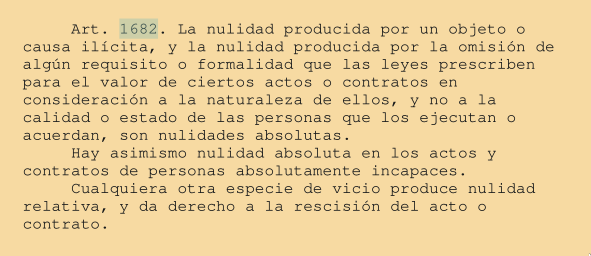
\includegraphics{1681.png?raw=true}
\caption{Alt text}
\end{figure}

\begin{itemize}
\item
  efectos:

  \begin{enumerate}
  \def\labelenumi{\arabic{enumi}.}
  \item
    sólo se producen una vez declarada por sentencia judicial
    ejecutoriada
  \item
    volver a las partes al estado que tenían antes de la celebración del
    acto nulo
  \item
    realizar las restituciones recíprocas
  \end{enumerate}

  \begin{itemize}
  \item
    respecto a terceros

    declarada judicialmente da acción reivindicatoria frente a terceros
    Excepciones: - (A) No da acción reivindicatoria respecto: 1.
    rescisión por lesión enorme 2. muerte presunta 3. donación entre
    vivos 4. tercero poseedor que adquiere por prescripción 5. acción de
    indignidad para suceder
  \end{itemize}
\item
  clases:

  \begin{itemize}
  \item
    Nulidad Absoluta

    Es la sanción legal impuesta a la omisión de los requisitos exigidos
    en consideración a la naturaleza o especie del acto.

    Procede en los ss. casos:

    \begin{enumerate}
    \def\labelenumi{\alph{enumi})}
    \item
      Falta requisito de existencia
    \item
      Objeto o causa ilícita
    \item
      Actos de los absolutamente incapaces
    \item
      Error esencial
    \end{enumerate}

    \begin{itemize}
    \item
      titulares

      \begin{enumerate}
      \def\labelenumi{\arabic{enumi}.}
      \item
        juez, aparezca de manifiesto
      \item
        todo aquél que tenga interés pecuniario en ello
      \item
        por el ministerio público en interés de la moral y la ley
      \end{enumerate}
    \end{itemize}
  \item
    Características

    \begin{enumerate}
    \def\labelenumi{\arabic{enumi}.}
    \tightlist
    \item
      puede y debe ser declarada de oficio por el juez
    \item
      puede alegarla todo el que tenga interés
    \item
      puede solicitarla el ministerio público
    \item
      no puede ratificarse\\
    \item
      es irrenunciable / Es de orden público
    \item
      no se produce de pleno derecho (al igual que la relativa)
    \end{enumerate}
  \item
    Nulidad Relativa

    Es la sanción por la omisión de algún requisito o formalidad que la
    ley exige en atención al estado o calidad de las partes. Está
    establecida para proteger los intereses de ciertas y determinadas
    personas, por lo que, no protege intereses generales. Procede:
  \end{itemize}

  \begin{enumerate}
  \def\labelenumi{\alph{enumi})}
  \tightlist
  \item
    respecto de los acto de los relativamente incapaces cuando se omiten
    las formalidades habilitantes.
  \item
    respecto del dolo principal y determinante
  \item
    Error substancial
  \item
    Fuerza moral
  \item
    Error accidental
  \item
    Error en la persona
  \item
    Omisión de un requisito establecido para la validez del acto
  \item
    En los casos en que se establece como sanción respecto a la lesión
  \end{enumerate}

  \begin{itemize}
  \tightlist
  \item
    Titulares

    \begin{enumerate}
    \def\labelenumi{\arabic{enumi}.}
    \tightlist
    \item
      personas en cuyo beneficio se ha establecido la norma
    \item
      herederos
    \item
      cesionarios
    \end{enumerate}
  \item
    Características

    \begin{itemize}
    \tightlist
    \item
      puede sanearse

      \begin{itemize}
      \tightlist
      \item
        por el trascurso del plazo para pedir rescisión = 4 años
      \item
        por la voluntad de las partes = ratificación o confirmación
        (salvo declaración judicial)
      \end{itemize}
    \item
      da lugar la acción reivindicatoria
    \item
      procedimiento: juicio ordinario
    \end{itemize}
  \end{itemize}
\item
  Defina ineficacia en el sentido estricto

  La causa de ineficacia se origina después de haberse otorgado o
  celebrado el acto. Es decir, el acto jurídico por sí idóneo, no genera
  sus efectos o deja de producirlos, por un hecho \textbf{extrínseco},
  una circunstancia usualmente sobreviniente o coetáneas y extrañas a su
  estructura.

  \begin{itemize}
  \tightlist
  \item
    Señale los casos de ineficacia en sentido estricto:

    \begin{itemize}
    \item
      La suspensión

      Los efectos de un acto están subordinados a la ocurrencia de un
      hecho. Puede ser producto de la voluntad de las partes, como en el
      caso de la condición suspensiva o del plazo suspensivo o, puede
      ser producto de la ley en el caso de una condición legal como es
      el caso de las disposiciones testamentarias.
    \item
      La resolución

      Los efectos de un acto pueden cesar y eliminarse la eficacia de
      los ya producidos, si sobreviene un hecho determinado, es un
      ejemplo la CRT.
    \item
      La revocación

      Consiste en una declaración unilateral de voluntad por la
      retractación de un acto, incluso bilateral cuando la ley así lo
      autoriza. Es ejemplo del primero el caso del testamento. Es
      ejemplo del segundo el caso del mandato.
    \item
      El desistimiento unilateral

      Una de las partes decide y comunica a la otra el término de una
      relación contractual, solamente cuando la ley lo autoriza, como
      por ejemplo el caso del desahucio en el contrato de arrendamiento.
    \item
      La caducidad

      Puede entenderse como la pérdida de un derecho por no hacerlo
      valer en el plazo legal o contractual. Como ineficacia opera por
      el solo ministerio de la ley en algunos casos como por ejemplo: en
      el testamento privilegiado, en las donaciones revocables (por
      mortis causa) las cuales caducan por la muerte del donatario antes
      del donante
    \item
      La resciliación

      Convención en virtud de la cual las partes de común acuerdo
      estipulan dejar sin efecto un contrato válidamente celebrado en la
      medida que sus efectos no estén totalmente cumplidos
    \item
      La inoponibilidad

      Consiste en la ineficacia de un acto jurídico o la ineficacia de
      su nulidad, respecto de ciertos terceros, por no haber cumplido
      las partes algún requisito externo o por lesionar intereses
      ajenos.
    \end{itemize}
  \end{itemize}
\end{itemize}

\hypertarget{teoruxeda-de-la-prueba-civil}{%
\subsection{2.7. Teoría de la Prueba
Civil}\label{teoruxeda-de-la-prueba-civil}}

\begin{itemize}
\item
  Qué se puede entender por prueba?

  \begin{enumerate}
  \def\labelenumi{\arabic{enumi}.}
  \tightlist
  \item
    Como \textbf{demostración} de la verdad de un hecho, de su
    existencia o inexistencia
  \item
    Como \textbf{medio de prueba}, medios de convicción.
  \item
    Como el hecho mismo de su producción, de hacerla valer ante TRB.
  \end{enumerate}
\item
  Por qué se dice que la prueba también es materia propia del Derecho
  Civil?

  El CPC contiene normas de la manera como se rinden las pruebas en un
  juicio o un acto judicial no contencioso, pero la materia sobre la
  prueba es también sustancial:

  \begin{enumerate}
  \def\labelenumi{\arabic{enumi}.}
  \tightlist
  \item
    porque existen situaciones que deben probarse fuera de juicio, como
    sería la edad mínima para celebrar el contrato de matrimonio.
  \item
    porque presenta una parte sustantiva, a) determina los medios de
    prueba, b) señala su admisibilidad, c) determina el valor probatorio
  \end{enumerate}
\item
  Cual es el objeto de la prueba?

  Son los \emph{hechos}, el derecho conforme al art. 8 CC no necesita
  probarse.

  \begin{itemize}
  \tightlist
  \item
    Señale las excepciones

    \begin{enumerate}
    \def\labelenumi{\arabic{enumi}.}
    \tightlist
    \item
      Cuando la norma de derecho emana de la costumbre. (es excepción
      porque se debe probar derecho)
    \item
      Los hechos pacíficos (no controvertidos) no requieren prueba. (es
      excepción porque no se debe probar un hecho)
    \item
      Los hechos notorios no requieren prueba (es excepción por lo mismo
      de lo anterior)
    \end{enumerate}
  \end{itemize}
\item
  Qué es el onus probandi?

  Es una carga, una subordinación de los intereses del titular de ellos
  a otro interés de el mismo. Es decir, no está obligado a probar, pero
  si no se prueba, sus pretensiones no serán acogidas por el juez.

  \begin{itemize}
  \item
    A quién incumbe probar?

    art. 1698 ``incumbe probar las obligaciones o su extinción al que
    alega aquellas o ésta''. Es decir, como principio general
    corresponde probar al que ha sostenido una proposición contraria al
    estado normal u ordinario de las cosas, o al que pretende destruir
    una situación adquirida.
  \end{itemize}
\item
  Clasifique los hechos jurídicos para efectos probatorios

  Estas normas se aplican también respecto de los elementos del acto
  jurídico.

  \begin{itemize}
  \item
    Hechos constitutivos

    Son aquellos que producen el nacimiento de un derecho o de una
    situación jurídica antes inexistente. Los genéricos (la capacidad,
    objeto, causa) no deben probarse. Los específicos si deben probarse.
    Por ejemplo en una CV se deberá probar que se acordó dar tal cosa y
    la otra pagar tal precio
  \item
    Hechos impeditivos

    Aquellos que impiden la generación válida de una relación jurídica.
    Deben probarse, como por ejemplo los vicios del consentimiento
  \item
    Hechos modificativos

    Son aquellos que alteran en su contenido o efectos la relación
    jurídica, deben probarse. Como por ejemplo las modalidades
  \item
    Hechos extintivos

    Son aquellos que hacen desaparecer una relación jurídica o sus
    efectos, deben probarse. Como lo son los modos de extinguir las
    obligaciones.
  \end{itemize}
\item
  Quién puede cambiar el peso de la prueba?

  La ley, estableciendo presunciones legales y la voluntad de las
  personas, a través de las convenciones entre las partes. Es decir, las
  normas del onus probandi son de orden privado y renunciables por las
  partes.
\item
  Cómo opera la prueba de los hechos negativos?

  Pueden y deben probarse, dado que toda proposición negativa implica
  una proposición positiva o afirmativa que es su antítesis. Si se
  sostiene que no estaba en X lugar, puede probar que estaba en el lugar
  Y.
\end{itemize}

\hypertarget{sujetos-de-derecho}{%
\section{3. Sujetos de Derecho}\label{sujetos-de-derecho}}

\begin{itemize}
\tightlist
\item
  Como se clasifican las personas?

  \begin{itemize}
  \item
    Personas naturales

    art. 55 Son personas todos los individuos de la especie humana,
    cualquiera sea su edad, sexo, estirpe o condición

    \begin{itemize}
    \item
      Requisitos para que el nacimiento constituya principio de
      existencia legal de la persona:

      \begin{enumerate}
      \def\labelenumi{\arabic{enumi}.}
      \tightlist
      \item
        Que sea separado completamente de la madre
      \item
        Debe haber sobrevivido a la separación un momento siquiera
      \end{enumerate}
    \item
      Qué es y hasta cuando dura la existencia natural de la persona?

      Se dice existencia natural la que principia en la concepción y
      termina en el nacimiento. el CC señala en el art. 75 ``la ley
      protege la vida del que está por nacer''
    \item
      Presunción de concepción

      art. 76 se presume de derecho que la época de concepción ha
      precedido al nacimiento en no menos de 180 días y no más de 300,
      contados hacia atrás, \textbf{desde la medianoche en que principie
      el día del nacimiento}.
    \item
      Qué efectos produce el nacimiento de una persona?

      \begin{enumerate}
      \def\labelenumi{\arabic{enumi}.}
      \tightlist
      \item
        Se termina la existencia natural y se \textbf{da comienzo a la
        existencia legal}
      \item
        Nacen los \textbf{atributos de la personalidad}
      \item
        art. 77 los derechos patrimoniales que se encontraban en
        suspenso \emph{se radican en el patrimonio} del recién nacido.
        Por lo que, si fallece, los transmitirá a sus herederos.
      \end{enumerate}
    \item
      Hasta cuándo dura la existencia legal de la persona?

      art. 78 La persona (se refiere a la existencia legla) termina en
      la muerte natural. Consiste en la cesación de los fenómenos de la
      vida, de las funciones respiratorias y encefálicas.
    \item
      Como se clasifica la muerte?

      \begin{itemize}
      \item
        Muerte real

        Es aquella que efectivamente consta que la persona murió y se
        certifica el cese de sus funciones vitales por un medico.

        \begin{itemize}
        \tightlist
        \item
          Qué efectos produce la muerte real de la persona?

          \begin{enumerate}
          \def\labelenumi{\arabic{enumi}.}
          \tightlist
          \item
            Da origen al modo de adquisición del dominio que es la
            sucesión por causa de muerte
          \item
            Pone fin a la personalidad del individuo (existencia legal)
          \item
            Pone fin al matrimonio
          \item
            Pone fin a la patria potestad
          \item
            Da fuerza legal al testamento
          \item
            Pone fin a ciertos contratos (intuito personae, o que tengan
            una preponderancia especial la consideración de la persona
            con la cual se contrata)
          \item
            Algunas instituciones terminan por la muerte de quien la
            desempeña (las guardas)
          \item
            Se extinguen determinadas acciones civiles como la acción de
            nulidad del matrimonio, salvo excepciones.
          \item
            Se extinguen los derechos intransmisibles como lo son el
            derecho a pedir alimentos, el usufructo, el uso o
            habitación.
          \end{enumerate}
        \end{itemize}
      \item
        Muerte presunta

        art. 81 se presume muerto al individuo que ha desaparecido,
        ignorándose si vive y verificándose las condiciónes que se
        señalan.

        \begin{itemize}
        \item
          Cuales son los elementos tomados en cuenta para presumir que
          la persona ha muerto?

          \begin{enumerate}
          \def\labelenumi{\arabic{enumi}.}
          \tightlist
          \item
            la ausencia o desaparecimiento
          \item
            la carencia de noticias sobre éste
          \end{enumerate}
        \item
          Qué toma en consideración la ley para que exista esta
          institución?

          \begin{enumerate}
          \def\labelenumi{\arabic{enumi}.}
          \tightlist
          \item
            Toma en consideración el interés de la persona desaparecida
          \item
            El interés de los terceros, respecto a eventuales derechos
            de sucesión
          \item
            El interés general de la sociedad en que no existan bienes o
            derechos abandonados
          \end{enumerate}
        \item
          Cuales son los requisitos para que proceda la declaración de
          muerte presunta?

          \begin{enumerate}
          \def\labelenumi{\arabic{enumi}.}
          \tightlist
          \item
            Que sea declarada por sentencia judicial
          \item
            Que se haga conforme a las disposiciones procesales del CPC
          \item
            Que el indivíduo haya desaparecido
          \item
            Que no se tenga noticia de su existencia
          \end{enumerate}
        \item
          Periodos o etapas de la muerte presunta

          \begin{enumerate}
          \def\labelenumi{\arabic{enumi}.}
          \tightlist
          \item
            mera ausencia
          \item
            posesión provisoria
          \item
            posesión definitiva
          \end{enumerate}
        \item
          Quiénes pueden pedir la declaración de muerte presunta?

          Cualquiera que tenga interés (\emph{pecuniario}) en su
          declaración. Los acreedores pueden dirigirse al apoderado del
          ausente o provocar el nombramiento de un curador.
        \item
          Quién es competente para declarar la muerte presunta de una
          persona?

          art. 81 CC y 151 COT el juez del último domicilio que el
          desaparecido haya tenido en Chile.
        \item
          Formalidades para la solicitud de declaración de muerte
          presunta

          \begin{enumerate}
          \def\labelenumi{\arabic{enumi}.}
          \tightlist
          \item
            los interesados deben justificar que \textbf{se ignora} el
            paradero del desaparecido y que se han hecho las posibles
            diligencias para encontrarlo
          \item
            \textbf{citación} del desaparecido, por 3 veces con
            diferencia de 2 meses entre cada una en el periódico oficial
          \item
            intervención del \textbf{defensor de ausente} (defensor
            público)
          \item
            todas las sentencias (interlocutorias y definitivas) deben
            ser \textbf{insertadas en periódico oficial}
          \item
            fijación del \textbf{día presuntivo} de la muerte (r. g. el
            último día del primer bienio)
          \end{enumerate}
        \item
          Qué es el periodo de mera ausencia?

          Es el que dura desde la fecha de las últimas noticias respecto
          del desaparecido hasta el decreto de posesión provisoria o
          definitiva, o por la reaparición del desaparecido o con la
          confirmación de su muerte.

          \begin{itemize}
          \tightlist
          \item
            Qué ocurre con la administración de los bienes?

            \begin{enumerate}
            \def\labelenumi{\arabic{enumi}.}
            \tightlist
            \item
              Si el desaparecido tiene representante legal le
              corresponderá a el
            \item
              Si dejo mandatario, le corresponderá a el
            \item
              Si no dejó mandatario y no tiene representante legal, se
              nombrará curador de ausentes (su nombramiento puede ser
              provocado por cualquiera que tenga interés patrimonial en
              ello)
            \end{enumerate}
          \end{itemize}
        \end{itemize}
      \end{itemize}
    \item
      Término del periodo de mera ausencia:

      \begin{itemize}
      \tightlist
      \item
        Decreto de posesión provisoria
      \item
        Decreto de posesión definitiva
      \item
        Reaparecimiento del ausente
      \item
        Conocimiento positivo de la fecha de muerte real del
        desaparecido.
      \end{itemize}
    \end{itemize}
  \item
    Qué es la posesión provisoria?

    Es aquella que empieza con la resolución que la declara y termina
    con la resolución judicial que concede la posesión definitiva.

    \begin{itemize}
    \item
      la cual, produce los siguientes \emph{efectos}

      \begin{enumerate}
      \def\labelenumi{\arabic{enumi}.}
      \item
        disuelve la sociedad conyugal
      \item
        se procederá a la apertura y publicación del testamento
      \item
        emancipación legal de los hijos, salvo que correspondiera al
        otro cónyuge
      \item
        la posesión provisoria sobre los bienes del desaparecido a los
        herederos presuntivos
      \end{enumerate}
    \end{itemize}
  \item
    Qué es la posesión definitiva?

    Es la resolución judicial que se declara cuando termina la posesión
    provisoria, produciendo los siguientes efectos:

    \begin{enumerate}
    \def\labelenumi{\arabic{enumi}.}
    \item
      pone fin a la posesión provisoria
    \item
      disuelve el matrimonio
    \item
      terminan las cauciones otorgadas para disponer de los bienes que
      se poseían provisoriamente
    \item
      se terminan las limitaciones para disponer de los bienes del
      desaparecido que tenían los herederos presuntivos
    \item
      se pueden hacer valer los derechos sujetos a la muerte del
      desaparecido, como en el caso del usufructo
    \item
      los legatarios pueden exigir sus derechos.

      \begin{itemize}
      \tightlist
      \item
        Cuando se decreta la posesión definitiva?

        \begin{enumerate}
        \def\labelenumii{\arabic{enumii}.}
        \tightlist
        \item
          cuando cumplido los 5 años (de la última noticia), se probare
          que el desaparecido tiene más de 70 años.
        \item
          Inmediatamente con el transcurso de los 5 años desde la fecha
          de la herida grave en la guerra o peligro similar
        \item
          Inmediatamente transcurrido 3 meses desde la fecha de la
          última noticia que se tuvieron de la nave o aeronave reputada
          perdida
        \item
          Inmediatamente luego de 6 meses desde sismo o catástrofe
        \item
          en último caso, transcurrido 10 años desde la última noticia
        \end{enumerate}
      \item
        Qué obligaciones protegen los bienes del desaparecido?

        \begin{enumerate}
        \def\labelenumii{\arabic{enumii}.}
        \tightlist
        \item
          inventario solemne
        \item
          caución de conservación y restitución
        \end{enumerate}
      \item
        Cuando autoriza la ley a pedir rescisión del decreto judicial de
        muerte presunta?

        \begin{enumerate}
        \def\labelenumii{\arabic{enumii}.}
        \tightlist
        \item
          si se tuvieren noticias de la existencia del desaparecido
        \item
          si hubiere noticias de la muerte real del desaparecido
        \item
          si reaparece.
        \end{enumerate}
      \item
        a favor de quiénes se puede rescindir?

        \begin{enumerate}
        \def\labelenumii{\arabic{enumii}.}
        \tightlist
        \item
          del desaparecido que reaparece
        \item
          los legitimarios habidos durante el desaparecimiento
        \item
          cónyuge
        \end{enumerate}
      \end{itemize}
    \end{enumerate}
  \end{itemize}
\item
  Son atributos de la personalidad:

  \begin{itemize}
  \item
    \begin{enumerate}
    \def\labelenumi{\alph{enumi})}
    \item
      \textbf{la nacionalidad}

      Consiste en el vínculo de derechos y obligaciones que une a
      individuo con el Estado por el hecho de haber adquirido la
      nacionalidad por alguna de las causales que establece la CPR
    \end{enumerate}

    art. 56 señala que son chilenos los que la CPR declara como tales,
    la CPR art. 10 señala que son chilenos:

    \begin{enumerate}
    \def\labelenumi{\arabic{enumi}.}
    \tightlist
    \item
      Los nacidos en territorio de Chile
    \item
      Los hijos de padre o madre chilenos, nacidos en territorio
      extranjero
    \item
      Los extranjeros que obtuvieren carta de nacionalización en
      conformidad a la ley
    \item
      Los que obtuvieren especial gracia de nacionalización por ley -
      Como se pierde la nacionalidad (art. 11 CPR)? 1. Por
      \textbf{renuncia voluntaria} si la persona se ha nacionalizado en
      país extranjero 2. Por \textbf{Decreto Supremo} en caso de
      prestación de servicios durante una guerra exterior a enemigos de
      Chile 3. Por \textbf{ley} que revoque la nacionalización concedida
      por gracia
    \end{enumerate}
  \item
    \begin{enumerate}
    \def\labelenumi{\alph{enumi})}
    \setcounter{enumi}{1}
    \item
      \textbf{el nombre}

      Conjunto de palabras que sirven para distinguir legalmente a una
      persona de otra.

      Ley 4.808 art. 30 La inscripción del nombre puede ser requerida
      por padre o madre por sí o por mandatario dentro de los 30 días
      siguientes al nacimiento de la criatura.

      art. 28, 29 se deberá hacer por las personas indicadas (padre,
      pariente más cercano mayor, medico que hubiera ocurrido al
      nacimiento, jefe del establecimiento) dentro de los 60 días.

      Se puede colocar cualquier nombre, salvo que sea extravagante,
      ridículo, impropio de persona, equívoco respecto a su sexo o
      contrario al buen lenguaje
    \end{enumerate}
  \item
    \begin{enumerate}
    \def\labelenumi{\alph{enumi})}
    \setcounter{enumi}{2}
    \item
      \textbf{el estado civil}

      Consiste en la calidad que tiene una persona en cuanto lo habilita
      para ejercer ciertos derechos y contraer ciertas obligaciones
      civiles

      \begin{itemize}
      \tightlist
      \item
        características

        \begin{enumerate}
        \def\labelenumii{\arabic{enumii}.}
        \tightlist
        \item
          es un atributo de la personalidad
        \item
          su regulación es de orden público
        \item
          es un derecho extra patrimonial (no se traspasa)
        \item
          es permanente, mientras no se adquiere otro
        \item
          es uno e indivisible, sin perjuicio de que se puede tener más
          de uno con relación a fuentes distintas, como pueden concurrir
          el de hijo, soltero y padre
        \item
          es imprescriptible
        \item
          es irrenunciable

          \begin{itemize}
          \item
            Cuales son los principales \emph{efectos} del estado civil?

            \begin{enumerate}
            \def\labelenumiii{\arabic{enumiii}.}
            \tightlist
            \item
              da origen a derechos y obligaciones
            \item
              da origen al parentesco

              \begin{itemize}
              \tightlist
              \item
                Clasificación

                \begin{itemize}
                \item
                  Natural o de consanguinidad

                  Es la relación de sangre entre dos personas que
                  descienden unas de las otras o de un tronco común
                \item
                  Legal o por afinidad

                  Es el que existe entre una persona que está o ha
                  estado casada y los consanguíneos de su marido o mujer
                \item
                  Adopción

                  Conforme a la Ley 19.620
                \end{itemize}
              \item
                Como se estructura el parentesco?

                \begin{itemize}
                \item
                  línea de parentesco

                  Consiste en el número de generaciones que existe entre
                  dos personas
                \item
                  línea colateral

                  Es aquella que se forma con el vínculo a un tronco
                  común
                \item
                  el grado

                  Es el número de generaciones que separan a los
                  parientes
                \end{itemize}
              \end{itemize}
            \end{enumerate}
          \item
            como se prueba el estado civil?

            A través de los certificados o partidas que emite el
            Registro Civil, los cuales constituyen instrumentos
            públicos.

            A falta de dichos instrumentos públicos, se puede probar
            por:

            \begin{enumerate}
            \def\labelenumiii{\arabic{enumiii}.}
            \tightlist
            \item
              Otros documentos auténticos (como seria un testamento en
              que se reconoce un hijo)
            \item
              Declaraciones de testigos presenciales al hecho (como lo
              sería la declaración del medico que constata la muerte de
              una persona)
            \item
              Por la posesión notoria del estado civil, en el caso del
              matrimonio, siempre que sea de nombre, trato y fama, a lo
              menos por 10 años de forma pública y continua.
            \end{enumerate}
          \item
            cuales son las fuentes del estado civil?

            Por su carácter de orden público se encuentra excluido del
            ámbito de la autonomía de la voluntad

            \begin{enumerate}
            \def\labelenumiii{\arabic{enumiii}.}
            \tightlist
            \item
              La ley
            \item
              Hechos naturales
            \item
              Sentencia Judicial
            \end{enumerate}
          \end{itemize}
        \end{enumerate}

        \begin{itemize}
        \item
          el domicilio

          Consiste en la residencia acompañada real o presuntiva de la
          intención de permanecer en ella. Se diferencia con:

          \begin{itemize}
          \item
            habitación

            asiento ocasional esencialmente transitorio
          \item
            morada

            casa que se habita para tener en ella hogar o asiento de
            negocios
          \item
            residencia

            lugar que se tiene para estar con cierta permanencia. art.
            68 señala que hace las veces de domicilio respecto de
            aquellos que no lo tuvieran en otra parte
          \item
            Qué importancia tiene el domicio?

            \begin{enumerate}
            \def\labelenumii{\arabic{enumii}.}
            \tightlist
            \item
              respecto del pago de la obligación, la regla general es
              que sea en el domicilio del deudor
            \item
              en materia sucesoria, la sucesión se abre en el último
              domicilio del causante
            \item
              en materia judicial, determina la competencia del TRB
            \item
              la declaración de muerte presunta se debe pedir en el
              último domicilio que tuvo el desaparecido
            \end{enumerate}
          \end{itemize}
        \item
          la capacidad de goce

          La capacidad de goce consiste en la aptitud de las personas en
          ser titular de derechos, consiste en un atributo de la
          personalidad el cual nace con la persona. No existe
          incapacidad de goce general, sino que solamente respecto a
          determinados derechos.

          \begin{itemize}
          \item
            qué es la capacidad legal?

            Se refiere a la capacidad de ejercicio, la cual se entiende
            como la que tiene una persona para obligarse a sí misma, sin
            el ministerio o la autorización de otra
          \end{itemize}
        \item
          Por lo que, se clasifica de la siguiente manera:

          \begin{enumerate}
          \def\labelenumii{\alph{enumii})}
          \item
            capacidad de goce = aptitud para \emph{adquirir}
          \item
            capacidad de ejercicio = aptitud para ejercer derechos y
            cumplir por sí mismo, sin el ministerio o autorización de
            otra
          \end{enumerate}
        \item
          el patrimonio

          Es una universalidad de bienes y deudas apreciables en dinero
          que constituye un atributo de la personalidad

          \begin{itemize}
          \tightlist
          \item
            características

            \begin{enumerate}
            \def\labelenumii{\arabic{enumii}.}
            \tightlist
            \item
              se deduce de la idea de personalidad
            \item
              todas las personas lo tienen por ser tal
            \item
              aun cuando no se posea nada, es una aptitud para poseer
            \item
              abstracta, independiente de la existencia de bienes o
              deudas
            \item
              es incomerciable
            \item
              inalienable
            \item
              imprescriptible
            \item
              inembargable, sin perjuicio de los bienes que lo integran
            \end{enumerate}
          \end{itemize}
        \end{itemize}
      \end{itemize}
    \end{enumerate}

    \begin{itemize}
    \item
      Personas jurídicas

      art. 545 se llama persona jurídica una persona ficticia, capaz de
      ejercer derechos y contraer obligaciones civiles y de ser
      representada judicial y extrajudicialmente

      \begin{itemize}
      \item
        Requisitos de existencia

        \begin{enumerate}
        \def\labelenumi{\arabic{enumi}.}
        \tightlist
        \item
          Debe ser una entidad distinta e independiente
        \item
          Que sea reconocida por el Estado derechos y obligaciones
        \end{enumerate}
      \item
        Clasificación

        \begin{enumerate}
        \def\labelenumi{\arabic{enumi}.}
        \tightlist
        \item
          De derecho privado = \textbf{con fines} de lucro (Soc.
          Industriales = civiles, comerciales); \textbf{sin fines} de
          lucro (Corporaciones, Fundaciones)
        \item
          De derecho público = son aquellas que representan a la
          autoridad en sus funciones administrativas como las
          municipalidades, el fisco.
        \end{enumerate}

        \begin{itemize}
        \tightlist
        \item
          diferencias

          \begin{enumerate}
          \def\labelenumi{\arabic{enumi}.}
          \tightlist
          \item
            respecto a la iniciativa = resolución de una autoridad,
            iniciativa de particulares
          \item
            respecto a las potestades públicas = imperio (dictar normas
            con carácter obligatorio), solo obligatoria para sus socios
          \item
            respecto a su fin = fines públicos, fines particulares
          \item
            respecto a sus recursos = recursos públicos, de sus propios
            asociados
          \end{enumerate}
        \end{itemize}
      \item
        Corporaciones o Asociaciones

        Son colectividades de personas asociadas para conseguir un fin
        no lucrativo y común de ayuda a sus miembros, con medios propios
        y dotadas de personalidad jurídica

        \begin{itemize}
        \item
          Constitución

          \begin{enumerate}
          \def\labelenumi{\arabic{enumi}.}
          \tightlist
          \item
            Constará en escritura pública o privada, individualizando
            quienes comparecen otorgándolo, expresando la voluntad de
            constituir una persona jurídica
          \item
            Depositar copia autorizada en Secretaría Municipal dentro de
            los 30 días
          \item
            30 días para que Secretario Municipal objete fundadamente la
            constitución
          \item
            30 días para subsanar las observaciones formuladas contados
            desde la notificación de la objeción
          \item
            transcurrido el plazo para objetar y dentro del 5to día
            archivará copia y remitirá al SRCI para su inscripción en el
            Registro Nacional de Personas Jurídicas sin Fines de Lucro,
            la cual gozará de personalidad jurídicas a partir de ese
            día.
          \end{enumerate}
        \item
          Estatuto

          \begin{enumerate}
          \def\labelenumi{\arabic{enumi}.}
          \tightlist
          \item
            nombre y domicilio de la p.~jurídica
          \item
            duración
          \item
            fines a que está destinada
          \item
            bienes que forman su patrimonio y forma de aporte
          \item
            órganos de administración, integración y atribuciones
          \item
            reforma de estatutos, extinción de la p.~jurídica, indicando
            a cual institución sin fines de lucro pasará los bienes
          \end{enumerate}
        \item
          Administración

          recae en un directorio de al menos tres miembros, cuyo mandato
          podrá extenderse hasta por 5 años, su presidente será también
          el presidente de la asociación
        \item
          Fiscalización

          Corresponde al Ministerio de Justicia, pudiendo requerir sus
          actas de las asambleas y de las sesiones de los directorios,
          las cuentas y memorias aprobadas, libros de contabilidad, de
          inventarios y de remuneraciones, como cualquier otra
          información respecto al desarrollo de sus actividades. El
          cual, podrá solicitar que se subsanen las irregularidades o
          que se persigan las responsabilidades pertinentes. El
          incumplimiento de las instrucciones impartidas por el
          Ministerio de Justicia se mirará como infracción grave a los
          estatutos.
        \item
          Disolución

          \begin{enumerate}
          \def\labelenumi{\arabic{enumi}.}
          \tightlist
          \item
            vencimiento del plazo
          \item
            acuerdo de la asamblea general extraordinaria
          \item
            sentencia judicial ejecutoriada (esta prohibida por la CPR o
            la ley, infringe gravemente sus estatutos), haberse
            realizado íntegramente su fin o hacerse imposible su
            realización
          \item
            demás causas previstas en los estatutos o leyes
          \end{enumerate}
        \end{itemize}
      \item
        Fundaciones

        son establecimientos y obras creadas por una persona
        habiéndoselos dotado de un patrimonio a tal objeto destinado, y
        conformándose en su acción a un estatuto establecido en el acta
        de constitución

        \begin{itemize}
        \tightlist
        \item
          constitución

          \begin{enumerate}
          \def\labelenumi{\arabic{enumi}.}
          \tightlist
          \item
            acto entre vivos = fundador establecerá quién se queda con
            su dinero y con cuales obligaciones
          \item
            por acto testamentario
          \end{enumerate}
        \item
          extinción

          \begin{enumerate}
          \def\labelenumi{\arabic{enumi}.}
          \tightlist
          \item
            cancelación de la personalidad jurídica
          \item
            orden del Presidente de la República, cuando hayan perecido
            los bienes destinados a su mantención
          \item
            disuelta la fundación los bienes serán destinados al
            objetivo establecido en los estatutos, si no dijeran nada,
            el Presidente de la República los dispondrá
          \end{enumerate}
        \end{itemize}
      \item
        diferencias entre fundación y corporación

        \begin{enumerate}
        \def\labelenumi{\arabic{enumi}.}
        \tightlist
        \item
          respecto al circulo o núcleo de interesados, la fundación
          carece de uno
        \item
          respecto a su patrimonio, en la corporación éste se va
          suministrando por sus miembros a diferencia de la fundación
          que está dado por su fundador y dirigido al fin de la misma.
        \item
          respecto a la voluntad de la persona jurídica, en la fundación
          está determinada para siempre por la voluntad de su fundador,
          a diferencia de la corporación que la constituye la voluntad
          de sus miembros
        \end{enumerate}
      \item
        Responsabilidad

        \begin{itemize}
        \item
          responsabilidad penal de la persona jurídica

          Ley 20.393 sólo respecto a determinados delitos como el de
          lavado de activos, financiamiento del terrorismo, cohecho de
          funcionario público. Afecta a las personas jurídicas de
          derecho privado con o sin fines de lucro y a empresas del Eº.

          se configura cuando una de las personas naturales con facultad
          de dirección en la empresa, algún subordinado de ella o algún
          funcionario que tenga facultades de administración y
          supervisión, cometa alguno de los delitos mencionados en
          interés o provecho directo de la empresa, y que ésta no haya
          adoptado o implementado modelos de organización,
          administración y supervisión para prevenir estos delitos o
          habiéndolos implementado, estos hayan sido insuficientes.

          penas:

          \begin{enumerate}
          \def\labelenumi{\arabic{enumi}.}
          \tightlist
          \item
            disolución de la p.~jurídica o cancelación de la p.~jurídica
          \item
            prohibición temporal o perpetua de celebrar actos y
            contratos con los organismos del Eº
          \item
            perdida total o parcial de beneficios fiscales o prohibición
            absoluta de recepción de los mismos por un período
            determinado
          \item
            multa a beneficio fiscal de 200 a 20.000 UTM
          \end{enumerate}
        \item
          responsabilidad civil

          \begin{itemize}
          \item
            \begin{enumerate}
            \def\labelenumi{\alph{enumi})}
            \tightlist
            \item
              contractual
            \end{enumerate}

            Además de los requisitos comunes para que el juez acceda a
            la indemnización de perjuicios, se dice que se requiere:

            \begin{enumerate}
            \def\labelenumi{\arabic{enumi}.}
            \tightlist
            \item
              que se contraiga obligación a nombre de la persona
              jurídica
            \item
              que se tenga personería suficiente, que no excedan los
              límites de su mandato
            \end{enumerate}
          \item
            \begin{enumerate}
            \def\labelenumi{\alph{enumi})}
            \setcounter{enumi}{1}
            \tightlist
            \item
              extracontractual
            \end{enumerate}

            art. 2320 tenga o no representación. Señala el articulo que
            ``toda persona es responsable no sólo de sus propias
            acciones, \emph{sino (también) del hecho de aquellos que
            estuvieren a su cuidado}''. Luego, lo ejemplifica el inc.
            4º, ``empresarios del hecho de sus aprendices o
            dependientes''.

            \begin{figure}
            \centering
            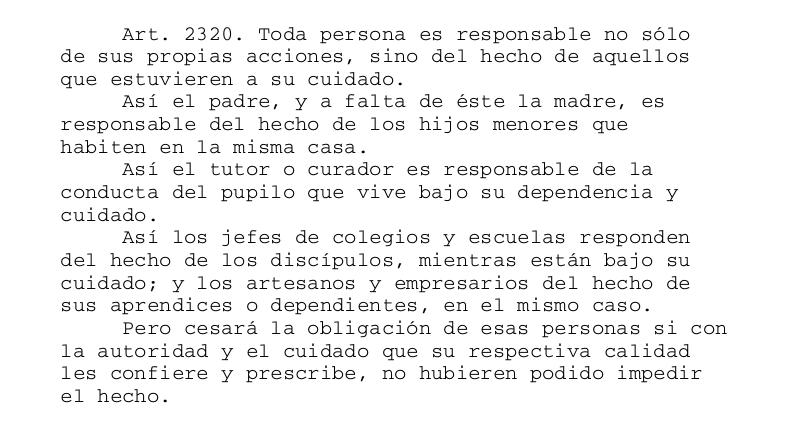
\includegraphics{2320.png?raw=true}
            \caption{Alt text}
            \end{figure}

            \begin{itemize}
            \item
              ocasionados por delito o cuasidelito penales y civiles

              art. 58 inc. 2º CPP relacionado con el art. 2314. Por las
              personas jurídicas responden los que hubieren intervenido
              en el acto punible, sin perjuicio de la responsabilidad
              civil que las afecte.

              art. 2314 El que ha cometido un delito o cuasidelito que
              ha inferido daño a otro, es obligado a la indemnización;
              sin perjuicio de la pena que le impongan las leyes por el
              delito o cuasidelito.
            \item
              ocasionado por delito o cuasidelitos exclusivamente
              civiles

              Se aplica el art. 2314 El que ha cometido un delito o
              cuasidelito que ha inferido daño a otro, es obligado a la
              indemnización; sin perjuicio de la pena que le impongan
              las leyes por el delito o cuasidelito.
            \end{itemize}
          \end{itemize}
        \end{itemize}
      \end{itemize}
    \end{itemize}
  \end{itemize}
\end{itemize}

\hypertarget{objeto-del-derecho}{%
\section{4. Objeto del Derecho}\label{objeto-del-derecho}}

\begin{itemize}
\item
  Bienes

  Son los que, pudiendo procurar al hombre una utilidad, es susceptible
  de apropiación por los particulares

  \begin{itemize}
  \tightlist
  \item
    Clasificación

    \begin{itemize}
    \item
      Corporales

      Son los que tienen existencia real y pueden ser percibidos por los
      sentidos.

      \begin{itemize}
      \item
        muebles

        Por naturaleza = que pueden transportarse de un lugar a otro,
        sea por una fuera externa o por sí mismos

        por anticipación = los que unidos a un inmuebles se consideran
        muebles para efectos de constituir derechos sobre ellos
      \item
        inmuebles

        por naturaleza = no pueden transportarse de un lugar a otro

        por adherencia = m. por naturaleza, se reputan inmuebles por
        estar \textbf{permanentemente adheridos}

        por destinación = m. por naturaleza, \textbf{permanentemente
        destinados al uso, cultivo o beneficio} de un inmueble
      \end{itemize}
    \item
      Incorporales

      Consisten en meros derechos

      \begin{itemize}
      \item
        Derechos reales

        sobre una cosa sin respecto a determinada persona, acciones
        reales
      \item
        Derechos personales

        solo pueden reclamarse de ciertas personas que por un
        \textbf{hecho suyo} o la \textbf{sola disposición de la ley} han
        contraído las obligaciones correlativas, acciones personales
      \end{itemize}
    \item
      Divisibles e Indivisibles

      atendiendo a si su división afecta su utilidad
    \item
      Consumibles e Inconsumibles

      conforme a si perecen o no con su primer uso al menos para su
      dueño
    \item
      Fungibles y no fungibles

      conforme a si tienen o no el mismo poder liberatorio
    \item
      De consumo y de medios de producción

      si satisfacen directa e inmediatamente las necesidades de las
      personas o si tiene por finalidad la producción de otros bienes
    \item
      Principales y Accesorios

      si tienen una existencia por sí mismos o si necesariamente
      requieren la existencia de otro
    \item
      Singulares y Universales

      Conforme a si constituyen una unidad ya sea natural o artificial.
      Son universales aquellas que a pesar de conservar su
      individualidad, forman un todo al estar unidas por un vínculo de
      igual destino, recibiendo una denominación común
    \item
      Otros

      Bienes presentes y futuros

      comerciables e incomerciables

      apropiables e inapropiables

      privados y públicos
    \end{itemize}
  \end{itemize}
\item
  El dominio

  art. 582 es el derecho real en una cosa corporal, para gozar y
  disponer de ella arbitrariamente, no siendo contra ley o contra
  derecho ajeno. Sobre las cosas incorporales hay también una especie de
  propiedad.

  \begin{itemize}
  \tightlist
  \item
    características

    \begin{enumerate}
    \def\labelenumi{\arabic{enumi}.}
    \tightlist
    \item
      derecho real, amparado por la acción reivindicatoria
    \item
      absoluto, las más amplias facultades (usar, gozar y disponer)
    \item
      exclusivo y excluyente, impide que terceros limiten o coarten el
      ejercicio de sus facultades
    \item
      perpetuo
    \end{enumerate}
  \item
    limitaciones

    \begin{enumerate}
    \def\labelenumi{\arabic{enumi}.}
    \tightlist
    \item
      ley
    \item
      derecho ajeno
    \item
      expropiación por utilidad pública
    \item
      ordenanzas municipales
    \item
      servidumbres prediales
    \item
      servicios eléctricos
    \item
      sentencia judicial
    \item
      teoría del abuso del derecho
    \end{enumerate}
  \item
    clasificación

    \begin{itemize}
    \item
      Plena y nuda

      Es nuda cuando el dueño se desprende del uso o goce, conservando
      la facultad de disposición
    \item
      Absoluta o fiduciaria

      Es fiduciaria la que se encuentra sujeta a gravamen de pasar a
      otra persona por el hecho de la verificación de una condición
    \item
      Individual o copropiedad

      Es copropiedad aquella en que varias personas son titulares del
      derecho de dominio sobre una misma cosa
    \item
      Civil, minera, industrial, indígena

      conforme a que leyes se rige
    \end{itemize}
  \end{itemize}
\item
  Modos de Adquirir

  \begin{itemize}
  \item
    Concepto

    \begin{enumerate}
    \def\labelenumi{\arabic{enumi}.}
    \tightlist
    \item
      Modo de Adquirir = hechos materiales que la ley le atribuye la
      virtud de hacer nacer o traspasar el derecho de dominio
    \item
      Título = hecho o acto jurídico que habilita y sirve de
      justificación para la adquisición del dominio o derecho real
      respectivo.
    \end{enumerate}
  \item
    clasificación

    \begin{itemize}
    \item
      originarios y derivativos

      conforme a si existe o no una relación de causa y efecto entre el
      antecesor, nadie puede transferir más derechos de los que tiene.

      son originarios: ocupación, accesión y la prescripción

      son derivativos: tradición, SPCM
    \item
      a titulo singular y a titulo universal

      ocupación y accesión

      SPCM
    \item
      entre vivos o por causa de muerte

      por mortis causa la SPCM
    \item
      a titulo gratuito y a titulo oneroso

      la tradición puede ser a titulo oneroso como también a titulo
      gratuito
    \end{itemize}
  \item
    la ocupación

    es el modo de adquirir las cosas \textbf{que no pertenecen a nadie}
    y cuya adquisición \textbf{no está prohibida por las leyes chilenas
    o el Derecho Internacional}, mediante la \textbf{aprehensión
    material} de ellas, \textbf{con la intención de adquirirlas}
  \item
    la accesión

    es un modo de adquirir por el cual el dueño de una cosa pasa a serlo
    de lo que ella produce o de lo que se junta a ella

    \begin{itemize}
    \tightlist
    \item
      clasificación

      \begin{itemize}
      \tightlist
      \item
        accesión de frutos

        \begin{itemize}
        \item
          frutos

          toda emanación periódica de una cosa sin detrimento de la cosa
          productora. 1) periodicidad, 2) sin detrimento, 3) conforme a
          su estimación natural o económica.

          civiles = utilidades pecuniarias, terceros al dueño, virtud de
          contrato, por el uso y goce

          naturales = ya sea con o sin la ayuda industrial del hombre
        \item
          productos

          todo lo que se obtiene de la cosa aun cuando para obtenerlo
          produzca su detrimento, como sería la tala de un bosque para
          vender sus maderas.
        \end{itemize}
      \item
        accesión propiamente tal

        \begin{itemize}
        \item
          Inmueble a inmueble

          \begin{enumerate}
          \def\labelenumi{\arabic{enumi}.}
          \tightlist
          \item
            aluvión = aumento que recibe la ribera de la mar, rio o lago
            por el lento, imperceptible y definitivo retiro de las aguas
          \item
            avulsión = aquella parte del suelo que arrancada por una
            avenida u fuerza natural violenta, es transportada por el
            agua a un predio inferior
          \item
            cambio de cause del rio
          \item
            formación de una nueva isla
          \end{enumerate}
        \item
          mueble a inmueble

          edificación y plantación o siembra ejecutados en un inmueble,
          cuando los materiales, plantas o semillas pertenecen distintas
          que el dueño del suelo
        \item
          mueble a mueble

          adjunción = dos cosas pertenecientes a distintos dueños se
          junta a otra, pero de modo que pueden separarse y subsistir
          cada una después de separada, como un espejo que se pone en un
          marco ajeno.

          especificación = cuando de la materia perteneciente a una
          persona, hace otra persona una obra o artefacto cualquiera

          mezcla = cuando se juntan materias solidas o líquidas
          pertenecientes a diferentes dueños, de manera que es imposible
          separarlos.
        \end{itemize}
      \end{itemize}
    \end{itemize}
  \item
    la tradición

    es un modo de adquirir el dominio de las cosas y consiste en la
    entrega que el dueño hace de ellas a otro, habiendo por una parte la
    facultad e intención de transferir el dominio y por la otra la
    capacidad e intención de adquirirlo, lo que se dice respecto al
    dominio también se extiende a los otros derechos reales.

    \begin{itemize}
    \item
      Requisitos de la tradición

      \begin{itemize}
      \tightlist
      \item
        Capacidad del tradente y del adquirente
      \item
        Consentimiento
      \item
        TTD
      \item
        Entrega material
      \end{itemize}
    \item
      Tiene las ss. características:

      \begin{itemize}
      \tightlist
      \item
        es un MAD derivativo
      \item
        puede ser a título oneroso como gratuito
      \item
        por RG es a título singular, pero puede ser a título universal
        también
      \item
        opera entre vivos
      \item
        es una convención que extingue obligaciones
      \item
        es un MAD y demás derechos reales
      \item
        sobre bienes corporales como incorporales
      \end{itemize}
    \item
      época de pedir la tradición

      RG inmediatamente, excepción:

      \begin{enumerate}
      \def\labelenumi{\arabic{enumi}.}
      \tightlist
      \item
        titulo condicional
      \item
        existencia de plazo para el pago
      \item
        cuando ha intervenido decreto judicial en contrario
      \end{enumerate}
    \item
      Diferencia entre entrega y tradición:

      \begin{itemize}
      \tightlist
      \item
        la entrega se refiere a la entrega \textbf{material} de una cosa
        a manos de otra persona
      \item
        la tradición implica la entrega (como elemento material),
        \emph{más} un elemento intencional, el cual, es el
        \textbf{título traslaticio de dominio}
      \end{itemize}
    \item
      título

      es el hecho o acto jurídico que sirve de antecedente para la
      adquisición. De el solo nacen derechos personales para exigir la
      transferencia del dominio.
    \item
      función de la inscripción en el registro del CBR

      \begin{enumerate}
      \def\labelenumi{\arabic{enumi}.}
      \tightlist
      \item
        tradición, como MAD = única forma de realizar la tradición de
        inmuebles y de los derechos reales constituidos en ellos, con
        excepción del dº real de herencia y servidumbres
      \item
        como formalidad de publicidad = ejemp. sentencia que declara la
        prescripción adquisitiva, renuncia de un dº real, resolución de
        interdicción provisoria o definitiva, resolución que confiere el
        beneficio de separación, gravamen sobre un inmueble, prohibición
        embargo o retención judicial legal o convencional
      \item
        requisito de garantía y prueba de la posesión de los bienes
        inmuebles = la posesión cesa por la cancelación de la
        inscripción (voluntad de las partes, nueva inscripción, decreto
        judicial)
      \item
        mantener la historia de la propiedad raíz
      \item
        solemnidad = casos de donaciones entre vivos, fideicomisos sobre
        inmuebles, usufructos sobre inmuebles, para la validez de censo
        e hipoteca, constitución de uso o habitación.
      \end{enumerate}
    \item
      títulos que se \textbf{deben} inscribir

      \begin{enumerate}
      \def\labelenumi{\arabic{enumi}.}
      \tightlist
      \item
        títulos traslaticios de dominio de los bienes inmuebles
      \item
        la constitución de los fideicomisos que comprendan o afecten
        bienes
      \item
        renuncia de alguno de los anteriores
      \item
        decretos de interdicción provisoria y definitiva, de
        rehabilitación del disipador y demente
      \end{enumerate}
    \item
      títulos que \textbf{pueden} inscribirse

      \begin{enumerate}
      \def\labelenumi{\arabic{enumi}.}
      \tightlist
      \item
        toda condición suspensiva o resolutoria del dominio de bienes
        inmuebles o de otros dº reales constituidos sobre ellos
      \item
        todo gravamen impuesto que no sea los 2 números anteriores, como
        servidumbres y arrendamiento u otro que sea permitida su
        inscripción
      \item
        todo impedimento o prohibición referente a un inmueble, sea
        convencional, legal o judicial como el embargo.
      \end{enumerate}
    \item
      Tradición de los derechos personales:

      En general, se realizan por la entrega del título del cedente al
      cesionario. La cual puede ser de tres tipos:

      \begin{itemize}
      \tightlist
      \item
        en nominativo: aceptado o notificado al deudor. Se encuentra
        regulado en el CC
      \item
        a la orden: efectuándose mediante el endoso. CdeCom.
      \item
        al portador: por la entrega del título. CdeCom.
      \end{itemize}
    \item
      La posesión

      es la tenencia de una cosa determinada con ánimo de señor y dueño,
      sea que el dueño o quien se da por tal tenga la cosa por sí misma,
      o por otra persona que la tenga en lugar y a nombre de él. El
      poseedor es reputado dueño mientras otra persona no justifica
      serlo.

      \begin{itemize}
      \tightlist
      \item
        Elementos:

        \begin{itemize}
        \tightlist
        \item
          tenencia
        \item
          cosa determinada
        \item
          ánimo de señor o dueño
        \end{itemize}
      \item
        Importancia:

        \begin{itemize}
        \tightlist
        \item
          se presume dueño
        \item
          acción publiciana (buena fe)
        \item
          sobre inmueble = acción posesoria
        \item
          prescripción adquisitiva
        \item
          buena fe = hace suyos los frutos
        \end{itemize}
      \item
        Diferencias con el dominio:

        \begin{itemize}
        \tightlist
        \item
          posesión = hecho; dominio = derecho
        \item
          posesión = acciones de corto tiempo; dominio = reivindicatoria
          mientras otro no adquiera la cosa por adquisitiva
        \item
          posesión = puede poseerse por varios títulos; dominio = solo
          puede adquirirse por 1 modo.
        \end{itemize}
      \item
        clasificación

        \begin{itemize}
        \item
          posesión regular / irregular

          la irregular carece de uno de los requisitos de la regular
          (los cuales son: a) justo título, b) buena fe inicial, c)
          tradición si es TTD)

          \begin{itemize}
          \item
            \begin{enumerate}
            \def\labelenumi{\alph{enumi})}
            \tightlist
            \item
              títulos injustos (``no es justo título'', art. 704)
            \end{enumerate}

            \begin{enumerate}
            \def\labelenumi{\arabic{enumi}.}
            \tightlist
            \item
              el falsificado
            \item
              el conferido por persona en calidad de mandatario o
              representante legal sin serlo
            \item
              el que adolece de vicio de nulidad
            \item
              el meramente putativo
            \end{enumerate}
          \item
            \begin{enumerate}
            \def\labelenumi{\alph{enumi})}
            \setcounter{enumi}{1}
            \tightlist
            \item
              buena fe
            \end{enumerate}

            conciencia de haberse adquirido el dominio de la cosa por
            medios legítimos, exentos de fraude o de todo otro vicio, la
            cual, por r.g. se presume

            \begin{itemize}
            \tightlist
            \item
              se presume la mala fe

              \begin{enumerate}
              \def\labelenumi{\arabic{enumi}.}
              \tightlist
              \item
                error de derecho (posesión)
              \item
                título de mera tenencia
              \item
                cuando se ha ocultado la verdadera muerte o existencia
                respecto de la posesión de los bienes del desaparecido
              \item
                al contestar la demanda
              \end{enumerate}
            \end{itemize}
          \item
            \begin{enumerate}
            \def\labelenumi{\alph{enumi})}
            \setcounter{enumi}{2}
            \tightlist
            \item
              TTD
            \end{enumerate}

            Cuando se trate de la tradición, se exige que exista un
            título traslaticio de dominio, el cual consta la voluntad de
            las partes.
          \end{itemize}
        \item
          posesión viciosa / útil

          es viciosa la violenta o clandestina y no permiten prescribir
        \item
          posesión continua / interrumpida

          es continua la que no ha sido perdida, impedida o desconocida
        \end{itemize}
      \item
        adquisición, conservación y perdida

        \begin{itemize}
        \item
          muebles

          adquisición = corpus y animus (capaces)

          conservación = basta el animus

          perdida = se puede perder por falta de uno u otro
          (\emph{corpus} = otro se apodera con animo de hacerla suya,
          imposible su ejercicio, se arrojan al mar, se pierden
          materialmente y no están bajo poder), (\emph{animus} =
          constituto posesorio), (\emph{corpus y animus} = cuando se
          enajena la cosa por tradición o se abandona para que la haga
          suya el primer ocupante)
        \item
          inmuebles no inscritos

          art. 729, al igual que los bienes muebles, sin perjuicio que
          dicho art. señala que si alguien pretendiéndose dueño se
          apodera violenta o clandestinamente de un inmueble cuyo título
          no está inscrito, el que tenía la posesión la pierde.
          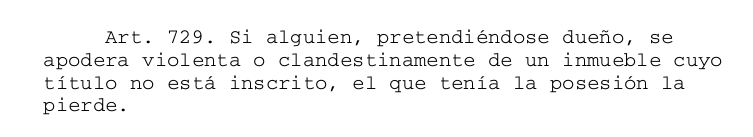
\includegraphics{729.png}
        \item
          inmuebles inscritos

          \begin{itemize}
          \item
            adquisición

            \begin{enumerate}
            \def\labelenumi{\arabic{enumi}.}
            \tightlist
            \item
              por título constitutivo
            \item
              por título traslaticio
            \end{enumerate}
          \item
            conservación

            se conserva mientras la inscripción no se cancele
          \item
            pérdida

            solamente por la \textbf{cancelación} de la inscripción, la
            que, puede ocurrir por:

            \begin{enumerate}
            \def\labelenumi{\arabic{enumi}.}
            \tightlist
            \item
              voluntad de las partes
            \item
              decreto judicial
            \item
              por nueva inscripción (si el título es justo o injusto, se
              cancela la anterior, si es mero tenedor el que enajena, la
              mayoría de la doctrina señala que cancela la anterior)
            \end{enumerate}
          \end{itemize}
        \end{itemize}
      \end{itemize}
    \end{itemize}
  \item
    la prescripción (\emph{adquisitiva})

    MAD de las cosas ajenas por haberse poseído las cosas durante un
    cierto lapso de tiempo y concurriendo los demás requisitos legales.

    \begin{itemize}
    \tightlist
    \item
      Elementos:

      \begin{itemize}
      \tightlist
      \item
        posesión
      \item
        títular inactivo
      \item
        trascurso de un lapso de tiempo
      \end{itemize}
    \item
      reglas comunes a la prescripción

      \begin{enumerate}
      \def\labelenumi{\arabic{enumi}.}
      \tightlist
      \item
        debe ser alegada, salvo acción penal, pena, prescripción del
        título ejecutivo
      \item
        puede ser renunciada
      \item
        corre contra todo tipo de persona
      \item
        debe ser declarada por sentencia judicial
      \item
        se adquiere por todos los derechos, gravámenes y limitaciones
      \item
        opera retroactivamente.
      \end{enumerate}
    \item
      Casos que no procede prescripción adquisitiva:

      \begin{itemize}
      \tightlist
      \item
        Servidumbres discontinuas o continuas inaparentes
      \item
        Derechos personales
      \item
        Cosas incomerciables
      \item
        Los derechos que tienen los propietarios de servirse de las
        aguas de lluvia
      \end{itemize}
    \item
      Requisitos de procedencia prescripción adquisitiva

      \begin{itemize}
      \tightlist
      \item
        Cosa susceptible de adquisición por prescripción
      \item
        Posesión útil y continua (la posesión útil puede ser regular o
        irregular)
      \item
        Tiempo, regular = 2 años muebles y 5 inmuebles; irregular = 10
        años
      \end{itemize}
    \item
      Clases de Prescripción Adquisitiva:

      \begin{itemize}
      \tightlist
      \item
        ordinaria

        \begin{itemize}
        \tightlist
        \item
          posesión regular
        \item
          tiempo, 2 años muebles; 5 años inmuebles
        \item
          se suspende
        \end{itemize}
      \item
        extraordinaria

        \begin{itemize}
        \tightlist
        \item
          posesión irregular
        \item
          tiempo, 10 años
        \item
          no se suspende
        \end{itemize}
      \end{itemize}
    \item
      Efectos que produce la prescripción:

      \begin{itemize}
      \tightlist
      \item
        es un MAD
      \item
        confiere acción y excepción
      \item
        opera en forma retroactiva
      \end{itemize}
    \end{itemize}
  \end{itemize}
\item
  Acción reivindicatoria

  art. 889, o acción de dominio es la que tiene el dueño de una cosa
  singular, de que no está en posesión, para que el poseedor de ella sea
  condenado a restituírsela.

  \begin{itemize}
  \item
    pretensión

    Que se le reconozca su dominio y que se ordene, por parte del juez,
    al que se encuentra poseyendo la cosa, que lo restituya en la
    posesión perdida.
  \item
    procedimiento judicial

    \begin{enumerate}
    \def\labelenumi{\arabic{enumi}.}
    \tightlist
    \item
      juicio de lato conocimiento, procedimiento ordinario
    \item
      si es mueble, será competente el juez de letras del domicilio del
      demandado
    \item
      si es inmueble, será el juez de letras del lugar en que se
      encuentra el inmueble.
    \end{enumerate}
  \item
    efectos

    \textbf{restituciones mutuas} = vencido restituir la cosa y los
    frutos, respondiendo de los deterioros y pérdidas, siendo obligado
    el vencedor en abonar las mejoras y gastos.
  \item
    cosas que pueden ser reinvindicables

    RG todas las cosas, muebles e inmuebles, corporales e incorporales.
    Salvo:

    \begin{enumerate}
    \def\labelenumi{\arabic{enumi}.}
    \tightlist
    \item
      cosas compradas en feria, tienda, almacén u otro establecimiento
      industrial en que se vendan cosas muebles de la misma clase.
      Deberá reembolsar al poseedor lo que haya dado por ella y lo que
      haya gastado en repararla y mejorarla
    \item
      solamente cosas singulares y universalidades de hecho. No se
      pueden reivindicar las universalidades de derecho.
    \item
      la herencia se reivindica por una acción especial denominada
      ``acción de petición de herencia''. Se diferencia con la
      reivindicatoria en que no puede accionar indistintamente, debe ser
      en contra del heredero putativo u otro título.
    \end{enumerate}

    \begin{itemize}
    \tightlist
    \item
      Reivindicación de una cuota determinada pro indiviso, de una cosa
      singular:

      \begin{itemize}
      \tightlist
      \item
        Cuota debe ser determinada
      \item
        Cosa singular proindiviso
      \end{itemize}
    \item
      Titulares de la acción reivindicatoria:

      \begin{itemize}
      \tightlist
      \item
        propietario
      \item
        comprador de una cosa a quien no se le ha hecho tradición no
        puede reivindicar
      \item
        pleno o nudo propietario
      \item
        absoluto o fiduciario
      \item
        copropietario por su cuota
      \end{itemize}
    \item
      Contra quien se puede reivindicar?

      \begin{itemize}
      \tightlist
      \item
        actual poseedor
      \item
        poseedor que haya dejado de serlo

        \begin{itemize}
        \item
          \begin{enumerate}
          \def\labelenumi{\alph{enumi})}
          \tightlist
          \item
            restitución de todo lo que haya recibido por ella = si se ha
            hecho imposible o difícil persecución
          \end{enumerate}
        \item
          \begin{enumerate}
          \def\labelenumi{\alph{enumi})}
          \setcounter{enumi}{1}
          \tightlist
          \item
            indemnización de todo perjuicio = si se enajenó a sabiendas
          \end{enumerate}
        \end{itemize}
      \item
        El injusto detentador
      \end{itemize}
    \end{itemize}
  \item
    acción publiciana

    Art. 894 se concede la misma acción (reivindicatoria) aun que no se
    pruebe el dominio, al que ha perdido la posesión regular de la cosa,
    y se hallaba en el caso de poderla ganar por prescripción, pero no
    contra el verdadero dueño ni contra quien lo posea con igual o mejor
    derecho.

    \begin{itemize}
    \item
      prueba

      \begin{enumerate}
      \def\labelenumi{\arabic{enumi}.}
      \tightlist
      \item
        el poseedor se reputa dueño
      \item
        fisco se reputa dueño de aquellas tierras que carecen de uno
      \item
        que el dominio se adquirió por algún modo (ocupación, accesión,
        prescripción, tradición, remontándose hasta un MAD originario,
        10 años)
      \item
        que el demandado se encuentra en posesión de la cosa
      \item
        determinación e identificación de la cosa
      \end{enumerate}
    \item
      prestaciones mutuas

      terminado el juicio reivindicatorio, vencido el demandado, se da
      lugar a las prestaciones mutuas

      consiste en los hechos y pagos que el poseedor vencido debe hacer
      en favor del reivindicante y que éste a su vez debe hacer en favor
      del poseedor.

      estas reglas se aplican también la \textbf{nulidad, accesión de
      mueble a inmueble y ala acción de petición de herencia}.

      \begin{itemize}
      \tightlist
      \item
        prestaciones del poseedor vencido a favor del reivindicante

        \begin{itemize}
        \item
          restitución de la cosa

          dentro del plazo que señale el juez, comprende la cosa misma,
          las cosas inmuebles por adherencia o destinación, cuestiones
          accesorias que hayan sido comprendidas en la demanda y
          sentencia y los títulos que conciernen a la cosa. Al momento
          de la entrega es conveniente que se haga ante un ministro de
          fe para que deje constancia del estado de la cosa.
        \item
          indemnización deterioros

          no se es responsable de los deterioros que por su hecho o
          culpa sufra la cosa (a menos que se haya aprovechado de ellos,
          haciéndose más rico), mientras no conteste la demanda. Por lo
          que, se entiende en buena fe hasta el momento de la
          contestación.
        \item
          restitución de frutos

          poseedor de mala fe debe restituir los frutos civiles y
          naturales que el dueño hubiera podido percibir con la mediana
          inteligencia y actividad. Pagando su valor en caso que no
          existan. Estos se restituyen líquidos, descontando los gastos
          ordinarios invertidos para producirlos
        \item
          gastos del pleito, conservación y custodia

          si es condenado en costas. Poseedor de mala fe deberá pagar
          los gastos de conservación y custodia en caso de medida
          precautoria de secuestro.
        \end{itemize}
      \item
        Prestaciones del reivindicante en favor del poseedor vencido

        \begin{enumerate}
        \def\labelenumi{\arabic{enumi}.}
        \tightlist
        \item
          gastos \textbf{ordinarios de producción de los frutos}
        \item
          \textbf{abono de expensas y mejoras}.

          \begin{itemize}
          \tightlist
          \item
            Necesarios (siempre)
          \item
            las no necesarias pueden ser útiles (aumentando el valor
            venal de la cosa) + buena fe, podrá pagar lo que las obras
            valgan o pagar lo que la cosa valiere más al momento de su
            restitución. Si estaba de mala fe, no tiene derecho a que se
            le abonen, pero puede llevarse los materiales que puedan
            separarse sin detrimento de la cosa
          \item
            Voluptuarias (no aumentan el valor o es insignificante), no
            se pagan pero da derecho a retiro por parte del vencido si
            se pueden separar sin detrimento de la cosa.
          \end{itemize}
        \end{enumerate}
      \end{itemize}
    \end{itemize}
  \end{itemize}
\item
  Acciones posesorias

  son las que tienen por objeto \emph{conservar} o \emph{recuperar} la
  posesión de \emph{bienes raíces} o de derechos reales constituidos en
  \emph{ellos}

  \begin{itemize}
  \tightlist
  \item
    prueba de la posesión

    \begin{enumerate}
    \def\labelenumi{\arabic{enumi}.}
    \tightlist
    \item
      dº reales inscritos = por la inscripción
    \item
      dº reales no inscritos = por hechos positivos, lo mismo se aplica
      poseedor inscrito menos de 1 año, dos inscripciones, deslindes no
      son exactos
    \end{enumerate}
  \end{itemize}
\item
  querella de amparo

  es la que tiene por objeto conservar (que no se turbe, indemnice,
  garantías)la posesión de bienes raíces o dº reales sobre ellos
\item
  querella de restitución

  es la que tiene por objeto recuperar (y ser indemnizado) la posesión
  de bienes raíces y dº reales sobre ellos.
\item
  querella de restablecimiento

  es la que tiene el poseedor y el mero tenedor que ha sido despojado
  violentamente de la posesión o mera tenencia de un inmueble, a fin de
  que se le restituya al estado que se encontraba. (6 meses)
\item
  Dº reales limitados o limitantes del dominio

  \begin{itemize}
  \item
    propiedad fiduciaria

    la que está sujeta al gravamen de pasar a otra persona, por el hecho
    de verificarse una condición

    \begin{itemize}
    \tightlist
    \item
      requisitos:

      \begin{itemize}
      \tightlist
      \item
        cosa susceptible de constituirse en fideicomiso (cosa mueble o
        inmueble, totalidad de una herencia, cuota determinada)
      \item
        concurrencia de: fideicomisario, propietario fiduciario y
        constituyente
      \item
        La existencia de una condición
      \end{itemize}
    \end{itemize}
  \item
    usufructo

    es un derecho real que consiste en la facultad de gozar de una cosa
    con cargo de conservar su forma y substancia, y de restituírsela a
    su dueño, si la cosa no es fungible, o con cargo de devolver igual
    cantidad y calidad del mismo genero, o de pagar su valor si es
    fungible

    Está constituido por tres elementos: cosa susceptible de usufructo,
    las personas que intervienen, el plazo.

    \begin{itemize}
    \tightlist
    \item
      características:

      \begin{itemize}
      \tightlist
      \item
        derecho real de goce
      \item
        principal
      \item
        mueble o inmueble
      \item
        usufructuario es mero tenedor
      \item
        temporal
      \item
        existencia de un plazo
      \item
        intrasmisible, puede ser transferible mientras no se lo haya
        prohibido
      \item
        debe recaer en cosa ajena
      \end{itemize}
    \item
      Fuentes del derecho real de usufructo:

      \begin{itemize}
      \tightlist
      \item
        ley
      \item
        testamento (en tal caso, solemne)
      \item
        acto entre vivos
      \item
        prescripción
      \item
        sentencia judicial (excepcional, en partición de bienes)
      \end{itemize}
    \item
      El cuasiusufructo:

      \begin{itemize}
      \tightlist
      \item
        es TTD
      \item
        cuasiusufructo tiene derecho a restitución de su crédito
        (usufructo tiene acción reivindicatoria)
      \item
        el género no perece
      \end{itemize}
    \item
      Efectos:

      \begin{itemize}
      \tightlist
      \item
        derechos del propietario:

        \begin{itemize}
        \tightlist
        \item
          usar y gozar la cosa
        \item
          administrar la cosa
        \item
          a arrendar y ceder el usufructo
        \item
          disponer de la cosa
        \end{itemize}
      \item
        obligaciones del usufructuario

        \begin{itemize}
        \tightlist
        \item
          previas

          \begin{itemize}
          \tightlist
          \item
            inventario y rendir caución
          \end{itemize}
        \item
          durante el usufructo

          \begin{itemize}
          \tightlist
          \item
            respetar los arriendos y demás cargas
          \item
            mantener la cosa y su substancia
          \item
            pagar expensas y mejoras
          \item
            si fue constituido por testamento, puede quedar obligado
            respecto a las deudas hereditarias
          \end{itemize}
        \end{itemize}
      \item
        derechos del nudo propietario

        \begin{itemize}
        \tightlist
        \item
          a los frutos pendientes al tiempo de la restitución
        \item
          indemnización de perjuicios y deterioros
        \item
          terminación anticipada
        \item
          acciones de dominio y acciones posesorias (si es sobre un
          inmueble)
        \end{itemize}
      \item
        obligaciones del nudo propietario

        \begin{itemize}
        \tightlist
        \item
          expensas extraordinarias mayores
        \end{itemize}
      \end{itemize}
    \item
      Extinción del usufructo:

      \begin{itemize}
      \tightlist
      \item
        llegada del plazo, cumplimiento condición
      \item
        muerte usufructuario
      \item
        resolución del derecho constituyente
      \item
        prescripción
      \item
        consolidación del usufructo con la nuda propiedad
      \item
        renuncia del usufructuario
      \item
        destrucción completa de la cosa sentencia judicial en los casos
        establecidos por ley
      \end{itemize}
    \end{itemize}
  \item
    servidumbre

    es el gravamen impuesto sobre un predio en utilidad de otro predio
    de distinto dueño

    \begin{itemize}
    \tightlist
    \item
      características:

      \begin{itemize}
      \tightlist
      \item
        es un gravamen
      \item
        derecho real
      \item
        inmueble
      \item
        accesorio
      \item
        perpetuo
      \item
        indivisible en su ejercicio
      \end{itemize}
    \item
      clasificación en cuanto a su naturaleza:

      \begin{itemize}
      \tightlist
      \item
        Aparentes e inaparentes
      \item
        Continuas y discontinuas
      \end{itemize}
    \end{itemize}
  \item
    uso o habitación

    es un derecho real que consiste generalmente en la facultad de gozar
    de una parte limitada de las utilidades y productos de una cosa. Si
    se refiere a una casa, y la utilidad de morar en ella, se llama
    derecho de habitación.

    \begin{itemize}
    \tightlist
    \item
      Características

      \begin{itemize}
      \tightlist
      \item
        derecho real
      \item
        personalísimos
      \item
        inembargables
      \item
        se constituyen e se extinguen como el usufructo
      \item
        se limitan a las necesidades del usuario (y su familia)
      \item
        usuario debe actuar como buen padre de familia \# 5.
        Obligaciones
      \end{itemize}
    \end{itemize}
  \end{itemize}
\item
  Concepto

  Es un vínculo jurídico entre personas determinadas, en cuya virtud una
  de ellas, denominada deudor, se encuentra para con la otra, llamada
  acreedor, en la necesidad de dar, hacer o no hacer una cosa.
  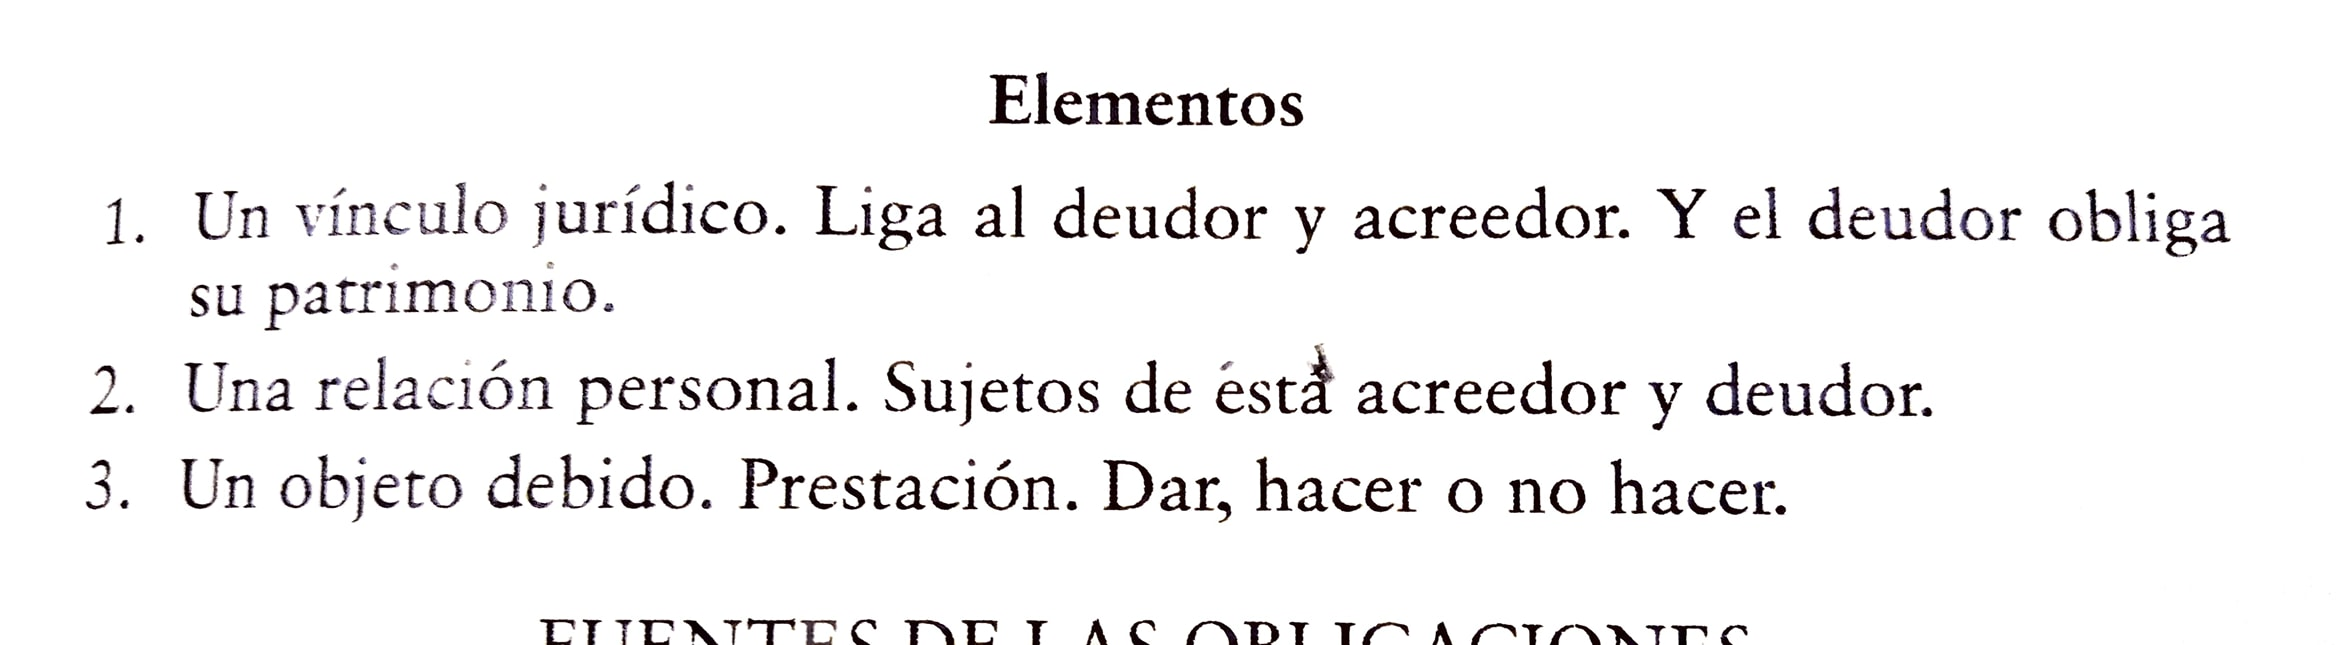
\includegraphics{elementos.jpeg}
\item
  Fuentes

  \begin{enumerate}
  \def\labelenumi{\arabic{enumi}.}
  \tightlist
  \item
    contrato
  \item
    cuasicontrato
  \item
    delito
  \item
    cuasidelito
  \item
    la ley
  \item
    para algunos, la declaración unilateral de voluntad
  \end{enumerate}
\item
  Clasificación

  \begin{itemize}
  \item
    Civiles y Naturales

    son civiles las que dan derecho para exigir su cumplimiento art.
    1470

    son naturales las que no dan derecho para exigir su cumplimiento
    pero que cumplidas, autorizan para retener lo que se ha dado o
    pagado en razón de ellas.

    \begin{itemize}
    \tightlist
    \item
      Señale los casos de obligación natural (art. 1470)

      \begin{enumerate}
      \def\labelenumi{\arabic{enumi}.}
      \tightlist
      \item
        las contraídas por los \textbf{incapaces relativos}
      \item
        las que proceden de \textbf{actos a que faltan solemnidades}
      \item
        obligaciones civiles \textbf{prescritas}
      \item
        las que no han sido reconocidas por \textbf{falta de prueba}
      \end{enumerate}
    \item
      Otros casos de oº naturales

      \begin{enumerate}
      \def\labelenumi{\arabic{enumi}.}
      \tightlist
      \item
        pago de intereses no estipulados en el mutuo
      \item
        pago de apuestas en que predomina la inteligencia
      \item
        multa en esponsales
      \item
        pago por objeto o causa ilícita a sabiendas
      \item
        en el beneficio de inventario cuando se paga más allá de lo
        recibido por herencia.
      \end{enumerate}
    \item
      efecto de las oº naturales

      \begin{enumerate}
      \def\labelenumi{\arabic{enumi}.}
      \tightlist
      \item
        autorizan a \emph{retener} lo pagado
      \item
        pueden ser \emph{novadas}
      \item
        pueden ser \emph{caucionadas}
      \item
        no se extinguen por sentencia
      \item
        no se puede alegar la excepción de cosa juzgada
      \end{enumerate}
    \end{itemize}
  \item
    Positivas y Negativas

    dependiendo si consisten en llevar a cabo una prestación o una
    abstención
  \item
    De especie o cuerpo cierto y de género

    dependiendo de su determinación, debiendo ser a lo menos determinado
    en su género.

    \begin{itemize}
    \tightlist
    \item
      efectos de especie o cuerpo cierto

      \begin{enumerate}
      \def\labelenumi{\arabic{enumi}.}
      \tightlist
      \item
        se satisface entregando precisamente la cosa
      \item
        está obligado a conservar la cosa
      \item
        debe emplearse una diligencia que puede estar graduada conforme
        a si beneficia al deudor, acreedor o ambos
      \item
        se extingue con la pérdida de la cosa
      \end{enumerate}
    \item
      efecto de género

      \begin{enumerate}
      \def\labelenumi{\arabic{enumi}.}
      \tightlist
      \item
        el acreedor no puede pedir determinadamente un individuo
      \item
        el deudor cumple entregando cualquier individuo del género
        determinado de una calidad a lo menos mediana
      \item
        el deudor puede destruir o enajenar las cosas genéricas,
        mientras subsistan otras para el cumplimiento de lo que se debe
      \item
        la perdida de algunas cosas no extingue la obligación, el género
        no perece
      \item
        no opera la teoría de los riesgos
      \end{enumerate}
    \end{itemize}
  \item
    De dar, hacer o no hacer

    Es de dar la que tiene por objeto \emph{transferir} el dominio o
    constituir un derecho real o la mera tenencia

    Es de hacer la que tiene por objeto la \emph{ejecución} de un hecho
    cualquiera, material o jurídico

    No hacer consiste en la \emph{abstención} de un hecho que, \emph{de
    otro modo sería lícito ejecutar}
  \item
    Objeto singular y objeto múltiple

    las de objeto múltiple a su vez se clasifican en

    \begin{itemize}
    \item
      de simple objeto múltiple

      se deben varias cosas copulativamente de modo que el deudor se
      libera prestándolas o ejecutándolas todas
    \item
      alternativas

      se deben \textbf{varias} cosas pero que la ejecución de una de
      ellas \emph{exonera} al deudor de la ejecución de las demás

      \begin{itemize}
      \tightlist
      \item
        características

        \begin{enumerate}
        \def\labelenumi{\arabic{enumi}.}
        \tightlist
        \item
          elección del deudor salvo estipulación en contrario
        \item
          acreedor no obligado a aceptar parte de una y parte de otra
        \item
          acreedor debe demandar en la alternativa en que se deben
        \item
          si son varios se debe hacer la elección de consuno
        \item
          pérdida parcial y culpable y la elección es del acreedor,
          puede pedir a su arbitrio el precio de la cosa perdida más
          indemnización u otra de las cosas que se debían en alternativa
          (sin indemnización)
        \item
          las cosas se deben bajo la condición de que sean elegidos
        \item
          será mueble o inmueble según el objeto para el pago
        \end{enumerate}
      \end{itemize}
    \item
      facultativas

      son aquellas que se debe \textbf{una} cosa determinada pero
      \emph{concediéndose} al deudor la facultad de pagar con esta cosa
      o con otra que se designa.

      \begin{itemize}
      \tightlist
      \item
        efectos

        \begin{itemize}
        \tightlist
        \item
          acreedor sólo puede pedir la cosa debida
        \item
          dación en pago pactada anticipadamente
        \item
          puede ser mueble o inmueble
        \item
          en caso de duda se tiene por alternativa
        \end{itemize}
      \end{itemize}
    \end{itemize}
  \item
    Con unidad de sujetos o pluralidad de sujetos

    con unidad de sujeto solo existe un acreedor y un deudor, lo que no
    exige mucho análisis, a diferencia de pluralidad sujetos que se
    pueden clasificar en:

    \begin{itemize}
    \item
      simplemente conjuntas o mancomunadas

      son aquellas en que cada uno de los deudores es obligado solamente
      a su parte o cuota en la deuda y cada uno de los acreedores sólo
      tiene derecho para demandar su parte o cuota en el crédito.

      consecuencias = existe una pluralidad de prestaciones y vínculos
      independientes entre si, el objeto es física y moralmente
      divisible, cada deudor solo obligado al pago de su cuota y cada
      acreedor a su parte del crédito, la cuota del deudor insolvente no
      grava a sus codeudores, la interrupción de uno no afecta a los
      demás, la culta tampoco, excepciones personales solo por sus
      titulares, mora de uno no afecta los demás, nulidad de uno no
      afecta a los otros.
    \item
      solidarias

      aquellas en que hay varios deudores o acreedores y la prestación
      recae sobre un objeto divisible, pero por disposición de la ley o
      expresa declaración de voluntad, cada acreedor puede demandar y
      cada deudor debe satisfacer el total de la obligación de manera
      que el pago efectuado por un deudor a cualquiera de los acreedores
      extingue la obligación respecto a todos.

      puede tener por fuente el testamento

      solidaridad activa = cada acreedor puede demandar el total al
      deudor, el cual puede pagar a cualquiera de los acreedores con tal
      que no haya sido demandado por uno de ellos, pago que extingue la
      obligación respecto a todos, la interrupción de la prescripción
      aprovecha a los demás.

      solidaridad pasiva = acreedor puede demandar a cualquiera de los
      deudores el total, el cual extingue respecto a todos los deudores
      si es pagada, la interrupción de la prescripción perjudica a
      todos, la mora de uno afecta a todos, la perdida de la cosa por
      uno hace solidarios en el precio y la indemnización la responde el
      culpable, cada deudor puede interponer las excepciones reales
      personales o mixtas.

      Extinción de la solidaridad:

      \begin{itemize}
      \tightlist
      \item
        muerte
      \item
        renuncia del acreedor
      \end{itemize}
    \item
      indivisibles

      aquellas en que la prestación recae sobre un objeto que no es
      susceptible de división física, intelectual o de cuota.

      \begin{itemize}
      \tightlist
      \item
        activa

        \begin{enumerate}
        \def\labelenumi{\arabic{enumi}.}
        \tightlist
        \item
          cada acreedor puede pedir el total
        \item
          se transmite a los herederos
        \item
          el pago hecho a uno de los acreedores extingue la obligación
          respecto de los demás
        \item
          la interrupción de la prescripción de uno beneficia a los
          demás
        \item
          un acreedor no puede sin el consentimiento de los otros
          remitir la deuda o recibir el precio en vez de la cosa
        \end{enumerate}
      \item
        pasiva

        \begin{enumerate}
        \def\labelenumi{\arabic{enumi}.}
        \tightlist
        \item
          se transmite a los herederos
        \item
          pago hecho por uno extingue la obligación de los demás
        \item
          la interrupción de la prescripción contra uno beneficia a los
          demás
        \item
          demandado puede pedir plazo para entenderse con los demás,
          salvo que solamente él pueda cumplirla
        \item
          la de indemnizar los perjuicios es divisible en la parte que a
          cada uno quepa
        \item
          las relaciones internas de los codeudores se rigen por las
          reglas de las oº simplemente conjuntas.
        \end{enumerate}
      \item
        indivisibilidad de pago art. 1526

        \begin{enumerate}
        \def\labelenumi{\arabic{enumi}.}
        \tightlist
        \item
          acción hipotecaria
        \item
          deuda de especie o cuerpo cierto
        \item
          codeudor cuyo hecho o culpa hizo imposible cumplimiento
        \item
          obligación de pagar exclusivamente deuda hereditaria o
          testamentaria
        \item
          si se debe una cosa cuya división ocasione grave perjuicio al
          acreedor
        \item
          cuando la obligación es alternativa.
        \end{enumerate}
      \end{itemize}
    \end{itemize}
  \item
    Obligaciones principales y accesorias

    principales = las que tienen una existencia propia, capaz de
    subsistir por si mismas

    accesorias = son las que no pueden subsistir por sí solas y suponen
    una oº principal a que acceden y garantizan
  \item
    de ejecución instantánea y de tracto sucesivo

    ejecución instantánea = la prestación por su naturaleza se cumple en
    un solo acto

    tracto sucesivo = se cumple continuamente en el tiempo
  \item
    puras y simples y sujetas a modalidad

    puras y simples = son aquellas que producen sus efectos desde que se
    contraen para siempre y sin limitaciones

    sujetas a modalidades = aquellas cuyo efectos regulares se alteran
    por la introducción de ciertas cláusulas que afectan el nacimiento,
    ejercicio, extinción o manera de ejercitar los derechos
    consiguientes.

    \begin{itemize}
    \item
      condición

      hecho futuro e incierto del cual depende el nacimiento o la
      extinción de un derecho. Pueden ser expresas o tácitas,
      determinadas o indeterminadas (si el hecho ha de suceder se
      desconoce cuando), positivas (consisten en acontecer algo),
      negativas (no acontezca algo) físicamente imposible (contraria a
      las leyes naturales) moralmente imposible (prohibida por las
      leyes, buenas costumbres u el orden público)

      \begin{itemize}
      \item
        suspensiva

        aquellas que mientras no se cumplan \emph{suspenden el
        nacimiento} de un derecho

        \begin{enumerate}
        \def\labelenumi{\arabic{enumi}.}
        \tightlist
        \item
          positiva, física o moralmente imposible = fallida
        \item
          negativa, moralmente imposible = fallida
        \item
          negativa, físicamente imposible = no escrita
        \end{enumerate}

        \begin{itemize}
        \item
          efectos mientras está pendiente

          \begin{enumerate}
          \def\labelenumi{\arabic{enumi}.}
          \tightlist
          \item
            acreedor tiene un derecho en germen al cual puede ser
            trasmitido, impetrar medidas conservativas y de efecto
            retroactivo
          \item
            no se puede exigir su cumplimiento (si paga puede repetirse)
          \item
            no tiene derecho a los frutos
          \item
            no tiene acción de partición
          \item
            tiene derecho al precio y perjuicios si se pierde la cosa
            por culpa del deudor
          \item
            no corre la prescripción
          \end{enumerate}
        \item
          fallida

          nunca ha existido obligación
        \item
          cumplida

          \begin{enumerate}
          \def\labelenumi{\arabic{enumi}.}
          \tightlist
          \item
            nace el derecho y la obligación correlativa
          \item
            opera la prescripción y la compensación
          \item
            opera la retroactividad
          \end{enumerate}
        \item
          casos en que opera retroactivamente

          \begin{enumerate}
          \def\labelenumi{\arabic{enumi}.}
          \tightlist
          \item
            derechos deferidos a la criatura que está por nacer
          \item
            hipoteca bajo condición
          \item
            venta de cosa ajena
          \item
            tradición de cosa ajena
          \end{enumerate}
        \item
          casos en que no opera retroactivamente

          \begin{enumerate}
          \def\labelenumi{\arabic{enumi}.}
          \tightlist
          \item
            respecto de los frutos
          \item
            en el caso que se haya enajenado a tercero de buena fe
          \item
            riesgo es del deudor, salvo mala fe
          \item
            contratos de tracto sucesivo
          \end{enumerate}
        \end{itemize}
      \item
        resolutoria

        la que con su cumplimiento extingue un derecho

        \begin{enumerate}
        \def\labelenumi{\arabic{enumi}.}
        \tightlist
        \item
          positiva, física o moralmente imposible = no escrita
        \item
          negativa, física o moralmente imposible = no escrita
        \end{enumerate}

        \begin{itemize}
        \item
          ordinaria

          es la que consiste en un hecho futuro e incierto del cual
          depende la extinción de un derecho, \emph{no consistiendo en
          el incumplimiento de una obligación} - opera de pleno derecho.
        \item
          CRT

          es la que va envuelta en todo contrato bilateral y consiste en
          el \textbf{no cumplimiento por parte de uno de los
          contratantes} de lo pactado - dando al contratante diligente
          un dº opcional que puede ser el cumplimiento forzado de la
          obligación o su resolución y en ambos casos con indemnización
          de perjuicios.
        \item
          pacto comisorio

          simple: es la CRT expresamente estipulada, la cual confiere a
          la parte diligente que haya cumplido o se encuentre llana a
          cumplirla, los mismos derechos señalados anteriormente.

          calificado o ipso facto: es aquel en que se estipula que si no
          se cumple se resolverá ipso facto el contrato. En la CV da
          derecho al deudor en pagar dentro de las 24 hrs, en los otros
          no existe este derecho para poder enervar la acción
          resolutoria.
        \item
          efectos

          \begin{enumerate}
          \def\labelenumi{\arabic{enumi}.}
          \tightlist
          \item
            pendiente = nace el dº con todos sus atributos, sujeto al
            evento de extinguirse por la condición
          \item
            fallida = se consolida definitivamente el dº y el acto se
            reputa puro y simple
          \item
            cumplida = se extingue el dº y desaparece la oº.

            \begin{itemize}
            \tightlist
            \item
              \emph{entre las partes} = restitución de la cosa, conserva
              los frutos (salvo la ley o estipulación en contra)
            \item
              \emph{respecto de terceros} = si es mueble no dará dº a
              reivindicarla contra 3º de buena fe, si es inmueble, solo
              podrá reivindicarla cuando la condición constaba en el
              título respectivo, inscrito u otorgado por escritura
              pública.
            \end{itemize}
          \end{enumerate}
        \item
          acción resolutoria

          es la que nace de la CRT y del pacto comisorio para pedir la
          resolución del contrato por el incumplimiento de las oº
          contraídas. prescribe en los 5 años (CRT) y 4 años (o menos si
          emana del pacto comisorio)
        \end{itemize}
      \item
        cumplimiento de las condiciones

        \begin{enumerate}
        \def\labelenumi{\arabic{enumi}.}
        \tightlist
        \item
          del modo en que las partes haya entendido que lo fuese
        \item
          se presume que dicho modo es el más racional
        \item
          literalmente en la forma convenida y no por equivalencia
        \item
          totalmente
        \item
          dentro de la época fijada (si es determinada)
        \item
          aún después de la muerte de los contratantes.
        \end{enumerate}
      \end{itemize}
    \item
      plazo

      es un hecho futuro y cierto del cual depende la exigibilidad o la
      extinción de un derecho y de sus obligaciones correlativas. el
      plazo cuando es resolutorio extingue la oº de pleno dº.

      \begin{itemize}
      \tightlist
      \item
        efectos

        \begin{itemize}
        \tightlist
        \item
          pendiente

          \begin{enumerate}
          \def\labelenumi{\arabic{enumi}.}
          \tightlist
          \item
            no puede exigirse el cumplimiento
          \item
            no corre prescripción
          \item
            no corre compensación
          \end{enumerate}
        \item
          cumplido

          \begin{enumerate}
          \def\labelenumi{\arabic{enumi}.}
          \tightlist
          \item
            la obligación se hace exigible
          \item
            constituye en mora al deudor
          \end{enumerate}
        \end{itemize}
      \item
        extinción del plazo

        \begin{enumerate}
        \def\labelenumi{\arabic{enumi}.}
        \tightlist
        \item
          cumplimiento
        \item
          renuncia
        \item
          caducidad, por procedimiento concursal o la insolvencia o por
          la disminución o extinción de cauciones.
        \end{enumerate}
      \end{itemize}
    \item
      modo

      consiste en un gravamen o carga impuesta por el acreedor al deudor
      para que tenga por suyo el objeto de la oº debiendo aplicarlo a un
      fin especial o sujetarse a un determinado gravamen.

      \begin{itemize}
      \tightlist
      \item
        efectos

        \begin{enumerate}
        \def\labelenumi{\arabic{enumi}.}
        \tightlist
        \item
          no suspende la adquisición de la cosa
        \item
          el derecho no se extingue por el incumplimiento del modo
          (salvo que consista en una condición, contratos bilaterales)
        \item
          si el modo es imposible se tiene por no escrito
        \item
          si es imposible en la forma prevista y sin culpa del deudor se
          cumple por equivalencia.
        \item
          si se hace imposible sin culpa del deudor, la oº se reputa
          pura y simple.
        \end{enumerate}
      \end{itemize}
    \end{itemize}
  \end{itemize}
\item
  Efectos de las Obligaciones

  \begin{itemize}
  \item
    concepto

    son los dº que la ley confiere al acreedor para obtener el
    cumplimiento exacto, íntegro y oportuno de la oº, cuando éste no la
    cumple en todo o en parte o esta en mora de cumplirla.
  \item
    medios que tiene el acreedor para obtener el cumplimiento de la oº

    \begin{enumerate}
    \def\labelenumi{\arabic{enumi}.}
    \tightlist
    \item
      el dº de pedir el \textbf{cumplimiento forzado} de la oº
    \item
      el derecho a la \textbf{indemnización de perjuicios}
    \item
      los \textbf{derechos auxiliares} del acreedor (medidas
      conservativas, la acción subrogatoria, la acción pauliana y el
      beneficio de separación)
    \end{enumerate}
  \item
    \begin{enumerate}
    \def\labelenumi{\arabic{enumi}.}
    \tightlist
    \item
      De la ejecución forzada de la oº

      \begin{enumerate}
      \def\labelenumii{\arabic{enumii}.}
      \tightlist
      \item
        dº de prenda general de los acreedores, de perseguir la
        ejecución de una oº sobre todos los bienes raíces o muebles del
        deudor, presentes o futuros, excepto los inembargables y las oº
        naturales
      \item
        los acreedores podrán exigir que se vendan todos los bienes del
        deudor hasta concurrencia de sus créditos, intereses y costas,
        para que con el producto se les satisfaga íntegramente.
      \item
        para la ejecución forzada se requiere un título ejecutivo.
      \end{enumerate}

      \begin{itemize}
      \item
        oº de dar

        \begin{enumerate}
        \def\labelenumii{\arabic{enumii}.}
        \tightlist
        \item
          mediante el uso de la fuerza pública si se encuentra en poder
          del deudor
        \item
          si se trata de dinero, se remata los bienes embargados para el
          pago
        \item
          se requiere que sea deuda líquida o posible de liquidarse,
          conste en un título ejecutivo, actualmente exigible, no esté
          prescrita
        \end{enumerate}
      \item
        oº de hacer

        \begin{enumerate}
        \def\labelenumii{\arabic{enumii}.}
        \tightlist
        \item
          pedir que se apremie al deudor para la ejecución del hº
        \item
          que se autorice al acreedor para hacerlo ejecutar a expensas
          del deudor
        \item
          que el deudor le indemnice los perjuicios resultantes de la
          infracción del contrato
        \item
          se requiere que conste en un título ejecutivo, actualmente
          exigible, determinado o determinable (el hº), que no esté
          prescrito.
        \end{enumerate}
      \item
        oº de no hacer

        \begin{enumerate}
        \def\labelenumii{\arabic{enumii}.}
        \tightlist
        \item
          si puede destruirse lo hº y es necesario para el objeto que se
          tuvo en vista al contratar, puede ser compelido (el deudor) a
          la destrucción o autorizar al acreedor para proceder a su
          destrucción a expensas del deudor
        \item
          si no es necesaria puede cumplirse por equivalencia
        \item
          si la destrucción no es posible, se indemnizara perjuicios
        \item
          requiere: titulo ejecutivo, actualmente exigible, que se
          convierta en la destrucción de la obra, que no esté prescrita
        \end{enumerate}
      \item
        embargo

        Es la aprehensión real o simbólica de uno o más bienes del
        deudor por ministro de fe, por autorización judicial, para que
        con el producto de la realización se pague al acreedor su
        crédito.

        \begin{itemize}
        \tightlist
        \item
          como se realiza

          \begin{enumerate}
          \def\labelenumii{\arabic{enumii}.}
          \tightlist
          \item
            se verifica por la entrega real o simbólica a un depositario
            que designe el juez, aun que se mantengan en poder del
            deudor.
          \item
            si recae dineros, alhajas, especies preciosas o efectos
            públicos, deberá hacerse el depósito en el banco estado de
            chile a la orden del juez de la causa
          \item
            si recae sobre bienes raíces o derechos reales sobre ellos
            debe inscribirse en el CBR donde estén ubicados.
          \end{enumerate}
        \item
          efectos

          \begin{enumerate}
          \def\labelenumii{\arabic{enumii}.}
          \tightlist
          \item
            priva al deudor de la administración de los bienes
          \item
            priva al deudor de la facultad de disposición (pero no del
            dominio)
          \item
            habilita al acreedor para realizar los bienes embargados y
            pagarse con su producto
          \end{enumerate}
        \end{itemize}
      \item
        prelación de crédito

        consiste en un conjunto de reglas establecidas por la ley que
        determinan el orden y forma en que deben pagarse los diversos
        acreedores de un deudor.

        Por RG existe igualdad de los acreedores. Sin embargo, existen
        causales de preferencias que están establecidas en consideración
        al crédito.

        \begin{itemize}
        \item
          clases de créditos

          \begin{itemize}
          \item
            Créditos de 1ª clase

            \begin{enumerate}
            \def\labelenumii{\arabic{enumii}.}
            \tightlist
            \item
              costas judiciales
            \item
              expensas funerales
            \item
              gastos de enfermedad
            \item
              gastos que incurra para poner a disposición la masa de los
              bienes del deudor a los acreedores
            \item
              remuneraciones de los trabajadores
            \item
              créditos del fisco en contra de entidades administradoras
              de fondos de pensiones.
            \item
              artículos necesarios de subsistencia suministrados al
              deudor y familia durante los últimos 3 meses
            \item
              indemnizaciones legales y convencionales de origen laboral
            \item
              créditos del fisco por impuestos de retención y recargo.
            \end{enumerate}
          \item
            Créditos de 2ª clase

            \begin{enumerate}
            \def\labelenumii{\arabic{enumii}.}
            \tightlist
            \item
              el credito del posadero
            \item
              el del acreedor o empresario de transportes
            \item
              crédito del acreedor prendario sobre la prenda
            \item
              derecho legal de retención.
            \end{enumerate}
          \item
            Créditos de 3ª clase

            \begin{enumerate}
            \def\labelenumii{\arabic{enumii}.}
            \tightlist
            \item
              Créditos hipotecarios
            \item
              Censos debidamente inscritos
            \item
              Derecho legal de retención sobre bienes raíces
              judicialmente declarado e inscrito en el Registro de
              hipotecas y gravámenes
            \item
              Derecho del aviador derivado del contrato de avío.
            \end{enumerate}
          \item
            Créditos de 4ª clase

            \begin{enumerate}
            \def\labelenumii{\arabic{enumii}.}
            \tightlist
            \item
              Créditos del fisco contra recaudadores o administradores
              de bienes fiscales
            \item
              créditos de ciertas instituciones públicas contra
              recaudadores y administradores de sus bienes
            \item
              los créditos de las mujeres casadas, por bienes de su
              propiedad administrados por su marido
            \item
              los de las personas que están bajo tutela o curaduría
              contra sus tutores o curadores
            \item
              del pupilo contra el que se casa con la madre o abuela,
              tutora o curadora art. 511
            \end{enumerate}
          \item
            Créditos de 5ª clase

            son aquellos a que la ley no confiere preferencia alguna
            para su pago
          \end{itemize}
        \item
          cesión de bienes

          es el abandono voluntario que el deudor hace de todos sus
          bienes a su acreedor o acreedores, cuando a consecuencia de
          accidentes inevitables no se halla en estado de pagar su
          deuda.

          \begin{itemize}
          \tightlist
          \item
            requisitos

            \begin{enumerate}
            \def\labelenumii{\arabic{enumii}.}
            \tightlist
            \item
              deudor civil y no comercial
            \item
              deudor de buena fe
            \item
              declarado judicialmente
            \item
              no haber incurrido en alguna causal de exclusión de la
              cesión de bienes
            \end{enumerate}
          \item
            casos en que los acreedores no están obligados a aceptar la
            cesión de bienes 1617

            \begin{enumerate}
            \def\labelenumii{\arabic{enumii}.}
            \tightlist
            \item
              deudor enajeno, empeño o hipotecó como propios, bienes
              ajenos a sabiendas
            \item
              deudor condenado por hurto, robo falsificación u otros
            \item
              ha obtenido quitas o esperas de sus acreedores
            \item
              ha dilapidado bienes
            \item
              no ha hecho una exposición circunstanciada y verídica del
              estado de sus negocios o se ha valido de cualquier otro
              medio fraudulento para perjudicar a sus acreedores
            \end{enumerate}
          \end{itemize}
        \end{itemize}
      \end{itemize}
    \end{enumerate}
  \item
    \begin{enumerate}
    \def\labelenumi{\arabic{enumi}.}
    \setcounter{enumi}{1}
    \tightlist
    \item
      Indemnización de perjuicios
    \end{enumerate}

    es el derecho del acreedor para exigir del deudor el pago de una
    suma de dinero equivalente al beneficio que le habría reportado el
    cumplimiento íntegro y oportuno de la obligación.

    \begin{itemize}
    \item
      clasificación

      \begin{itemize}
      \item
        compensatoria

        aquella a que tiene derecho el acreedor cuando el deudor no ha
        cumplido su obligación o la ha cumplido imperfectamente
      \item
        moratoria

        aquella a que tiene derecho el acreedor cuando el deudor cumplió
        su obligación tardíamente
      \end{itemize}
    \item
      requisitos

      \begin{itemize}
      \item
        \begin{enumerate}
        \def\labelenumi{\alph{enumi})}
        \tightlist
        \item
          \textbf{infracción de la oº}
        \end{enumerate}

        puede haber incumplimiento total o parcial culpable al deudor.
        Debe cumplir lo convenido no sólo lo expresamente estipulado,
        \textbf{sino todas aquellas obligaciones que por ley o
        costumbre} pertenecen al contrato, de forma oportuna tanto de
        las obligaciones principales o accesorias.
      \item
        \begin{enumerate}
        \def\labelenumi{\alph{enumi})}
        \setcounter{enumi}{1}
        \tightlist
        \item
          \textbf{perjuicio causado}
        \end{enumerate}

        cualquier detrimento o daño que experimente el patrimonio de una
        persona, sea que signifique una disminución real o efectiva de
        él, sea que sólo importe la privación de obtener una utilidad o
        ganancia. Pérdida efectiva o daño emergente. pérdida de ganancia
        o lucro cesante.

        \begin{itemize}
        \tightlist
        \item
          evaluación de perjuicios

          \begin{itemize}
          \item
            legal

            art. 1559 procede solamente en aquellas oº que tienen por
            objeto el pago de una cantidad de dinero y consiste en el
            \textbf{pago de intereses}, por la cual no se necesita
            probar los perjuicios y se trata de una indemnización de
            carácter moratoria.
          \item
            judicial

            es la RG y procede cuando ni la ley ni las partes han
            fijado, se debaten en juicio ordinario su procedencia,
            naturaleza y cuantía.

            \begin{itemize}
            \item
              clases de perjuicios

              \emph{directos} = consecuencia inmediata y directa del
              incumplimiento de la obligación (\textbf{salvo
              estipulación contraria})

              \emph{previstos} = los que las partes pudieron prever al
              tiempo del contrato (\textbf{siempre})

              \emph{imprevistos} = los que no pudieron razonablemente
              preverse cuando la obligación se contrajo (\textbf{con
              dolo o culpa grave})

              \emph{indirectos} = aquellos que directamente provienen de
              una causa extraña y solo remotamente del incumplimiento
              (\textbf{nunca})
            \item
              clases de daño

              daño material = disminución de patrimonio

              daño moral = molestia o dolor

              daño moral patrimonial = desmejoramiento patrimonial
              debido al daño moral
            \end{itemize}
          \item
            convencional art. 1553

            se trata de la \textbf{cláusula penal} es aquella en que una
            persona, para asegurar el cumplimiento de una obligación, se
            sujeta a una pena, que consiste en \textbf{dar hacer algo en
            caso de no ejecutar o de retardar la obligación principal}

            \begin{itemize}
            \tightlist
            \item
              características

              \begin{itemize}
              \tightlist
              \item
                accesoria
              \item
                condicional
              \item
                expresa
              \item
                garantía o caución personal
              \item
                puede ser moratoria o compensatoria
              \item
                es una evaluación anticipada de perjuicios
              \item
                hace presumir de derecho la existencia de perjuicios
              \item
                puede otorgarla un tercero
              \end{itemize}
            \item
              efectos

              \begin{enumerate}
              \def\labelenumi{\arabic{enumi}.}
              \tightlist
              \item
                debe existir mora del deudor
              \item
                si se cumple parcialmente y se acepta por parte del
                acreedor, la pena se rebaja en forma parcial
              \item
                antes de la mora el acreedor solo puede demandar la
                obligación principal
              \item
                después, puede a su arbitrio, la obligación principal o
                la pena, a menos que la pena se haya estipulado por el
                simple retardo o que por el pago de la pena no se
                extingue la obligación principal
              \item
                en el caso de la transacción art. 2463 procede la pena y
                cumplimiento de la obligación principal, al igual que
                las hipótesis excepcionales establecidas en el nº 4.
              \end{enumerate}
            \end{itemize}
          \end{itemize}
        \end{itemize}
      \end{itemize}

      \begin{figure}
      \centering
      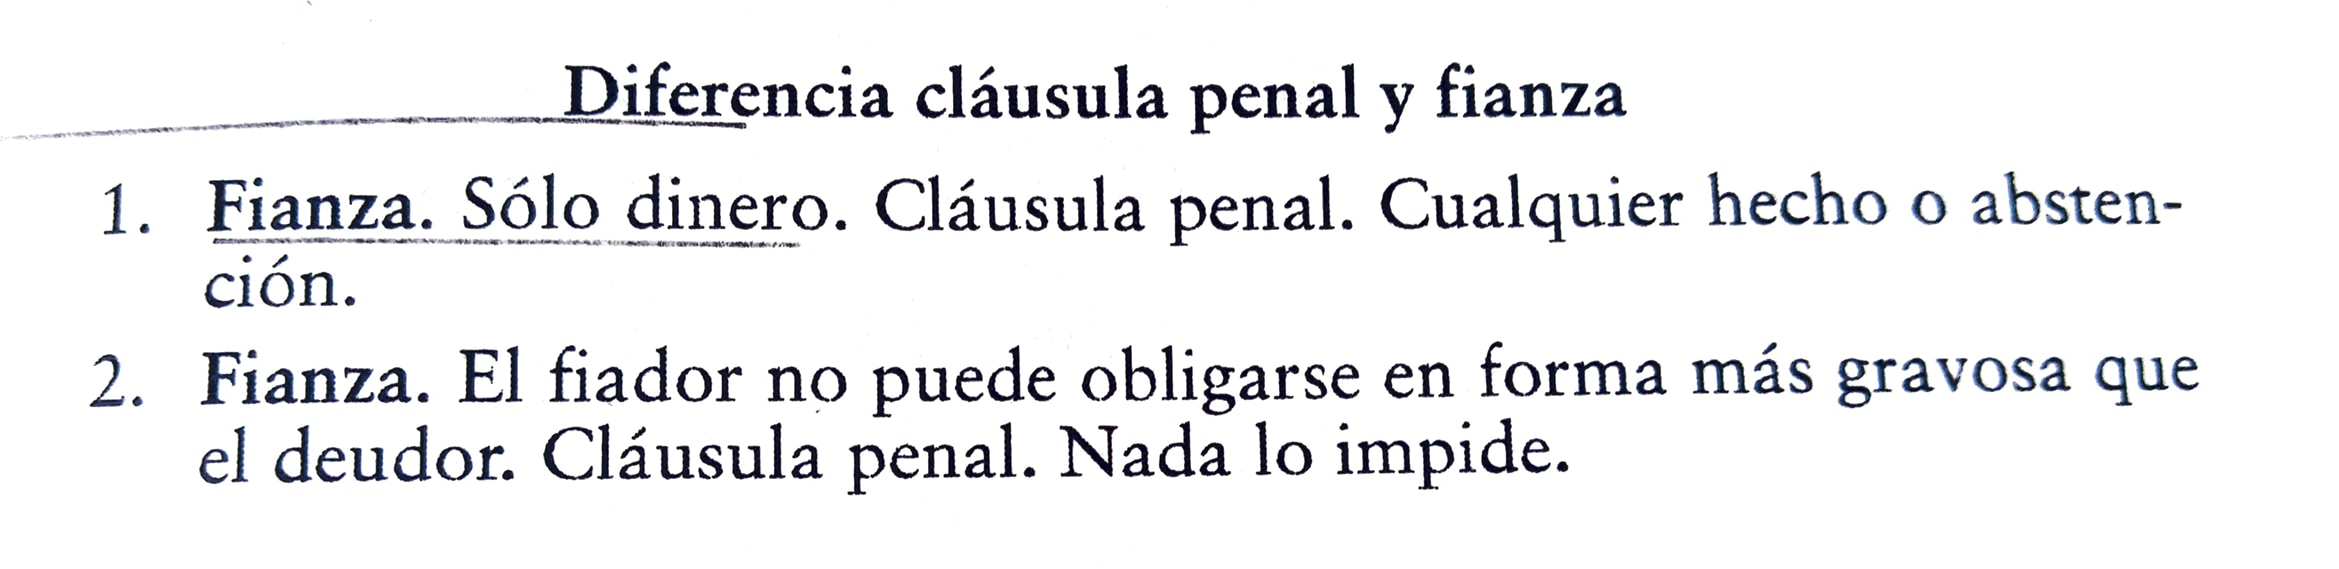
\includegraphics{dif.jpeg}
      \caption{Alt text}
      \end{figure}

      \begin{itemize}
      \tightlist
      \item
        reducción de la pena

        \begin{enumerate}
        \def\labelenumi{\arabic{enumi}.}
        \tightlist
        \item
          cuando acreedor acepta un pago parcial
        \item
          cuando la pena es enorme (contratos conmutativos = si excede
          del duplo de la obligación; mutuo = si excede los intereses
          penales; demás casos entregado a la prudencia del juez)
        \end{enumerate}
      \end{itemize}
    \item
      \begin{enumerate}
      \def\labelenumi{\alph{enumi})}
      \setcounter{enumi}{2}
      \tightlist
      \item
        \textbf{Que se impute a dolo o culpa del deudor}
      \end{enumerate}

      \begin{itemize}
      \item
        grados de imputación:

        \begin{itemize}
        \tightlist
        \item
          Caso fortuito o fuerza mayor
        \item
          Culpa
        \item
          Dolo
        \end{itemize}
      \item
        caso fortuito o fuerza mayor

        es un imprevisto que no es posible resistir. Exime de
        responsabilidad al deudor respecto a su incumplimiento o
        retardo. Si es parcial lo exime respecto a esa parcialidad.

        requisitos:

        \begin{itemize}
        \tightlist
        \item
          debe ser \emph{ajeno}
        \item
          imprevisto al momento de la celebración
        \item
          irresistible o insuperable
        \item
          imposibilidad \emph{permanente}
        \end{itemize}

        efectos:

        \begin{itemize}
        \item
          deudor queda \emph{exento} de responsabilidad
        \item
          no responde del retardo
        \item
          si deudor no puede cumplir \emph{parte}, queda liberado de
          esta parte

          \begin{itemize}
          \tightlist
          \item
            no exime

            \begin{enumerate}
            \def\labelenumi{\arabic{enumi}.}
            \tightlist
            \item
              estipulación expresa de las partes
            \item
              caso fortuito por culpa del deudor
            \item
              caso fortuito durante la mora
            \item
              caso de hurto y robo
            \end{enumerate}
          \end{itemize}
        \item
          teoría de la imprevisión

          se trata de una eximente de responsabilidad basada en la
          ocurrencia de un acontecimiento en condiciones generales,
          imprevisible, ajeno a la voluntad de las partes trastorna
          gravemente el equilibrio de las prestaciones de un contrato de
          tracto sucesivo, haciéndolo excesivamente oneroso el
          cumplimiento
        \item
          teoría de los riesgos

          es la que determina quien sufre en definitiva la pérdida de la
          cosa debida en los contratos bilaterales cuando está pendiente
          el cumplimiento de una obligación de dar o entregar una
          especie o cuerpo cierto.

          RG = el riesgo del cuerpo cierto cuya entrega se debe es
          siempre del acreedor
        \end{itemize}
      \item
        imputación por dolo o culpa

        \begin{itemize}
        \item
          dolo

          consiste en la intención positiva de inferir injuria a la
          persona o propiedad de otro

          Triple ámbito de aplicación del dolo:

          \begin{itemize}
          \item
            Como vicio del consentimiento
          \item
            Como agravante de la responsabilidad contractual
          \item
            Como elemento constitutivo de la responsabilidad
            extracontractual
          \item
            efectos

            \begin{enumerate}
            \def\labelenumi{\arabic{enumi}.}
            \tightlist
            \item
              da lugar a la indemnización de perjuicios
            \item
              agrava la responsabilidad del deudor
            \item
              origina responsabilidad solidaria
            \item
              puede ser renunciada (no anticipadamente)
            \end{enumerate}
          \item
            características

            \begin{itemize}
            \tightlist
            \item
              no se presumen, salvo:

              \begin{itemize}
              \tightlist
              \item
                albacea (art. 1301)
              \item
                ocultación del testamento (art. 968 n°5)
              \item
                la apuesta (art. 2261)
              \item
                medidas prejudiciales (art. 280 CPC)
              \end{itemize}
            \item
              no se puede condonar anticipada
            \item
              equivale a culpa grave
            \item
              el dolo no se gradúa
            \item
              las partes pueden atenuar la responsabilid del dolo
            \item
              se presume de hechos
            \end{itemize}
          \end{itemize}
        \item
          culpa

          es la falta de diligencia en el cumplimiento de una obligación
          o en la ejecución de un hecho cualquiera

          \begin{itemize}
          \tightlist
          \item
            clasificación

            \begin{itemize}
            \item
              culpa incontraendo

              la que proviene de un pacto tácito al celebrar un contrato
              que no se perfeccionó o resulto ineficaz
            \item
              culpa contractual

              es la que incide en el cumplimiento de obligaciones
              contractuales, cuasi contractuales y legales
            \item
              culpa extracontractual

              falta de cuidado general que hay que emplear en la
              ejecución de hechos para evitar perjuicios a terceros
            \end{itemize}
          \item
            clases (o graduaciones)

            \begin{itemize}
            \item
              culpa grave

              es la que consiste en no manejar los negocios ajenos con
              aquel cuidado que aún las personas negligentes y de poca
              prudencia suelen emplear en sus negocios propios

              \begin{itemize}
              \tightlist
              \item
                responden

                \begin{enumerate}
                \def\labelenumi{\arabic{enumi}.}
                \tightlist
                \item
                  todo deudor, aun cuando el acreedor esté en mora
                \item
                  deudor en contratos que solo son útiles al acreedor
                \item
                  cuando así lo han estipulado expresamente las partes
                \end{enumerate}
              \end{itemize}
            \item
              culpa leve RG

              es la falta de aquella diligencia y cuidado que los
              hombres emplean ordinariamente en sus negocios propios.

              \begin{itemize}
              \tightlist
              \item
                responden

                \begin{enumerate}
                \def\labelenumi{\arabic{enumi}.}
                \tightlist
                \item
                  deudor en los contratos onerosos
                \item
                  los que administran bienes ajenos
                \item
                  el que tiene el uso y goce de una cosa
                \item
                  cuando la ley le impone
                \item
                  cuando se ha estipulado expresamente
                \end{enumerate}
              \end{itemize}
            \item
              culpa levísima

              es la falta de aquella esmerada diligencia que un hombre
              juicioso emplea en la administración de sus negocios
              importantes. Responde de esta culpa el deudor en aquellos
              contratos en que el es el único beneficiario
            \end{itemize}
          \end{itemize}
        \end{itemize}
      \end{itemize}
    \item
      \begin{enumerate}
      \def\labelenumi{\alph{enumi})}
      \setcounter{enumi}{3}
      \item
        \textbf{Que el deudor esté constituido en mora}

        La mora es el retardo culpable en el cumplimiento de una
        obligación, más allá del plazo fijado para su ejecución o que
        persiste después del requerimiento
      \end{enumerate}

      \begin{itemize}
      \item
        requisitos

        \begin{enumerate}
        \def\labelenumi{\arabic{enumi}.}
        \tightlist
        \item
          retardo en el cumplimiento
        \item
          retardo culpable (dolo o culpa)
        \item
          interpelación

          \begin{itemize}
          \tightlist
          \item
            contractual

            \begin{itemize}
            \tightlist
            \item
              expresa = cuando no ha cumplido dentro del término
              estipulado (salvo que la ley lo establezca como en el caso
              de la cosa arrendada)
            \item
              tácita = cuando la cosa no ha podido ser dada o ejecutada
              sino dentro de cierto lapso
            \end{itemize}
          \item
            extracontractual

            \begin{itemize}
            \tightlist
            \item
              cuando ha sido reconvenido judicialmente, desde la
              notificación
            \end{itemize}
          \end{itemize}
        \item
          que el acreedor haya cumplido, por su parte, la obligación o
          manifieste estar llano a cumplirla
        \end{enumerate}

        \begin{itemize}
        \tightlist
        \item
          Efectos de la mora:

          \begin{itemize}
          \tightlist
          \item
            Impone al deudor la obligación de indemnizar perjuicios
          \item
            Hace el deudor responsable del caso fortuito que sobreviene
            durante la mora
          \item
            Pone a cargo del deudor el riesgo de la especie o cuerpo
            cierto que se debe
          \end{itemize}
        \item
          Efectos de la mora del \textbf{acreedor}:

          \begin{itemize}
          \tightlist
          \item
            Atenúa la responsabilidad del deudor, sólo responde de culpa
            lata o dolo
          \item
            El acreedor debe indemnizar los perjuicios
          \item
            No exonera al deudor. Debe pagar por consignación
          \end{itemize}
        \end{itemize}
      \item
        Excepción: la mora purga la mora

        en los contratos bilaterales, ninguno de los contratantes está
        en mora dejando de cumplir lo pactado, mientras el otro no lo
        cumple por su parte, o se allana a cumplirlo en la forma y
        tiempo debido.
      \item
        efectos

        \begin{enumerate}
        \def\labelenumi{\arabic{enumi}.}
        \tightlist
        \item
          impone al deudor la obligación de indemnizar perjuicios
        \item
          hace al deudor responsable del caso fortuito que sobreviene
          durante la mora.
        \item
          pone a cargo del deudor el riesgo de la especie o cuerpo
          cierto que se debe.
        \end{enumerate}
      \end{itemize}
    \item
      inexistencia de una cláusula de irresponsabilidad que exima de
      indemnización de perjuicios en caso de incumplimiento.
    \end{itemize}
  \item
    \begin{enumerate}
    \def\labelenumi{\arabic{enumi}.}
    \setcounter{enumi}{2}
    \tightlist
    \item
      Derechos auxiliares del acreedores
    \end{enumerate}

    \begin{itemize}
    \item
      \begin{enumerate}
      \def\labelenumi{\alph{enumi})}
      \tightlist
      \item
        medidas conservativas
      \end{enumerate}

      \begin{itemize}
      \tightlist
      \item
        guarda y aposición de sellos
      \item
        derechos del acreedor condicional
      \item
        derecho legal de retención del arrendatario, vendedor,
        mandatario, depositario, comodatario
      \item
        la herencia yacente
      \item
        medidas precautorias
      \item
        fideicomisario, asignatario y el acreedor condición
      \end{itemize}
    \item
      \begin{enumerate}
      \def\labelenumi{\alph{enumi})}
      \setcounter{enumi}{1}
      \tightlist
      \item
        acción subrogatoria u oblicua
      \end{enumerate}

      consiste en el ejercicio por los acreedores de acciones y derechos
      que competen al deudor para incorporar al patrimonio de éste,
      bienes en que hacer afectivos sus créditos

      \begin{itemize}
      \tightlist
      \item
        requisitos

        \begin{enumerate}
        \def\labelenumi{\arabic{enumi}.}
        \tightlist
        \item
          disposición legal que la conceda, deudor insolvente
        \item
          crédito cierto y exigible
        \item
          deudor se rehuse o descuide el ejercicio de sus acciones
        \item
          que la negativa o desidia perjudique al acreedor
        \end{enumerate}
      \item
        casos que procede

        \begin{enumerate}
        \def\labelenumi{\arabic{enumi}.}
        \tightlist
        \item
          derechos reales de usufructo, prenda e hipoteca (excp. los
          personalísimos)
        \item
          derecho legal de retención
        \item
          contrato de arrendamiento
        \item
          en acciones contra aquellos que por hecho o culpa suya pereció
          la cosa
        \item
          respecto a la repudiación de una herencia o legado
        \end{enumerate}
      \item
        efectos

        \begin{enumerate}
        \def\labelenumi{\arabic{enumi}.}
        \tightlist
        \item
          demandado puede oponer las excepciones que tenía contra el
          deudor
        \item
          sentencia produce cosa juzgada respecto del deudor
        \item
          los bienes que ingresan benefician a todos los acreedores
        \end{enumerate}
      \end{itemize}
    \item
      \begin{enumerate}
      \def\labelenumi{\alph{enumi})}
      \setcounter{enumi}{2}
      \tightlist
      \item
        acción revocatoria o pauliana
      \end{enumerate}

      es la que tiene los acreedores para obtener que se deje sin efecto
      las enajenaciones hechas por el deudor en fraude o con perjuicio a
      sus derechos

      \begin{itemize}
      \tightlist
      \item
        requisitos

        \begin{enumerate}
        \def\labelenumi{\arabic{enumi}.}
        \tightlist
        \item
          perjuicio de los acreedores
        \item
          fraude o mala fe (actos gratuitos = solo del deudor, onerosos
          = del deudor y del tercero con quien contrata)
        \end{enumerate}
      \item
        efectos

        \begin{enumerate}
        \def\labelenumi{\arabic{enumi}.}
        \tightlist
        \item
          se reintegra la cosa
        \item
          sólo aprovecha los acreedores, no el deudor
        \item
          sólo a los acreedores que han sido parte
        \item
          sólo hasta el monto debido
        \item
          los terceros pueden enervar, pagando
        \item
          prescribe en un año
        \end{enumerate}
      \end{itemize}
    \item
      \begin{enumerate}
      \def\labelenumi{\alph{enumi})}
      \setcounter{enumi}{3}
      \tightlist
      \item
        beneficio de separación
      \end{enumerate}

      consiste en un derecho auxiliar de los acreedores hereditarios y
      testamentarios para pedir que no se confundan los bienes del
      difunto con los bienes del heredero. Con esto, tendrán derecho a
      que de los bienes del difunto se les cumplan las obligaciones
      hereditarias o testamentarias con preferencia a las deudas propias
      del heredero
    \end{itemize}
  \end{itemize}
\item
  Modos de extinguir las obligaciones

  \begin{itemize}
  \item
    la resciliación o mutuo disenso

    es una convención entre acreedor y deudor, por la cual ambos,
    teniendo capacidad de disposición, consienten en extinguir la
    obligación, dejando sin efecto el contrato

    No procede respecto: mandato, arrendamiento
  \item
    el pago o solución

    es la prestación de lo que se debe y de todo lo que se debe. Se
    trata de un acto jurídico bilateral.

    \begin{itemize}
    \item
      quién puede pagar

      \begin{itemize}
      \tightlist
      \item
        el deudor
      \item
        una persona interesada
      \item
        un extraño (no interesado)
      \item
        requisitos respecto a la obligación de dar

        \begin{enumerate}
        \def\labelenumi{\arabic{enumi}.}
        \tightlist
        \item
          que sea dueño de la cosa o
        \item
          que tenga capacidad para enajenar
        \item
          solemnidades legales
        \end{enumerate}
      \end{itemize}
    \item
      a quién se debe realizar el pago?

      \begin{itemize}
      \tightlist
      \item
        al acreedor, herederos, legatarios o cesionarios
      \item
        al representante del acreedor
      \item
        al poseedor del crédito
      \end{itemize}
    \item
      forma de pago

      debe ser de conformidad al tenor de la obligación, de forma
      íntegra, y específico, con la misma cosa debida (especie o cuerpo
      cierto).

      \begin{itemize}
      \tightlist
      \item
        excepciones

        \begin{enumerate}
        \def\labelenumi{\arabic{enumi}.}
        \tightlist
        \item
          obligaciones modales
        \item
          obligaciones facultativas
        \item
          dación en pago
        \item
          total, salvo caso de convención en contrario
        \item
          la parte no disputada
        \item
          en la compensación
        \end{enumerate}
      \end{itemize}
    \item
      lugar del pago

      \begin{itemize}
      \tightlist
      \item
        lugar designado por la convención
      \item
        especie o cuerpo cierto, en lugar en que exista al constituirse
        la obligación
      \item
        si es otra cosa, en el domicilio del deudor al constituirse la
        obligación
      \end{itemize}
    \item
      qué se debe pagar?

      \begin{itemize}
      \item
        \textbf{oº de especie o cuerpo cierto}

        la cosa debe entregarse en el estado en que se encuentra

        \begin{itemize}
        \tightlist
        \item
          excepciones

          \begin{itemize}
          \tightlist
          \item
            rescisión del contrato y la indemnización de perjuicios

            \begin{enumerate}
            \def\labelenumi{\arabic{enumi}.}
            \tightlist
            \item
              si la cosa se deterioró por culpa del deudor
            \item
              por persona por la cual él es responsable,
            \item
              que hayan ocurrido después que el deudor estuviere en mora
            \item
              que no provengan de caso fortuito que hubiese ocurrido
              igualmente en manos del acreedor
            \end{enumerate}
          \item
            solamente indemnización de perjuicios

            \begin{enumerate}
            \def\labelenumi{\arabic{enumi}.}
            \tightlist
            \item
              si el acreedor prefiere llevarse la especie
            \item
              deterioro no pareciere de importancia
            \end{enumerate}
          \item
            pago válido en el estado que se encuentre pero el acreedor
            puede exigir que se le ceda la acción que tenga su deudor
            contra tercero

            \begin{enumerate}
            \def\labelenumi{\arabic{enumi}.}
            \tightlist
            \item
              deterioro ha sobrevenido antes de que el deudor se
              constituyera en mora pero por culpa de un tercero por la
              cual no es responsable
            \end{enumerate}
          \end{itemize}
        \item
          no responde de la pérdida

          \begin{enumerate}
          \def\labelenumi{\arabic{enumi}.}
          \tightlist
          \item
            por caso fortuito
          \item
            estando en mora, pero de haberse cumplido oportunamente la
            obligación la cosa se hubiere deteriorado igualmente en
            poder del acreedor
          \item
            por hechos de terceros que no responde el deudor
          \item
            destrucción de la cosa ofrecida al acreedor
          \end{enumerate}
        \end{itemize}
      \item
        \textbf{oº de genero}

        \begin{enumerate}
        \def\labelenumi{\arabic{enumi}.}
        \tightlist
        \item
          acreedor no puede pedir un individuo determinado
        \item
          deudor puede pagar con un individuo indeterminado de un género
          determinado, de una calidad de a lo menos mediana (con excp.
          mutuo: debe ser del mismo genero y calidad)
        \end{enumerate}
      \item
        \textbf{oº de dinero}

        \begin{enumerate}
        \def\labelenumi{\arabic{enumi}.}
        \tightlist
        \item
          sólo suma numérica
        \item
          puede ser reajustable
        \item
          se puede pactar en moneda extranjera o valor oro
        \end{enumerate}
      \end{itemize}
    \item
      imputación del pago

      es su aplicación a determinada obligación cuando entre acreedor y
      deudor existen varias obligaciones de la misma naturaleza, como
      intereses y el pago que efectúa no es suficiente para satisfacer
      su totalidad

      \begin{itemize}
      \tightlist
      \item
        requisitos

        \begin{enumerate}
        \def\labelenumi{\arabic{enumi}.}
        \tightlist
        \item
          varias obligaciones o una que produzca intereses
        \item
          entre los mismos acreedores y deudores
        \item
          que sean de la misma naturaleza
        \item
          que el pago sea insuficiente para todas
        \end{enumerate}
      \end{itemize}
    \item
      prueba

      \begin{enumerate}
      \def\labelenumi{\arabic{enumi}.}
      \tightlist
      \item
        incumbe al deudor
      \item
        limitación prueba testimonial si es superior a 2 UTM
      \item
        por recibo del pago, el cual tiene dº a exigir según C. de Com.
      \end{enumerate}
    \item
      modalidades del pago

      \begin{itemize}
      \item
        pago por consignación

        es el depósito de la cosa que se debe, con las formalidades
        necesarias, en manos de un tercero, hecho en virtud de
        repugnancia o no comparecencia del acreedor a recibirla, o de la
        incertidumbre acerca de su persona.

        \begin{itemize}
        \tightlist
        \item
          etapas

          \begin{itemize}
          \item
            oferta

            es el acto por el cual el deudor manifiesta su intención de
            cumplir la obligación
          \item
            consignación

            \begin{enumerate}
            \def\labelenumi{\arabic{enumi}.}
            \tightlist
            \item
              en la cuenta del TRB
            \item
              en la Tesorería comunal
            \item
              departamento agrícola del Banco Estado
            \item
              ferias, casas de martillo o almacenes de depósito del
              lugar en que debe hacerse el pago, según la naturaleza de
              la cosa
            \item
              en su defecto, al que nombrare el juez
            \end{enumerate}
          \item
            declaración de suficiencia del pago

            la realiza el juez y extingue la obligación.

            no la declarará cuando no comprenda la cosa debida o cuando
            se omitieron los requisitos de la oferta y consignación.
          \end{itemize}
        \end{itemize}
      \item
        pago con subrogación

        es una ficción legal por la cual el crédito que ha sido pagado
        con dineros proporcionados por un tercero, y que, por
        consiguiente se extingue respecto del acreedor, se reputa
        subsistir con todos sus accesorio, en provecho del tercero para
        asegurarle el reembolso de lo pagado.

        \begin{itemize}
        \item
          Requisitos:

          \begin{itemize}
          \tightlist
          \item
            pago de deuda ajena
          \item
            debe ser voluntario
          \item
            con fondos propios
          \item
            quien paga debe quedar en la misma situación jurídica que el
            acreedor
          \end{itemize}
        \item
          casos de subrogación legal (aún contra la voluntad del
          acreedor)

          \begin{enumerate}
          \def\labelenumi{\arabic{enumi}.}
          \tightlist
          \item
            del acreedor que paga a otro acreedor en razón de un
            privilegio o hipoteca
          \item
            del que habiendo comprado un inmueble es obligado a pagar a
            los acreedores hipotecarios
          \item
            del que paga una deuda a la que se halla obligado
            solidariamente o subsidiariamente
          \item
            del heredero beneficiario que paga las deudas de la herencia
          \item
            del que paga deuda ajena, consintiéndolo expresa o
            tácitamente con el deudor
          \item
            del que ha prestado dinero al deudor para el pago, constando
            en escritura pública
          \end{enumerate}
        \item
          subrogación convencional

          es aquella que se efectúa en virtud de una convención del
          acreedor y del tercero \textbf{no interesado} que le paga,
          subrogándole en todos los derechos y acciones que le
          corresponden
        \end{itemize}
      \item
        pago por cesión de bienes

        es el abandono voluntario que el deudor hace de todos sus bienes
        a su acreedor o acreedores cuando, a consecuencia de accidentes
        inevitables, no se halla en estado de pagar sus deudas.
      \item
        pago con beneficio de competencia

        es el que se concede a ciertos deudores para no ser obligados a
        pagar más de lo que buenamente puedan, dejándoseles en
        consecuencia lo indispensable para la modesta subsistencia,
        según clase y circunstancias, y con cargo de devolución, cuando
        mejoren de fortuna

        \begin{itemize}
        \tightlist
        \item
          ¿quienes pueden invocar este beneficio?

          \begin{enumerate}
          \def\labelenumi{\arabic{enumi}.}
          \tightlist
          \item
            ascendientes y descendientes
          \item
            cónyuge
          \item
            hermanos
          \item
            consocios
          \item
            donante, para cumplir la donación
          \item
            el que hizo cesión de bienes
          \end{enumerate}
        \end{itemize}
      \end{itemize}
    \end{itemize}
  \item
    dación en pago

    es una convención entre acreedor y deudor por la cual el deudor paga
    con una prestación diversa a la que se obliga.

    Efectos:

    \begin{itemize}
    \tightlist
    \item
      Si se considera novación = extingue el pago y no revive aunque la
      cosa sea evicta
    \item
      Si se la considera modalidad = revive la obligación si es evicta
    \end{itemize}
  \item
    novación

    es la sustitución de una nueva obligación a otra anterior, la cual
    queda extinguida. Es convención y contrato de carácter extintivo y
    sustitutivo.
  \item
    remisión

    Consiste en una convención en la cual el acreedor renuncia total o
    parcialmente de su crédito
  \item
    compensación

    consiste en un modo de extinguir las obligaciones en que ambas
    partes comparten la calidad de acreedor y deudor, extinguiéndose
    ambas obligaciones hasta la concurrencia de la de menor valor,
    reuniéndose los demás requisitos legales.

    Requisitos:

    \begin{itemize}
    \tightlist
    \item
      partes recíprocamente acreedoras y deudoras
    \item
      obligaciones de igual naturaleza
    \item
      obligaciones deben ser exigibles
    \item
      liquidez de ambas deudas
    \end{itemize}

    Hechos que impiden la compensación:

    \begin{itemize}
    \tightlist
    \item
      que la obligación sea natural
    \item
      condición suspensiva pendiente
    \item
      plazo no vencido
    \end{itemize}

    Obligaciones no compensables:

    \begin{itemize}
    \tightlist
    \item
      demanda de restitución de un despojo
    \item
      demanda de indemnización por violencia o fraude
    \item
      demanda de alimentos
    \end{itemize}
  \item
    confusión

    modo de extinguir las obligaciones que, opera de pleno derecho y que
    se produce cuando en una misma persona concurren las calidades de
    acreedor y deudor
  \item
    pérdida de la cosa que se debe

    se produce cuando la cosa se destruye, desaparece, ignorándose si
    existe y cuando deja de estar en el comercio. Puede producir o la
    responsabilidad del deudor o liberarlo de ella.

    \begin{itemize}
    \tightlist
    \item
      lo libera de responsabilidad

      \begin{enumerate}
      \def\labelenumi{\arabic{enumi}.}
      \tightlist
      \item
        cuando es producida por caso fortuito o fuerza mayor
      \item
        cuando la cosa se destruye estando en poder del deudor, después
        de haber sido ofrecida al acreedor y durante el retardo de éste
        en recibirla (mora del acreedor)
      \end{enumerate}
    \item
      produce la responsabilidad del deudor

      \begin{enumerate}
      \def\labelenumi{\arabic{enumi}.}
      \tightlist
      \item
        hecho o culpa suyo
      \item
        se produce por fuerza mayor o caso fortuito durante mora de el
      \item
        cuando el deudor ha tomado para sí la responsabilidad
      \item
        pérdida de la cosa por caso fortuito o fuerza mayor, en manos de
        quién la ha hurtado o robado (aun cuando se hubiera producido
        igualmente en manos del acreedor)
      \end{enumerate}
    \end{itemize}
  \item
    prescripción

    es un modo de \emph{extinguir} las acciones y derechos ajenos por no
    haberse ejercido dichas acciones y derechos durante cierto lapso de
    tiempo y concurriendo los demás requisitos legales, es decir, no
    extingue la obligación civil propiamente tal sino que simplemente la
    transforma en natural, extinguiendo la acción para exigir su
    cumplimiento.

    \begin{itemize}
    \tightlist
    \item
      Requisitos:

      \begin{itemize}
      \item
        \begin{enumerate}
        \def\labelenumi{\Alph{enumi})}
        \tightlist
        \item
          Acción debe ser prescriptible

          \begin{itemize}
          \tightlist
          \item
            son imprescriptibles

            \begin{enumerate}
            \def\labelenumii{\arabic{enumii}.}
            \tightlist
            \item
              la acción de reclamación de estado civil
            \item
              acción para pedir la destrucción de una obra nueva que
              corrompa el aire o la haga conocidamente dañoso
            \item
              la acción de divorcio, separación judicial y nulidad del
              matrimonio
            \item
              acción para pedir la partición
            \end{enumerate}
          \end{itemize}
        \end{enumerate}
      \item
        \begin{enumerate}
        \def\labelenumi{\Alph{enumi})}
        \setcounter{enumi}{1}
        \tightlist
        \item
          Debe ser alegada
        \end{enumerate}

        \begin{itemize}
        \tightlist
        \item
          Salvo: acción ejecutiva, en materia penal
        \end{itemize}
      \item
        \begin{enumerate}
        \def\labelenumi{\Alph{enumi})}
        \setcounter{enumi}{2}
        \tightlist
        \item
          Que no se haya interrumpido
        \end{enumerate}

        \begin{itemize}
        \item
          natural = por el hecho de reconocer el deudor la obligación,
          expresamente o de forma tácita
        \item
          civil = dda judicial notificada

          \begin{itemize}
          \tightlist
          \item
            Efectos de la interrupción:

            \begin{itemize}
            \tightlist
            \item
              detiene el curso de la prescripción
            \item
              hace perder todo el tiempo trascurrido
            \item
              son relativos, salvo solidaridad o indivisibilidad
            \end{itemize}
          \end{itemize}
        \end{itemize}
      \item
        \begin{enumerate}
        \def\labelenumi{\Alph{enumi})}
        \setcounter{enumi}{3}
        \tightlist
        \item
          Que no esté suspendida
        \end{enumerate}

        se suspende a favor de:

        \begin{itemize}
        \tightlist
        \item
          los menores
        \item
          dementes
        \item
          sordos
        \item
          sordomudos
        \item
          potestad paterna, tutela o curatela
        \item
          mujer casada en soc. conyugal
        \item
          siempre entre cónyuges
        \end{itemize}
      \item
        \begin{enumerate}
        \def\labelenumi{\Alph{enumi})}
        \setcounter{enumi}{4}
        \tightlist
        \item
          Transcurso del tiempo
        \end{enumerate}

        \begin{itemize}
        \tightlist
        \item
          se cuenta, por rg., desde que se hizo exigible
        \item
          el plazo por rg. es legal
        \item
          forma de contar establecida por el legislador art. 48 y ss.
        \end{itemize}
      \end{itemize}
    \end{itemize}
  \item
    \begin{enumerate}
    \def\labelenumi{\Alph{enumi})}
    \tightlist
    \item
      Prescripciones de largo tiempo

      \begin{itemize}
      \item
        acciones de obligaciones

        \begin{enumerate}
        \def\labelenumii{\arabic{enumii}.}
        \tightlist
        \item
          ejecutivas = 3 años
        \item
          ordinarias = 5 años
        \end{enumerate}
      \item
        acciones de obligaciones accesorias

        junto con la obligación principal 2516
      \item
        acciones propietarias

        \begin{itemize}
        \tightlist
        \item
          toda acción por la que se reclama un derecho se extingue por
          la prescripción adquisitiva de ese mismo derecho.
          Reivindicatoria: 2 y 5, 10 años (PAE)
        \item
          petición de herencia: 5 y 10 años (dependiendo si es heredero
          putativo)
        \item
          servidumbre: 3 años
        \end{itemize}
      \end{itemize}
    \end{enumerate}
  \item
    \begin{enumerate}
    \def\labelenumi{\Alph{enumi})}
    \setcounter{enumi}{1}
    \tightlist
    \item
      Prescripciones de corto tiempo
    \end{enumerate}

    \begin{itemize}
    \tightlist
    \item
      presuntivas de pago

      \begin{enumerate}
      \def\labelenumi{\arabic{enumi}.}
      \tightlist
      \item
        honorario de profesionales liberales: 2 años
      \item
        mercaderes, artesanos, servicios accidentales: 1 años
      \item
        impuestos: 3 años. 6 sujetos a declaración
      \end{enumerate}
    \item
      especiales

      \begin{enumerate}
      \def\labelenumi{\arabic{enumi}.}
      \tightlist
      \item
        despojo violento, redhibitoria muebles: 6 meses
      \item
        posesorias rebaja del precio: 1 año
      \item
        reforma de testamento, pacto de retroventa, responsabilidad
        extracontractual: 4 años
      \end{enumerate}
    \end{itemize}
  \item
    caducidad

    es una sanción legal que consiste en la extinción de un derecho por
    no haberse ejercido o cumplido una formalidad legal dentro del plazo
    fatal que la misma ley establece
  \end{itemize}
\end{itemize}

\hypertarget{fuentes-de-las-obligaciones}{%
\section{6. Fuentes de las
Obligaciones}\label{fuentes-de-las-obligaciones}}

\begin{itemize}
\tightlist
\item
  conceptos preliminares

  \begin{itemize}
  \item
    convención

    acto jurídico bilateral que tiene por finalidad crear, modificar o
    extinguir derechos y obligaciones
  \item
    contrato

    es un tipo de convención, es decir, un acto jurídico bilateral que
    tiene por finalidad crear derechos y obligaciones correlativas, en
    la cual una o ambas partes se obligan con la otra a satisfacer una
    necesidad jurídica que consiste en la realización de una prestación,
    la cual puede consistir en un dar, hacer o no hacer
  \end{itemize}
\end{itemize}

\hypertarget{contratos-en-general}{%
\subsection{6.1. Contratos en General}\label{contratos-en-general}}

\begin{itemize}
\item
  clasificación

  \begin{itemize}
  \tightlist
  \item
    unilaterales y bilaterales

    \begin{enumerate}
    \def\labelenumi{\arabic{enumi}.}
    \tightlist
    \item
      unilateral = una de las partes se obliga para con otra que no
      contrae obligación alguna. Mutuo, comodato, prenda, depósito
      (contratos reales)
    \item
      bilaterales = las partes contratantes se obligan recíprocamente.
      Compraventa, arrendamiento, transacción
    \end{enumerate}

    \begin{itemize}
    \tightlist
    \item
      importancia

      \begin{itemize}
      \tightlist
      \item
        \textbf{CRT}
      \item
        \textbf{teoría de los riesgos}
      \item
        \textbf{la mora purga la mora}
      \end{itemize}
    \end{itemize}
  \item
    gratuitos y onerosos

    \begin{enumerate}
    \def\labelenumi{\arabic{enumi}.}
    \tightlist
    \item
      gratuitos = sólo tiene por objeto la utilidad de una de las
      partes, sufriendo la otra el gravamen. Comodato, donación,
      depósito
    \item
      oneroso = tiene por objeto la utilidad de ambos contratantes,
      gravándose cada uno en beneficio del otro. Permuta, compraventa,
      mutuo con interés
    \end{enumerate}

    \begin{itemize}
    \tightlist
    \item
      importancia

      \begin{itemize}
      \tightlist
      \item
        \textbf{acción pauliana}
      \item
        \textbf{determinar grado de culpa}
      \item
        \textbf{error en la persona}
      \item
        \textbf{saneamiento de la evicción}
      \end{itemize}
    \end{itemize}
  \item
    conmutativos y aleatorios

    \begin{enumerate}
    \def\labelenumi{\arabic{enumi}.}
    \tightlist
    \item
      conmutativos = cada una de las partes se obliga a dar o hacer una
      cosa que se mira como equivalente a lo que la otra parte debe dar
      o hacer a su vez (se miran como equivalentes el sacrificio y el
      provecho)
    \item
      aleatorios = cuando el equivalente consiste en una contingencia
      incierta de ganancia o pérdida
    \end{enumerate}
  \item
    principales, accesorios y dependientes

    \begin{enumerate}
    \def\labelenumi{\arabic{enumi}.}
    \tightlist
    \item
      principales = aquellos que subsisten por sí mismos, sin necesidad
      de otra convención
    \item
      accesorios = cuando tienen por objeto asegurar el cumplimiento de
      una obligación principal, de manera que no puedan subsistir sin
      ella
    \item
      dependientes = no aseguran el cumplimiento. Capitulaciones
      matrimoniales, están subordinados en cuanto a sus efectos a otro
      contrato
    \end{enumerate}
  \item
    nominados e innominados

    \begin{enumerate}
    \def\labelenumi{\arabic{enumi}.}
    \tightlist
    \item
      nominados = tienen un nombre y una reglamentación legal
    \item
      Innominados = son creados por las partes
    \end{enumerate}
  \item
    consensuales, reales y solemnes

    \begin{enumerate}
    \def\labelenumi{\arabic{enumi}.}
    \tightlist
    \item
      consensuales = se perfeccionan por el solo consentimiento
    \item
      reales = se perfeccionan por la entrega o tradición de la cosa.
      Comodato, depósito, mutuo
    \item
      solemnes = está sujeto a ciertas formalidades, sin las cuales no
      producen ningún efecto civil, este carácter es dado por la ley.
      Instrumento público o privado, escrituración, presencia de un
      funcionario
    \end{enumerate}
  \item
    de ejecución instantánea y de tracto sucesivo

    \begin{enumerate}
    \def\labelenumi{\arabic{enumi}.}
    \tightlist
    \item
      ejecución instantánea = la obligación por su naturaleza solo puede
      cumplirse en un solo acto
    \item
      tracto sucesivo = la obligación por su naturaleza debe ser
      cumplida sucesivamente en el tiempo
    \end{enumerate}
  \item
    de libre discusión y adhesión

    \begin{enumerate}
    \def\labelenumi{\arabic{enumi}.}
    \tightlist
    \item
      libre discusión = ambas partes fijan las condiciones
    \item
      adhesión = una de las partes fija las condiciones y la otra se
      limita a prestar su aprobación
    \end{enumerate}
  \item
    individuales y colectivos

    \begin{enumerate}
    \def\labelenumi{\arabic{enumi}.}
    \tightlist
    \item
      individuales = requieren el consentimiento unánime de todas las
      partes
    \item
      colectivos = aquellos que obligan no solo a los que concurrieron a
      él, sino a los que se agregan al mismo grupo
    \end{enumerate}
  \end{itemize}
\item
  autocontrato

  es el que celebra una persona consigo misma y en el cual actúa a la
  vez por sí y como representante de otro y como representante de ambas.
\item
  efectos de los contratos

  \begin{itemize}
  \item
    entre las partes

    \begin{enumerate}
    \def\labelenumi{\arabic{enumi}.}
    \tightlist
    \item
      es una ley para los contratantes y no puede ser invalidado sino
      por su mutuo disenso o causales legales art. 1545
    \item
      buena fe y obligan a todas las cosas que emanan de su naturaleza o
      que por la ley o costumbre pertenezcan a el art. 1546
    \end{enumerate}
  \item
    respecto a terceros

    \begin{itemize}
    \item
      absolutos

      efecto relativo de los contratos, nunca van a estar en relación
      con las partes.

      \begin{itemize}
      \tightlist
      \item
        excepción

        \begin{itemize}
        \item
          actos de familia
        \item
          contratos colectivos
        \item
          estipulación a favor de otro

          es un contrato en que una de las partes (estipulante),
          conviene con la otra (promitente), que ésta realizará una
          determinada prestación en favor de un 3º extraño a la
          convención (beneficiario). p.~ej. contrato de seguro
        \item
          promesa por otro

          es una convención en que uno de los contratantes se compromete
          a dar, hacer o no hacer alguna cosa por una tercera persona de
          quien no es legítimo representante art. 1450
        \end{itemize}
      \end{itemize}
    \item
      relativos

      entran en la relación con las partes con posterioridad. ej. los
      herederos, los legatarios

      \begin{itemize}
      \item
        sucesores a título universal

        representan al causante, identificándose con él

        \begin{itemize}
        \tightlist
        \item
          excepción

          \begin{itemize}
          \tightlist
          \item
            obligaciones intrasmisibles
          \item
            contratos intuito personae
          \item
            cuando se ha estipulado expresamente
          \end{itemize}
        \end{itemize}
      \item
        sucesores a título singular

        \begin{enumerate}
        \def\labelenumi{\arabic{enumi}.}
        \tightlist
        \item
          sucesor hace suyas las ventajas y soporta los gravámenes
          p.~ej. hipoteca
        \item
          deben ser anteriores a la adquisición
        \item
          deben referirse al bien adquirido
        \end{enumerate}
      \item
        acreedores

        \begin{enumerate}
        \def\labelenumi{\arabic{enumi}.}
        \tightlist
        \item
          caso de la acción pauliana o revocatoria
        \item
          impugnación por simulación
        \end{enumerate}
      \end{itemize}
    \end{itemize}
  \item
    teoría de la inoponibilidad

    es la ineficacia respecto de terceros de un derecho nacido como
    consecuencia de la celebración o de la declaración de nulidad de un
    acto

    \begin{itemize}
    \tightlist
    \item
      \textbf{por defecto de forma}

      \begin{itemize}
      \item
        por falta de \emph{publicidad}

        \begin{enumerate}
        \def\labelenumi{\arabic{enumi}.}
        \tightlist
        \item
          falta de inscripción de embargos o precautorias en inmuebles
        \item
          falta de inscripción de la sentencia que declara la
          prescripción adquisitiva de inmuebles
        \item
          falta de anotación marginal de la contraescritura
        \item
          falta de publicación e inscripción del decreto de interdicción
        \item
          en la cesión de derechos, no produce efecto alguno mientras no
          ha sido notificada por el cesionario al deudor o aceptado por
          éste
        \end{enumerate}
      \item
        por falta de \emph{fecha cierta}

        art. 1703 CC la fecha de instrumento privado no se cuenta
        respecto de terceros sino desde:

        \begin{itemize}
        \tightlist
        \item
          el fallecimiento de uno de los que han firmado
        \item
          el día en que ha sido copiado en un registro público
        \item
          que conste haberse presentado en juicio
        \item
          que haya tomado razón de él o le haya inventariado un
          funcionario competente, en carácter de tal
        \end{itemize}
      \end{itemize}
    \item
      \textbf{por defecto de fondo}

      \begin{itemize}
      \tightlist
      \item
        casos

        \begin{itemize}
        \item
          por fraude

          es el caso de la acción revocatoria o pauliana
        \item
          lesión de derechos adquiridos

          la rescisión del decreto de posesión efectiva
        \item
          lesión de asignaciones forzosas

          la acción de reforma de testamento
        \item
          por falta de concurrencia

          \begin{enumerate}
          \def\labelenumi{\arabic{enumi}.}
          \tightlist
          \item
            la venta de cosa ajena
          \item
            los límites del mandato
          \item
            inoponibilidad de la nulidad en los casos de sociedad y
            matrimonio
          \end{enumerate}
        \end{itemize}
      \end{itemize}
    \end{itemize}
  \end{itemize}
\item
  interpretación de los contratos

  \begin{enumerate}
  \def\labelenumi{\arabic{enumi}.}
  \tightlist
  \item
    se debe estar más a la intención de las partes que a lo literal del
    contrato
  \item
    los términos del contrato solo se aplican a la materia de que se
    trata, por más generales que sean
  \item
    se prefiere el sentido en que la cláusula no produzca efecto alguno
  \item
    se deberá preferir la interpretación que mejor cuadre con la
    naturaleza del contrato, a menos que se señale lo contrario. Las
    cláusulas de uso común se presumen.
  \item
    se interpretan las cláusulas dando el mejor sentido que convenga al
    contrato en su totalidad. Se pueden interpretar con otro contrato
    entre las mismas partes sobre la misma materia. También por la
    práctica que hacen las partes o una con aprobación de la otra
  \item
    en caso de que se ejemplifique con un caso, una obligación , no se
    entiende limitarla a los demás casos que naturalmente se extiende
  \item
    en el defecto de las normas anteriores se interpretan las cláusulas
    ambiguas a favor del deudor. Pero aquellas que se hayan dictadas por
    una de las partes se entenderán contra ella cuando se deba a una
    falta de explicación de su parte.
  \end{enumerate}
\end{itemize}

\hypertarget{contratos-en-particular}{%
\subsection{6.2. Contratos en
Particular}\label{contratos-en-particular}}

\begin{itemize}
\item
  promesa

  contrato en virtud del cual dos o más personas se obligan a celebrar
  un contrato futuro, concurriendo los requisitos legales

  Requisitos:

  \begin{itemize}
  \tightlist
  \item
    debe constar por escrito
  \item
    que el contrato prometido no sea de aquellos que las leyes declaran
    ineficaces
  \item
    debe contener un plazo o condición
  \item
    que se especifique de tal manera que solo falten la tradición o
    solemnidad que las leyes prescriben
  \end{itemize}
\item
  compraventa

  es un contrato en que una de las partes se obliga a dar una cosa y la
  otra a pagarla en dinero

  \begin{itemize}
  \tightlist
  \item
    Características:

    \begin{itemize}
    \tightlist
    \item
      principal
    \item
      nominado
    \item
      bilateral
    \item
      oneroso
    \item
      por rg. conmutativo
    \item
      por rg. consensual
    \item
      TTD
    \end{itemize}
  \item
    elementos

    \begin{itemize}
    \tightlist
    \item
      consentimiento libre y espontáneo (salvo la venta forzada)

      \begin{itemize}
      \tightlist
      \item
        Debe recaer sobre:

        \begin{itemize}
        \tightlist
        \item
          la cosa
        \item
          el precio
        \item
          la naturaleza del contrato
        \end{itemize}
      \end{itemize}
    \item
      la cosa (comerciable, determinada o determinable, real, no
      pertenecerle al comprador)
    \item
      precio fijado en dinero
    \item
      solemnidades en algunos casos
    \end{itemize}
  \item
    casos de compraventa solemnes

    \begin{itemize}
    \tightlist
    \item
      por escritura pública

      \begin{enumerate}
      \def\labelenumi{\arabic{enumi}.}
      \tightlist
      \item
        bienes raíces (salvo Serviu 14.171, caso de compraventa b. raíz
        por escritura privada)
      \item
        Servidumbre
      \item
        censos
      \item
        sucesión hereditaria
      \end{enumerate}
    \item
      con arras

      \begin{itemize}
      \tightlist
      \item
        como garantía de la celebración o ejecución del contrato
      \item
        como parte del precio o en señal de quedar convenidos
        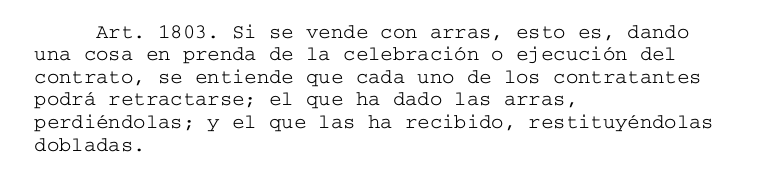
\includegraphics{arras.png}
      \end{itemize}
    \end{itemize}
  \item
    solemnidades

    \begin{itemize}
    \item
      legales

      \begin{itemize}
      \item
        ordinarias

        \begin{itemize}
        \tightlist
        \item
          escritura pública en el caso de los bienes raíces,
          servidumbres, censos, derecho de herencia (salvo 14.171
          escritura privada, firmada ante notario y protocolizada más
          tardar el día ss.)
        \item
          venta de inmuebles por adherencia y destinación
        \end{itemize}

        la tradición no es solemnidad en ningún caso. La solemnidad sólo
        es la escritura pública
      \item
        especiales

        son aquellas que están establecidas en atención a la calidad o
        estado de la persona que vende el bien, como es en el caso de
        los incapaces, venta b. raíces del hijo (escritura pública más
        autorización judicial) y el caso de autorización judicial más la
        subasta pública (venta de b. raíces del pupilo por parte de su
        curador)
      \end{itemize}
    \item
      voluntarias

      los que las partes establezcan, su omisión no produce la nulidad,
      solamente se tendrá como consensual
    \item
      venta forzada en juicio ejecutivo

      se consideran contrato de compraventa, juez actúa como
      representante legal del vendedor o deudor, y el precio se fija
      mediante la puja de los interesados (mejor postor)
    \end{itemize}
  \item
    efectos

    \begin{itemize}
    \tightlist
    \item
      obligaciones del vendedor

      \begin{itemize}
      \item
        \begin{enumerate}
        \def\labelenumi{\Alph{enumi})}
        \tightlist
        \item
          entregar la cosa
        \end{enumerate}

        \begin{itemize}
        \tightlist
        \item
          conferir al comprador la posesión legal y material de la cosa
        \item
          si la cosa consiste en especie o cuerpo cierto además tiene la
          obligación de conservar la cosa hasta su entrega (salvo que
          sea de ejecución instantánea)
        \item
          forma de entregar

          \begin{itemize}
          \tightlist
          \item
            muebles art. 684
          \item
            inmuebles art 686
          \end{itemize}
        \item
          momento de entrega

          \begin{itemize}
          \tightlist
          \item
            tan pronto quede perfecto
          \item
            una vez cumplido el plazo, modo o estipulación convenida
          \end{itemize}
        \item
          lugar de entrega

          \begin{itemize}
          \tightlist
          \item
            lugar convenido
          \item
            donde se encontraba la especie o cuerpo cierto
          \item
            en el domicilio del deudor
          \end{itemize}
        \item
          gastos de la entrega

          \begin{itemize}
          \tightlist
          \item
            vendedor = gastos para poner la cosa en disposición de
            entregarla
          \item
            comprador = trasporte después de efectuada la entrega
          \end{itemize}
        \end{itemize}
      \item
        \begin{enumerate}
        \def\labelenumi{\Alph{enumi})}
        \setcounter{enumi}{1}
        \tightlist
        \item
          saneamiento
        \end{enumerate}

        \begin{itemize}
        \item
          evicción

          se produce cuando el comprador es privado de todo o parte de
          la cosa por sentencia judicial \textbf{anterior} a la compra

          Consiste en que el vendedor tiene la obligación de defender al
          comprador contra terceros (obligación de amparo) que reclamen
          derechos sobre la cosa e indemnizarlo si la evicción se
          produce

          tiene dos etapas:

          \begin{itemize}
          \tightlist
          \item
            obligación de amparo = defender al comprador en juicio
          \item
            obligación de indemnización = si se produce la privación
            total o parcial
          \item
            total

            \begin{enumerate}
            \def\labelenumi{\arabic{enumi}.}
            \tightlist
            \item
              restitución del precio, aunque haya disminuido su valor,
              salvo que se deba a deterioros que se haya aprovechado el
              vendedor
            \item
              costal legales
            \item
              costal judiciales, salvo caso del comprador contumaz
              (vendedor citado se allana y comprador sigue adelante
              perdiendo juicio)
            \item
              pago de frutos, salvo caso del comprador contumaz
            \item
              aumento de valor de la cosa

              \begin{itemize}
              \tightlist
              \item
                causas naturales, transcurso del tiempo = si estaba en
                buena fe con tope de 1/4 parte del precio de la venta
              \item
                mejoras = si estaba en buena fe, necesarias y útiles que
                no hayan sido abonadas por el que obtuvo la evicción
              \end{itemize}
            \end{enumerate}
          \item
            parcial

            \begin{enumerate}
            \def\labelenumi{\arabic{enumi}.}
            \tightlist
            \item
              si la parte evicta es tal que no habría comprado sin ella
              tiene derecho a pedir la rescisión de la venta
            \item
              si la parte no es tal o no se desee pedir su rescisión,
              tiene derecho a pedir la evicción parcial (restitución del
              precio parcial)
            \item
              corresponde no solo al vendedor directo sino los
              antecesores a él en el dominio
            \end{enumerate}
          \end{itemize}
        \item
          vicios redhibitorios

          derecho que tiene el comprador para que se rescinda la venta o
          se rebaje proporcionalmente el precio por los vicios ocultos
          de la cosa vendida, raíz o mueble

          \begin{itemize}
          \tightlist
          \item
            efectos

            \begin{enumerate}
            \def\labelenumi{\arabic{enumi}.}
            \tightlist
            \item
              acción redhibitoria (acción resolutoria del contrato)
            \item
              quanti minoris o estimatoria, acción para pedir
              restitución proporcional del precio
            \end{enumerate}
          \item
            extinción

            \begin{itemize}
            \item
              renuncia

              Es un elemento de la naturaleza por lo que puede ser
              renunciado por su comprador, siempre que no haya estado en
              mala fe
            \item
              prescripción

              \begin{itemize}
              \tightlist
              \item
                acción redhibitoria

                \begin{itemize}
                \tightlist
                \item
                  6 meses muebles
                \item
                  1 ano inmuebles
                \end{itemize}
              \item
                quantis minoris

                \begin{itemize}
                \tightlist
                \item
                  1 muebles
                \item
                  18 inmuebles
                \item
                  en el caso de que la cosas sea enviada a un lugar
                  distante, se contara desde la entrega mas el termino
                  de emplazamiento
                \end{itemize}
              \end{itemize}
            \item
              ventas forzadas

              a menos que el vendedor no pudiendo o no debiendo
              desconocer los vicios no los hubiera declarado a petición
              del comprador
            \end{itemize}
          \end{itemize}
        \end{itemize}
      \end{itemize}
    \item
      obligaciones del comprador

      \begin{enumerate}
      \def\labelenumi{\arabic{enumi}.}
      \tightlist
      \item
        recibir la cosa
      \end{enumerate}

      \begin{itemize}
      \tightlist
      \item
        efectos de la mora del comprador en recibir la cosa:

        \begin{itemize}
        \tightlist
        \item
          abonar perjuicios
        \item
          vendedor solo responderá de dolo o culpa grave
        \end{itemize}
      \end{itemize}

      \begin{enumerate}
      \def\labelenumi{\arabic{enumi}.}
      \setcounter{enumi}{1}
      \tightlist
      \item
        pagar el precio
      \end{enumerate}
    \end{itemize}
  \item
    Pactos Accesorios:

    \begin{itemize}
    \tightlist
    \item
      Pacto comisorio
    \item
      Pacto de retroventa
    \item
      Pacto de retracto
    \item
      Otros pactos conforme a las rg.
    \end{itemize}
  \end{itemize}
\item
  permuta

  Es el contrato por el cual las partes se obligan mutuamente a dar una
  especie o cuerpo cierto por otro

  Por rg. se aplican las normas sobre la CV en lo que no sea contrario a
  su naturaleza
\item
  cesión de derechos

  Consiste en el traspaso de un derecho por parte de su titular a otra
  persona por un acto entre vivos

  \begin{itemize}
  \item
    cesión de créditos personales

    Puede ser clasificada como a) al portador, b) a la orden, y, c)
    nominativo. El CC regula esta ultima, las dos primaras se encuentran
    reguladas por el C de Com.

    Se perfecciona por la entrega del título, anotándose en el documento
    el traspaso del derecho en la escritura, nombre del cesionario y
    firma del cedente, puede consistir en una entrega real o simbólica.

    Respecto al deudor de dicho crédito debe ser notificado
    judicialmente o haber aceptado (expresa o tácitamente)
  \item
    cesión del derecho de herencia o legado

    Procede una vez que se encuentre abierta la sucesión (luego de la
    muerte del causante), que se traspase toda la herencia o una cuota
    de ella, que sea hecha por el heredero o un tercero, y que sea a
    título oneroso.
  \item
    cesión de derechos litigiosos

    Son aquellos derechos cuya existencia es discutida en juicio, evento
    incierto de la litis, solo le corresponde al demandante. Se efectúa
    apersonándose el cesionario al juicio, acompañando el título de la
    cesión
  \end{itemize}
\item
  Arrendamiento

  Es un contrato en que las partes se obligan recíprocamente, la una a
  conceder el goce de una cosa, o a ejecutar una obra o prestar un
  servicio, y la otra a pagar por este goce, obra o servicio un precio
  determinado

  Características:

  \begin{itemize}
  \tightlist
  \item
    nominado
  \item
    bilateral, oneroso y conmutativo
  \item
    mera tolerancia
  \item
    consensual
  \item
    acto de administración
  \item
    trato sucesivo
  \item
    principal
  \end{itemize}

  Obligaciones del arrendador:

  \begin{itemize}
  \tightlist
  \item
    entregar la cosa
  \item
    mantenerla en el estado de servir
  \item
    librar al arrendatario de toda turbación o embarazo en el goce la
    cosa
  \item
    que la cosa sirva para los fines que se tuvieron en vista al
    contratar
  \end{itemize}

  Obligaciones del arrendatario:

  \begin{itemize}
  \tightlist
  \item
    pagar el precio o renta
  \item
    usar la cosa según los términos del contrato
  \item
    cuidar la cosa como un buen padre de familia
  \item
    efectuar las reparaciones locativas
  \item
    restituir la cosa al término del arrendamiento
  \end{itemize}
\item
  El Contrato de Mandato

  Características:

  \begin{itemize}
  \item
    nominado
  \item
    principal
  \item
    generalmente consensual
  \item
    naturalmente oneroso
  \item
    bilateral
  \item
    es solemne
  \item
    mandatario obra por cuenta y riesgo del mandante
  \item
    el mandato es un ctto. de confianza

    La representación no es de la esencia de mandato. El encargo debe
    consistir en la ejecución de actos jurídicos.
  \end{itemize}

  Obligaciones del mandatario:

  \begin{itemize}
  \tightlist
  \item
    ejecutar el mandato
  \item
    rendir cuenta
  \item
    indemnizar los perjuicios causados al mandante
  \end{itemize}

  Obligaciones del mandante:

  \begin{itemize}
  \tightlist
  \item
    cumplir las obligaciones contraídas por el mandatario
  \item
    proveer al mandatario lo necesario para cumplir el mandato
  \item
    indemnizarle los gastos y perjuicios en que haya incurrido por causa
    del mandato
  \item
    pagar la remuneración convenida o la usual
  \end{itemize}
\item
  El ctto. de Fianza

  Requisitos:

  \begin{itemize}
  \tightlist
  \item
    consentimiento expreso
  \item
    capacidad
  \item
    obligarse a dar una suma de dinero
  \item
    existencia de una obligación ppal a la cual accede
  \end{itemize}

  Calidades que debe reunir el fiador:

  \begin{itemize}
  \tightlist
  \item
    capacidad
  \item
    solvencia
  \item
    domicilio
  \end{itemize}

  Casos en que es obligatorio rendir fianza:

  \begin{itemize}
  \tightlist
  \item
    cuando así se hubiere estipulado
  \item
    cuando la fortuna del deudor ha disminuido en términos de hacer
    temer que no vaya a cumplir la obligación
  \item
    existencia de motivos para temer que el deudor se ausente del país
  \item
    cuando cae en insolvencia
  \end{itemize}

  Defensas del fiador

  \begin{itemize}
  \tightlist
  \item
    beneficio de excusión

    \begin{itemize}
    \tightlist
    \item
      siempre cuando no esté privado de dicho beneficio que lo haga en
      tiempo y forma, señalando los bienes
    \item
      procede una sola vez debiendo señalar todos los bienes
    \item
      es una excepción dilatoria
    \item
      obliga al acreedor a perseguir al deudor ppal
    \item
      puede ser parcial
    \end{itemize}
  \item
    beneficio de división

    \begin{itemize}
    \tightlist
    \item
      varios fiadores
    \item
      no se hayan obligado solidariamente
    \item
      de un mismo deudor por la misma deuda
    \end{itemize}
  \item
    excepción de subrogación
  \item
    excepciones reales y personales
  \end{itemize}
\item
  La Hipoteca

  \begin{itemize}
  \tightlist
  \item
    es un derecho real que puede tener como fuente: a) la voluntad de
    las partes (ctto.), b) una sentencia judicial, la ley
  \item
    es inmueble, salvo naves y aeronaves
  \item
    accesoria
  \item
    finca permanece en poder del deudor
  \item
    otorga una preferencia para el pago y es especial
  \item
    indivisible
  \item
    limitación al derecho de dominio
  \item
    ppio de enajenación
  \item
    puede ser pactado por un tercero que no contrae obligación alguna
  \item
    unilateral
  \item
    puede ser a título gratuito u oneroso
  \item
    es solemne
  \item
    la inscripción del ctto constituye tradición
  \end{itemize}

  Efectos:

  \begin{itemize}
  \tightlist
  \item
    se refiere al inmueble (por destinación y adherencia también),
    aumentos y mejoras, rentas, seguro, precio de la expropiación
  \item
    se puede enajenar, gravar usar y gozar. En caso de deterioro, a)
    ddar que se mejore, b) que se otorgue otra seguridad equivalente, c)
    exigir el pago inmediato, d) impetrar medidas conservativas
  \end{itemize}

  Derechos del acreedor hipotecario:

  \begin{itemize}
  \tightlist
  \item
    derecho de venta
  \item
    derecho de persecución = acción de desposeimiento
  \item
    derecho de preferencia
  \end{itemize}

  Extinción de la hipoteca:

  \begin{itemize}
  \tightlist
  \item
    por vía ppal:

    \begin{itemize}
    \tightlist
    \item
      por resolución del derecho constituyente
    \item
      por la llegada o prórroga del plazo o el cumplimiento de la
      condición
    \item
      confusión
    \item
      expropiación
    \item
      renuncia del acreedor
    \item
      cancelación del acreedor, al margen de la inscripción
    \item
      purga de la hipoteca
    \end{itemize}
  \item
    por vía consecuencial, extinguiéndose la obligación principal
  \end{itemize}
\item
  La Prenda

  Características:

  \begin{itemize}
  \tightlist
  \item
    es un contrato unilateral, que puede ser gratuito u oneroso, real,
    nominado
  \item
    es un derecho real
  \item
    crédito privilegiado de 2da clase y especial
  \item
    principio de enajenación
  \item
    es un título de mera tenencia
  \item
    la prenda es indivisible
  \end{itemize}

  Derechos que otorga el contrato de prenda:

  \begin{itemize}
  \tightlist
  \item
    derecho de retención
  \item
    derecho de persecución
  \item
    derecho de venta
  \item
    derecho de preferencia
  \item
    derechos a indemnización de los perjuicios
  \end{itemize}

  Obligaciones del acreedor prendario

  \begin{itemize}
  \tightlist
  \item
    no usar la prenda
  \item
    restituirla
  \item
    conservarla y cuidarla
  \end{itemize}
\item
  Contrato de Anticresis

  \begin{itemize}
  \item
    es un ctto. accesorio
  \item
    ctto. real
  \item
    bilateral imperfecto
  \item
    indivisible
  \item
    se aplican las normas del arrendamiento
  \item
    sólo genera un derecho personal
  \item
    no es un derecho real

    \begin{figure}
    \centering
    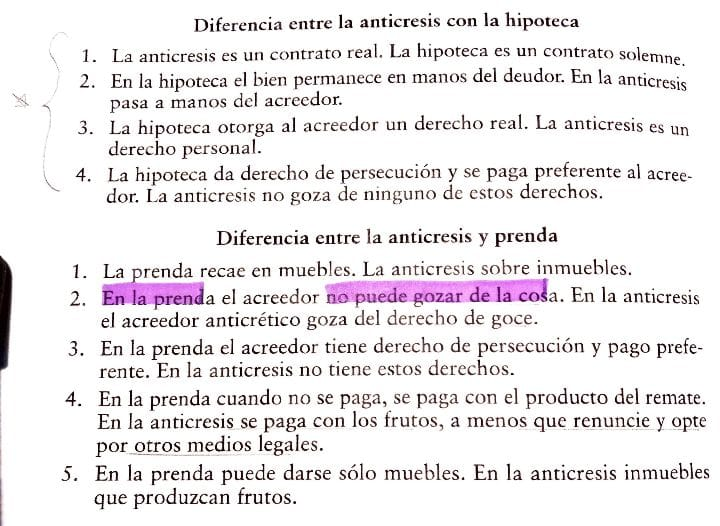
\includegraphics{da.jpeg}
    \caption{Diferencias Anticresis}
    \end{figure}
  \end{itemize}
\item
  El Contrato de Transacción

  Características:

  \begin{itemize}
  \tightlist
  \item
    ppal
  \item
    consensual
  \item
    bilateral
  \item
    intuito personae
  \item
    oneroso
  \item
    puede o no ser TTD
  \item
    debe existir un derecho dudoso y concesiones o sacrificios
    recíprocos
  \end{itemize}

  Efectos:

  \begin{itemize}
  \tightlist
  \item
    equivalente jurisdiccional
  \item
    sólo respecto de las partes
  \item
    sólo respecto a objetos específicos
  \item
    es obligatoria
  \item
    produce efecto de cosa juzgada
  \end{itemize}
\item
  El Juego y la Apuesta

  ppales contratos aleatorios:

  \begin{itemize}
  \tightlist
  \item
    ctto. de seguro
  \item
    préstamo a la gruesa ventura
  \item
    juego
  \item
    apuesta
  \item
    constitución de renta vitalicia
  \item
    constitución de censo vitalicio
  \end{itemize}
\item
  La Renta Vitalicia

  Características:

  \begin{itemize}
  \tightlist
  \item
    es un ctto real
  \item
    aleatorio
  \item
    ppal
  \item
    unilateral
  \item
    oneroso
  \end{itemize}
\item
  El censo

  Características

  \begin{itemize}
  \tightlist
  \item
    es un derecho real
  \item
    contrato ppal
  \item
    solemne
  \item
    capital siempre en dinero o estimarse en dinero
  \end{itemize}

  Constitución:

  \begin{itemize}
  \tightlist
  \item
    testamento
  \item
    donación
  \item
    venta
  \end{itemize}

  Causales de extinción:

  \begin{itemize}
  \tightlist
  \item
    abandono que el censuario hace de la cosa a favor del censualista
  \item
    redención del censo art. 2038
  \item
    destrucción completa de la finca
  \item
    prescripción
  \end{itemize}
\item
  El Contrato de Sociedad

  \begin{itemize}
  \tightlist
  \item
    Sociedad Colectiva
  \end{itemize}

  Es aquella en que todos los socios administran por sí o por un
  mandatario elegido de común acuerdo. Su administración puede confiarse
  a uno o más socios, sea por el contrato de sociedad o por un acto
  posterior.

  \begin{itemize}
  \tightlist
  \item
    Características:

    \begin{itemize}
    \tightlist
    \item
      consensual, salvo las sociedades comerciales y las civiles de
      responsabilidad limitada
    \item
      es intuito personae
    \item
      bilateral
    \item
      oneroso
    \item
      conmutativo 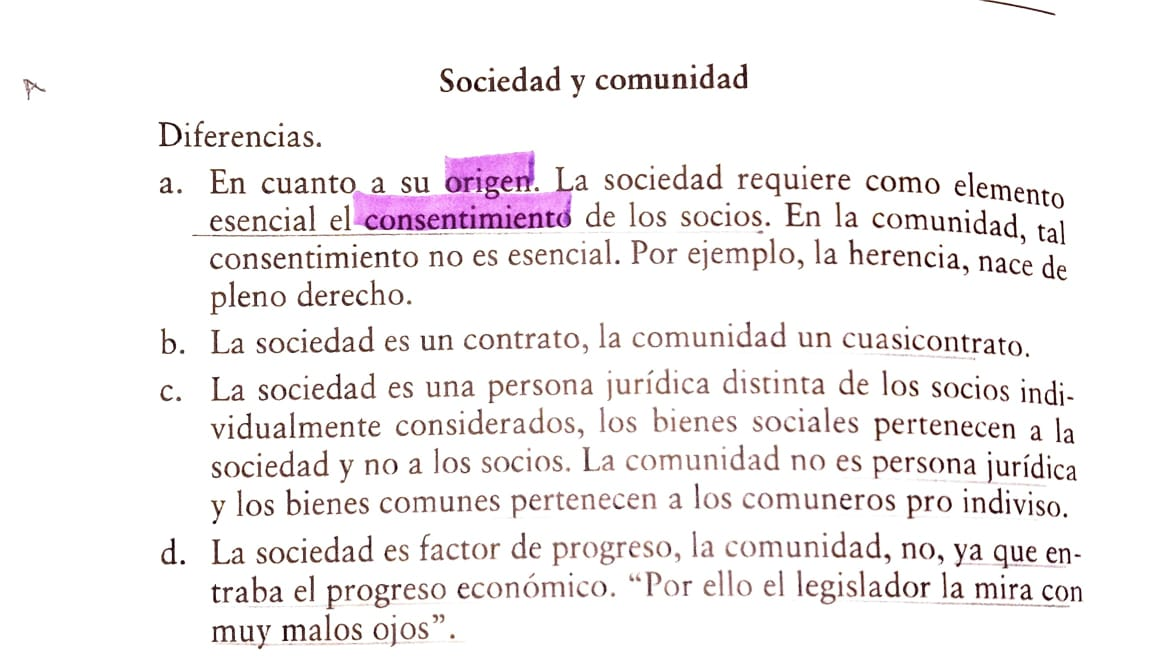
\includegraphics{dsc.jpeg}
    \end{itemize}
  \end{itemize}

  Elementos:

  \begin{itemize}
  \tightlist
  \item
    aporte
  \item
    participación en las utilidades
  \item
    contribución en las pérdidas
  \item
    intención de formar una sociedad
  \end{itemize}

  Disolución:

  \begin{itemize}
  \tightlist
  \item
    expiración del plazo o evento de una condición
  \item
    al finalizar el negocio para la cual fue contraída
  \item
    insolvencia
  \item
    pérdida de los bienes sociales
  \item
    incumplimiento de la obligación de realizar el aporte
  \item
    muerte de uno de los socios
  \end{itemize}
\item
  Contrato de Depósito

  Características:

  \begin{itemize}
  \tightlist
  \item
    contrato real
  \item
    unilateral
  \item
    por rg. es gratuito
  \item
    contrato ppal.
  \end{itemize}

  Obligaciones del depositario:

  \begin{itemize}
  \tightlist
  \item
    guardar y cuidar la cosa

    \begin{itemize}
    \tightlist
    \item
      responde de culpa grave
    \end{itemize}
  \item
    restituir la cosa a requerimiento del depositante
  \end{itemize}
\item
  El Comodato

  Características:

  \begin{itemize}
  \tightlist
  \item
    ctto unilateral
  \item
    gratuito
  \item
    real
  \item
    es un título de mera tenencia
  \item
    puede probarse por testigos
  \item
    es ppal
  \item
    comodatario responde de culpa levísima
  \end{itemize}

  Obligaciones del comodatario:

  \begin{itemize}
  \tightlist
  \item
    debe cuidar la cosa con la máxima diligencia, responde de culpa
    levísima
  \item
    usar la cosa según el uso autorizado en el ctto
  \item
    su infracción genera la obligación de indemnizar y autoriza para
    terminar el ctto de forma anticipada
  \item
    debe restituir en el plazo establecido o al terminar su uso
  \end{itemize}

  Obligaciones del comodante:

  \begin{itemize}
  \tightlist
  \item
    pagar las expensas y perjuicios
  \item
    indemnizar perjuicios por mala calidad o condición de lla cosa
    prestada
  \end{itemize}
\item
  Mutuo o Préstamo de Consumo

  Características:

  \begin{itemize}
  \item
    es un ctto real
  \item
    TTD
  \item
    unilateral
  \item
    no hay obligación de custodia
  \item
    naturalmente gratuito
  \item
    ctto ppal
  \item
    sólo sobre cosas fungibles

    \begin{figure}
    \centering
    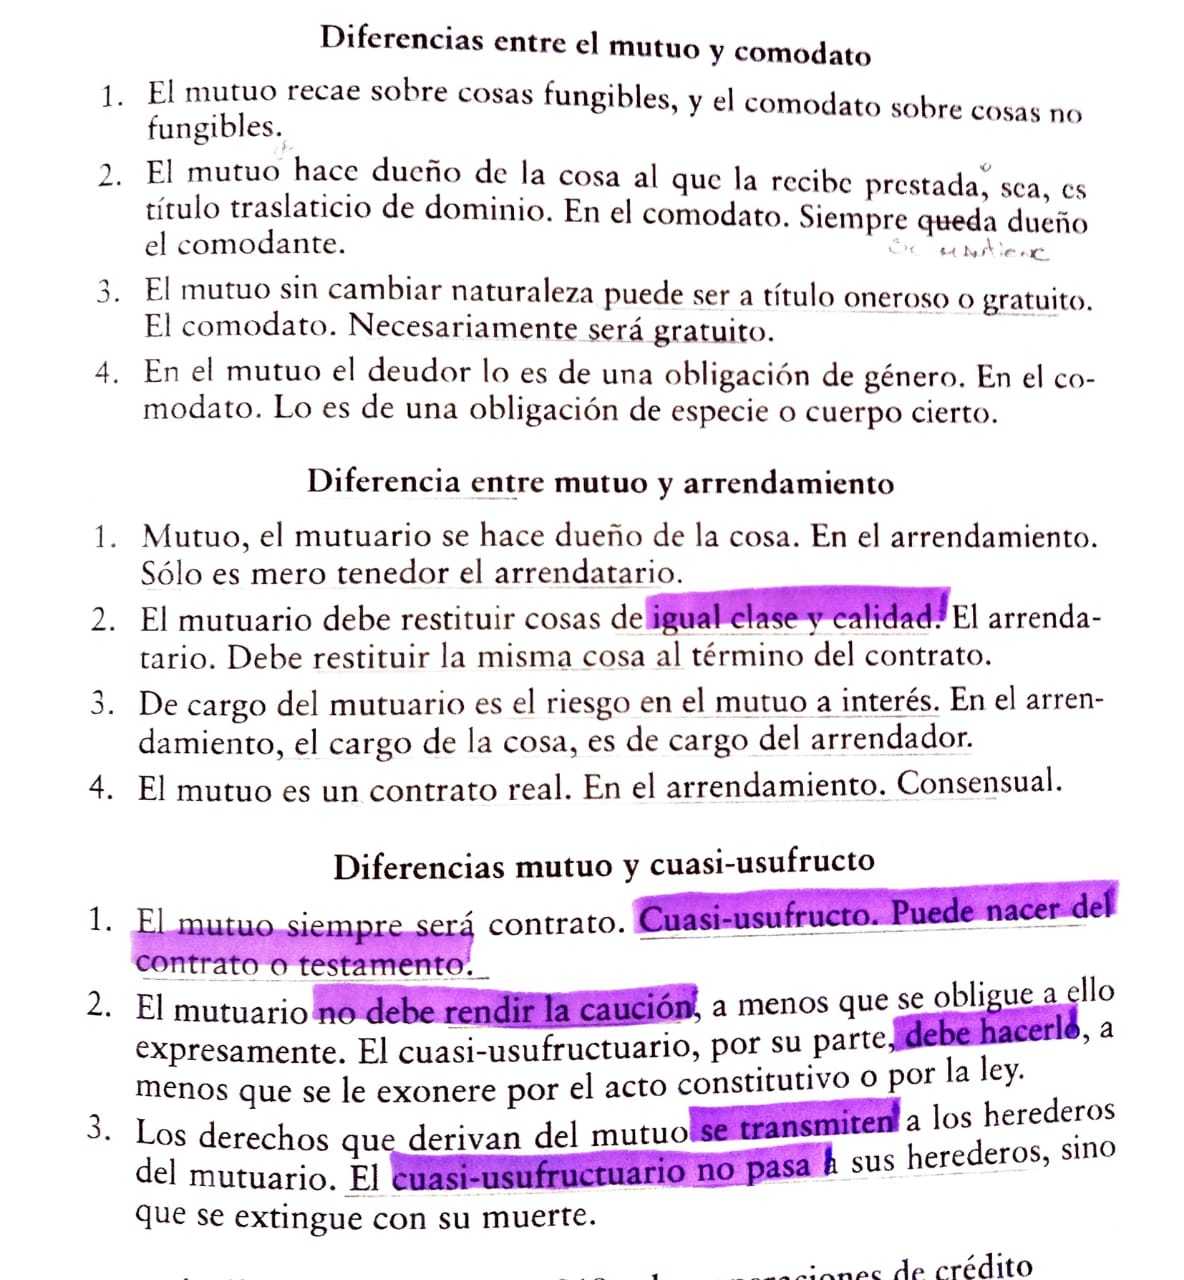
\includegraphics{difmutuo.jpeg}
    \caption{Diferencias Mutuo}
    \end{figure}
  \end{itemize}
\item
  Donación Revocable o entre vivos

  Pueden ser otorgados conforme a las normas de:

  \begin{itemize}
  \tightlist
  \item
    solemnidades del testamento
  \item
    solemnidades de las donaciones entre vivos
  \end{itemize}

  Tiene importancia respecto a su confirmación:

  \begin{itemize}
  \tightlist
  \item
    si es conforme al testamento quedará confirmada ipso iure con el
    fallecimiento
  \item
    si es conforme a la donación entre vivos (reservándose la facultad
    de revocarla), será necesario que el causante confirme en el
    testamento.
  \end{itemize}
\end{itemize}

\hypertarget{cuasicontratos}{%
\subsection{6.3. Cuasicontratos}\label{cuasicontratos}}

Esta institución reacciona frente al enriquecimiento injusto, otorgando
el derecho de indemnización

Principales cuasicontratos (art. 2285): - Agencia Oficiosa - no debe
existir mandato - debe actuar en interés del interesado - debe existir
de parte del gestor, la intención de crear un vínculo obligatorio en el
interesado - diferencias con el mandato: - mandato es un ctto - mandante
debe ser capaz, el interesado no requiere serlo - mandatario se obliga
independientemente del beneficio, el interesado se obliga con la
condición de que la gestión le sea útil y en su medida - El Pago de lo
No Debido - La Comunidad

\begin{verbatim}
Origen:
- en un hecho
- en un acto jurídico

Derechos de los comuneros:
- usar y gozar los bienes comunes
- derecho de oponerse a los actos de administración de otros
- derecho del comunero a enajenar su cuota

Obligaciones de los comuneros:
- contribuir a las expensas de conservación
- derecho a las innovaciones en los bienes comunes, con el consentimiento previo de los demás
- a hacer la partición cuando alguno lo pida
- los frutos se dividen a prorrata

Terminación de la comunidad:
- por la confusión de la cuota de todos los comuneros en una sola persona
- destrucción de la cosa común
- por la división del haber común
\end{verbatim}

\hypertarget{delitos-y-cuasidelito}{%
\subsection{6.4. Delitos y Cuasidelito}\label{delitos-y-cuasidelito}}

Las obligaciones también nacen de un hecho que ha inferido injuria o
daño a otra persona, como los delitos y cuasidelitos. Art. 1437.

Diferencias entre responsabilidad penal y civil - acción civil, acción
penal - sanción penal es represiva, la civil es indemnizadora - distinta
jurisdicción - capacidad penal 16-18, civil 7-16 - la penal es
personalísima, la civil se transmite - acción penal prescribe de 6 meses
a 15 años, la civil en 4 años

Diferencias entre responsabilidad contractual y extracontractual -
contractual existe un vínculo jurídico preexistente - culpa contractual
acepta graduaciones - capacidad contractual se adquiere a los 18 - en la
extracontractual se presume la solidaridad - contractual prescribe en 5
años y la extracontractual en 4 años

Elementos de la responsabilidad: - daño - dolo o culpa - hechos que
alteran o eximen la responsabilidad: - caso fortuito - estado de
necesidad - hecho de un tercero - culpa de la víctima - eximentes de la
responsabilidad - convenciones sobre responsabilidad extracontractual -
relación de causalidad - capacidad

\hypertarget{derechos-de-familia}{%
\section{7. Derechos de Familia}\label{derechos-de-familia}}

\begin{itemize}
\item
  El Matrimonio

  Requisitos:

  \begin{itemize}
  \tightlist
  \item
    de existencia

    \begin{itemize}
    \tightlist
    \item
      diversidad de sexo
    \item
      consentimiento
    \item
      presencia del oficial del RC
    \end{itemize}
  \item
    de validez

    \begin{itemize}
    \tightlist
    \item
      ambos sean legalmente capaces
    \item
      que hayan consentido libre y espontáneamente
    \end{itemize}
  \end{itemize}

  Impedimentos:

  \begin{itemize}
  \tightlist
  \item
    dirimentes - obstan al matrimonio (nulidad)

    \begin{itemize}
    \tightlist
    \item
      absolutos (respecto a cualquier personas)

      \begin{itemize}
      \tightlist
      \item
        hallarse ligado por vínculo matrimonial no disuelto
      \item
        menores de 16 años
      \item
        hallarse privado del uso de la razón, trastorno o anomalía
        psíquica, sea incapaz de modo absoluto de formar comunidad de
        vida que implica el matrimonio
      \item
        los que carecen de suficiente juicio o discernimiento para
        comprender y comprometerse en matrimonio
      \item
        los que no pudieren expresar claramente su voluntad por
        cualquier medio
      \end{itemize}
    \item
      relativos

      \begin{itemize}
      \tightlist
      \item
        por parentesco
      \item
        por homicidio
      \end{itemize}
    \end{itemize}
  \item
    impedientes (o prohibiciones)

    \begin{itemize}
    \tightlist
    \item
      por falta de asenso o licencia
    \item
      de guarda, entre pupilos y guardadores
    \item
      de segundas nupcias, respecto de los hijos de precedente
      matrimonio
    \end{itemize}
  \end{itemize}

  Formalidades:

  \begin{itemize}
  \item
    Matrimonios celebrados en Chile

    \begin{itemize}
    \item
      la manifestación o comunicación
    \item
      la información
    \item
      la celebración

      plazo de 90 días para celebrarse
    \item
      posteriores a la celebración:

      \begin{itemize}
      \tightlist
      \item
        acta de todo lo obrado, firmada por el oficial, los contrayentes
        y testigos
      \item
        se inscribirá los libros correspondientes
      \item
        omisión no acarrea nulidad
      \end{itemize}
    \end{itemize}
  \item
    Matrimonio celebrado en el extranjero

    art. 80 LMC, los requisitos de forma y de fondo del matrimonio serán
    los que establezca la ley \textbf{del lugar} de su celebración.
  \item
    Matrimonios celebrados ante entidades religiosas de derecho público

    Producirán los mismos efectos que el matrimonio civil, siempre que
    cumplan con los requisitos contemplados en la ley, desde su
    inscripción

    Formalidades:

    \begin{itemize}
    \tightlist
    \item
      otorgamiento de acta
    \item
      plazo de 8 días para su inscripción
    \end{itemize}
  \item
    Efectos del matrimonio

    \begin{itemize}
    \tightlist
    \item
      crea un conjunto de derechos y obligaciones
    \item
      genera una sociedad universal que comprende los patrimonios de los
      cónyuges
    \item
      da origen a la filiación matrimonial
    \item
      crea entre los cónyuges la obligación de prestarse pensiones
      alimenticias
    \item
      transforma a los cónyuges en herederos recíprocos
    \item
      derecho a solicitar la declaración de bienes familiares
    \end{itemize}
  \item
    Terminación del matrimonio

    \begin{itemize}
    \tightlist
    \item
      muerte natural de un cónyuge
    \item
      muerte presunta
    \item
      sentencia firme que declara la nulidad del matrimonio
    \item
      sentencia firme de divorcio
    \item
      sentencia firme que acoge la rectificación de sexo y nombre por
      razón de identidad de género
    \end{itemize}
  \end{itemize}
\item
  Separación

  \begin{itemize}
  \item
    Separación de Hecho

    Mera separación de cuerpos, cuyo objeto es regular especialmente la
    materia de alimentos, régimen de bienes y en su caso el cuidado
    personal y la relación directa y regular

    \begin{itemize}
    \tightlist
    \item
      si no hubo prole:

      \begin{itemize}
      \tightlist
      \item
        regular sus relaciones mutuas
      \item
        los alimentos
      \item
        régimen de bienes del matrimonio
      \end{itemize}
    \item
      si hubo:

      \begin{itemize}
      \tightlist
      \item
        regular además el régimen aplicable a los alimentos
      \item
        cuidado personal y a la relación directa y regular que mantendrá
        con los hijos aquél que no tuviere bajo su cuidado
      \end{itemize}
    \item
      Formas de regular:

      \begin{itemize}
      \item
        de común acuerdo

        \begin{itemize}
        \item
          Formalidades (para dar fecha cierta al cese de convivencia)

          \begin{itemize}
          \tightlist
          \item
            Escritura pública
          \item
            acta extendida y protocolizada ante notario
          \item
            acta extendida ante oficial del RC
          \item
            transacción aprobada judicialmente
          \item
            notificación de la demanda, caso del art. 23
            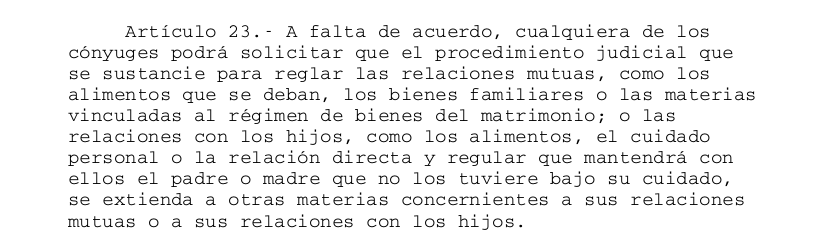
\includegraphics{23lmc.png}
          \end{itemize}
        \end{itemize}
      \item
        regulación judicial

        En forma subsidiaria
      \end{itemize}
    \end{itemize}
  \item
    Separación Judicial

    \begin{itemize}
    \item
      por uno de los cónyuges si hay falta imputable al otro

      Es una acción irrenunciable
    \item
      por cualquiera si hay cese de convivencia
    \item
      de forma conjunta, acompañando acuerdo completo y suficiente
    \end{itemize}

    Efectos de la separación judicial:

    \begin{itemize}
    \tightlist
    \item
      desde que se dicta la sentencia y quede ejecutoriada
    \item
      no pueden casarse
    \item
      subsisten todos los derechos y obligaciones personales
    \item
      terminan los regímenes matrimoniales
    \item
      no se alteran los derechos hereditarios
    \item
      no alteran la filiación
    \item
      no goza de presunción de paternidad
    \end{itemize}
  \end{itemize}
\item
  Nulidad del Matrimonio

  Causales:

  \begin{itemize}
  \item
    por alguna de las incapacidades señaladas en los art. 5,6,7

    \begin{itemize}
    \tightlist
    \item
      ligados por vínculo matrimonial no disuelto
    \item
      menores de 16
    \item
      privados de razón
    \item
      carecer de suficiente juicio o discernimiento
    \item
      no poder expresar claramente su voluntad
    \item
      por parentesco (ascendientes y descendientes, por consanguinidad o
      afinidad, ni los colaterales por consanguinidad en 2do grado)
    \item
      el caso del homicidio del cónyuge(formalizado o condenado)
    \end{itemize}
  \item
    consentimiento no hubiere sido libre y espontáneo
  \item
    no celebrado ante el número de testigos hábiles
  \item
    Titularidad

    Corresponde a cualquiera de los cónyuges, salvo:

    \begin{itemize}
    \tightlist
    \item
      menores de 16 = solamente los que contrajeron sin tener la edad
      exigida = dentro de 1 año, empieza a correr una vez cumplida la
      mayoría de edad
    \item
      error o fuerza = solamente el que las han sufrido = 3 años, desde
      que hubiere desaparecido el hecho que origina el vicio
    \item
      matrimonio celebrado en art. de muerte = también corresponde a los
      herederos del difunto = 1 año desde el fallecimiento
    \item
      vínculo matrimonial no disuelto = también al cónyuge anterior o
      sus herederos = 1 año al fallecimiento de uno de los cónyuges
    \item
      por parentesco u homicidio = también por cualquier persona con
      interés en la moral o de la ley = 1 año desde la celebración del
      matrimonio
    \end{itemize}
  \end{itemize}

  Efectos de la declaración de nulidad

  \begin{itemize}
  \tightlist
  \item
    retroactivamente
  \item
    debe subinscribirse al margen de la respectiva inscripción
    matrimonial
  \item
    si uno de los cónyuges hubiese contraído matrimonio nuevamente, es
    válido
  \item
    las capitulaciones matrimoniales caducan
  \item
    no ha habido sociedad conyugal ni participación en los gananciales
  \item
    no ha habido parentesco por afinidad
  \item
    los hijos son matrimoniales
  \item
    se presume que los cónyuges han contraído matrimonio de buena fe y
    justa causa de error
  \end{itemize}
\item
  El Divorcio

  \begin{itemize}
  \tightlist
  \item
    unilateral

    \begin{itemize}
    \tightlist
    \item
      atentado contra la vida o malos tratamientos graves contra la
      integridad física o psíquica del cónyuge o de algunos de los hijos
    \item
      trasgresión grave y reiterada de los deberes de convivencia,
      socorro y fidelidad propios del matrimonio
    \item
      condena ejecutoriada por la comisión de crímenes o simples delitos
      contra el orden de las familias y contra la moralidad pública
    \item
      conducta homosexual
    \item
      alcoholismo o drogadicción
    \item
      tentativa de prostituir al otro o sus hijos
    \end{itemize}
  \item
    de común acuerdo

    \begin{itemize}
    \tightlist
    \item
      cese de convivencia mayor de 1 año
    \item
      debe acompañarse acuerdo completo y suficiente
    \end{itemize}
  \item
    por trascurso del tiempo

    \begin{itemize}
    \tightlist
    \item
      3 años de cese de convivencia
    \end{itemize}
  \item
    Efectos:

    \begin{itemize}
    \tightlist
    \item
      desde que la sentencia quede ejecutoriada
    \item
      deberá subinscribirse
    \item
      crea el estado civil de divorciado
    \item
      pone fin a las obligaciones y derechos de carácter patrimonial que
      se fundan en el matrimonio
    \end{itemize}
  \item
    Reglas comunes a la separación, nulidad y divorcio

    \begin{itemize}
    \tightlist
    \item
      Compensación económica
    \item
      Conciliación
    \end{itemize}
  \end{itemize}
\end{itemize}

\hypertarget{derecho-sucesorio}{%
\section{8. Derecho Sucesorio}\label{derecho-sucesorio}}

\end{document}
